\documentclass[aspectratio=169,10pt]{beamer}
% Beamer layout
\setbeamersize{text margin left=0.4cm, text margin right=0.2cm}

% Math & fonts
\usepackage{amsmath,amssymb}
\usepackage{mathpazo}   % Palatino text + math

% Tables & units
\usepackage{booktabs}
\usepackage{siunitx}

% TikZ (one load, all libs)
\usepackage{tikz}
\usetikzlibrary{arrows.meta,calc,positioning,shapes.geometric,shapes.misc}

% Algorithms
\usepackage{algorithm}
\usepackage[noend]{algpseudocode}
\usepackage{float}

% Media
\usepackage{multimedia}
\usepackage{animate}

% Bibliography
\usepackage{natbib}


\newcommand{\shortdate}{\the\month-\the\day}
\graphicspath{{../../figures/.}}


\definecolor{cardinalred}{RGB}{140,21,21}
\definecolor{coolgray}{RGB}{77,79,83}
\definecolor{black}{RGB}{0,0,0}
\definecolor{beige}{RGB}{210,194,149}
\definecolor{darkbeige}{RGB}{179,153,93}
\definecolor{darkcardinal}{RGB}{94,48,50}
\definecolor{lightcardinal}{RGB}{141,60,30}
\definecolor{darkpurple}{RGB}{83,40,79}
\definecolor{darkcyan}{RGB}{0,124,146}
\definecolor{skyblue}{RGB}{0,152,219}
\definecolor{treegreen}{RGB}{0,155,118}
\definecolor{darkorange}{RGB}{168,101,12}
\definecolor{beigegray}{RGB}{95,87,79}
\definecolor{boxgray}{RGB}{238,235,233}
\definecolor{footergray}{RGB}{199,209,197}



\mode<presentation>

\setbeamercolor*{palette primary}{use=structure,fg=white,bg= cardinalred}
\setbeamercolor*{palette secondary}{use=structure,fg=white,bg= coolgray}
\setbeamercolor*{palette tertiary}{use=structure,fg=white,bg= darkcardinal}
\setbeamercolor*{palette quaternary}{fg=white,bg= darkbeige}

\setbeamercolor*{sidebar}{use=structure,bg= beige}
\setbeamercolor*{footer}{use=structure,bg= footergray,fg=darkcardinal}
  
\setbeamercolor*{palette sidebar primary}{use=structure,fg=structure.fg!10}
\setbeamercolor*{palette sidebar secondary}{fg=white}
\setbeamercolor*{palette sidebar tertiary}{use=structure,fg=structure.fg!50}
\setbeamercolor*{palette sidebar quaternary}{fg=white}

\setbeamercolor*{titlelike}{parent=palette primary}
\setbeamercolor*{foot line}{parent=palette secondary}

\setbeamercolor*{separation line}{}
\setbeamercolor*{fine separation line}{}

\setbeamercolor{itemize item}{fg=cardinalred}
\setbeamercolor{itemize subitem}{fg=cardinalred}
\setbeamercolor{itemize subsubitem}{fg=cardinalred}
\setbeamercolor{enumerate item}{fg=cardinalred}
\setbeamercolor{enumerate subitem}{fg=cardinalred}
\setbeamercolor{enumerate subsubitem}{fg=cardinalred}
\setbeamercolor{description item}{fg=cardinalred}

\setbeamertemplate{bibliography item}[text]
\setbeamertemplate{frametitle continuation}[from second]
\setbeamercolor{bibliography entry title}{fg=black}
\setbeamercolor{bibliography entry author}{fg=black}
\setbeamercolor*{bibliography entry location}{fg=black}
\setbeamercolor*{bibliography entry note}{fg=black}

\renewcommand*{\bibfont}{\small}
\setbeamertemplate{navigation symbols}{}

\setbeamerfont{footnote}{size=\tiny}

\mode
<all>
\definecolor{cardinalred}{RGB}{140,21,21}
%--- Custom footline
\setbeamertemplate{footline}{%
\begin{beamercolorbox}[wd=\paperwidth,ht=4ex,dp=2.5ex]{}
    \centering
    \makebox[0.32\paperwidth][l]{\scriptsize\texttt{Pipe. \shortdate}}
    \makebox[0.32\paperwidth][c]{\scriptsize\texttt{$^{\dag}$masseyj@stanford.edu}}
    \makebox[0.32\paperwidth][r]{\scriptsize\insertframenumber/\inserttotalframenumber}
  \end{beamercolorbox}
}
\usepackage{algorithm}
\usepackage[noend]{algpseudocode}
\usetikzlibrary{arrows.meta,shapes.geometric,shapes.misc,positioning}

\tikzset{
  >={Stealth},
  proc/.style = {rectangle, rounded corners, draw, align=left, minimum height=8mm, text width=35mm, align=center},
  meas/.style    = {trapezium, trapezium left angle=70, trapezium right angle=110, draw, align=left, minimum height=8mm, text width=19mm, align=center},
  decision/.style = {diamond, aspect=2.2, draw, align=center, inner xsep=1.2ex, inner ysep=1ex, text width=2cm},
  smldec/.style = {diamond, aspect=2.2, draw, align=center, inner xsep=1.2ex, inner ysep=1ex, text width=19mm},
  terminator/.style = {ellipse, draw, align=center, minimum height=8mm, minimum width=16mm},
  line/.style  = {->, line width=0.6pt}
}


%--- Title info
\title{Pressure signal processing}
\author{JMO Massey$^{\dag}$, F Cabrera-Booman, T Jaroslawski, JC Klewicki, BJ McKeon}
\institute{Center for Turbulence Research \\ Stanford University}
% \thanks{This work was supported by DARPA under the CHAOS program}
\date{\today}

\begin{document}

%--- Title page
\begin{frame}
    \setcounter{framenumber}{0}
    \titlepage
    \vfill
    {\scriptsize \centering Thanks to DARPA for funding this work.\par}
\end{frame}

\begin{frame}
  \frametitle{Going from raw data to clean spectra}
  \begin{columns}[c] % vertically centered
    \column{0.42\textwidth}
    %   \includegraphics[width=\linewidth]{leftfig}
        Raw measurements from pinhole (PH) mic.
    
    \column{0.10\textwidth}
      \centering
      \scalebox{3}{$\Longrightarrow$}
    \column{0.42\textwidth}
    %   \includegraphics[width=\linewidth]{rightfig}
        Cleaned pressure spectra.
    
  \end{columns}
\end{frame}

\begin{frame}
    \begin{figure}
    \centering
    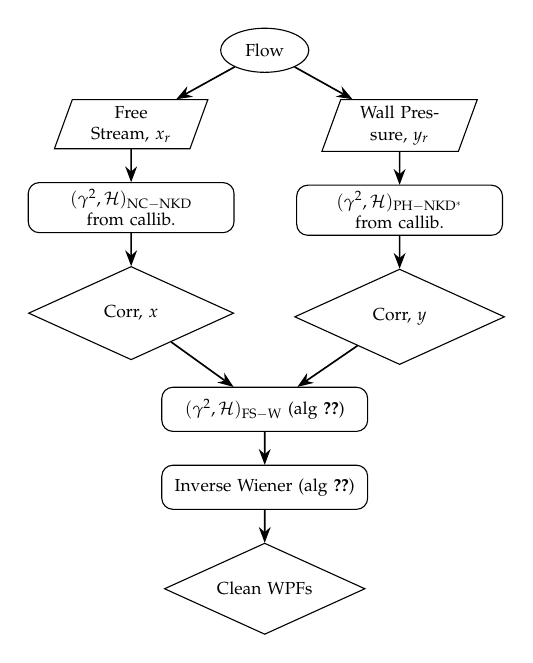
\begin{tikzpicture}[scale=0.7, transform shape, node distance=6mm and 18mm,
                    every node/.style={font=\small}]
        \centering
    % Start
        \node (start) [terminator] {Flow};

        % Two separate measurement boxes
        \node (refraw)   [meas, below left = 6mm and 14mm of start, anchor=north east]
            {Free Stream, $x_r$};
            
        \node (tretraw) [meas, below right = 6mm and 14mm of start, anchor=north west]
            {Wall Pressure, $y_r$};

        \node (Href) [proc, below=of refraw]
            {$ (\gamma^2,\mathcal{H})_{\mathrm{NC-NKD}} $ from callib.};

        \node (ref) [decision, below=of Href]
            {Corr, $x$};


        \node (Htret)  [proc, below=of tretraw]
            {$ (\gamma^2,\mathcal{H})_{\mathrm{PH-NKD^*}} $ from callib.};

        \node (tret)  [decision, below=of Htret]
            {Corr, $y$};

        \node (Hcomb)  [proc, below=57mm of start]
            {$ (\gamma^2,\mathcal{H})_{\mathrm{FS-W}} $ (alg~\ref{alg:H})};

        \node (corr)  [proc, below=of Hcomb]
            {Inverse Wiener (alg~\ref{alg:inv})};

        \node (post)  [decision, below=of corr]
            {Clean WPFs};

        \draw [line] (start) -- (refraw);
        \draw [line] (refraw) -- (Href);
        \draw [line] (Href) -- (ref);
        \draw [line] (start) -- (tretraw);
        \draw [line] (tretraw) -- (Htret);
        \draw [line] (Htret) -- (tret);
        \draw [line] (tret) -- (Hcomb);
        \draw [line] (ref) -- (Hcomb);
        \draw [line] (Hcomb) -- (corr);
        \draw [line] (corr) -- (post);

    \end{tikzpicture}
    \caption{Complete pressure processing pipeline for measurement of the WPFs through a pinhole microphone.}
    \end{figure}
\end{frame}

\begin{frame}
    \frametitle{Microphone calibration: Naked (NKD)}
    \begin{columns}[c] % vertically centered
        \column{0.55\textwidth}
            \centering
            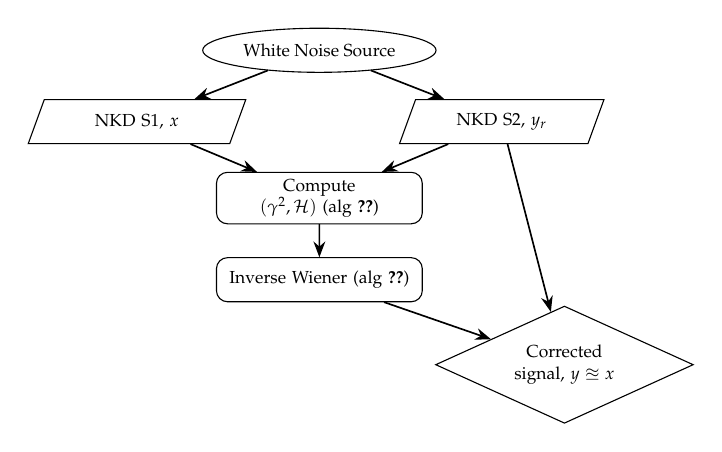
\begin{tikzpicture}[scale=0.7, transform shape,
                node distance=6mm and 18mm, every node/.style={font=\small}]
                \node (start) [terminator] {White Noise Source};

                % Two separate measurement boxes
                \node (ref)   [meas, below left = 6mm and 14mm of start, anchor=north east]
                    {NKD S1, $x$};
                \node (treat) [meas, below right = 6mm and 14mm of start, anchor=north west]
                    {NKD S2, $y_r$};

                \node (H)  [proc, below=18mm of start]
                    {Compute $(\gamma^2,\mathcal{H})$ (alg~\ref{alg:H})};

                \node (wien)  [proc, below=of H]
                    {Inverse Wiener (alg~\ref{alg:inv})};

                \node (corr)  [decision, below right = 6mm and 14mm of wien]
                    {Corrected signal, $y \approxeq x$};

                \draw [line] (start) -- (ref);
                \draw [line] (start) -- (treat);
                \draw [line] (ref) -- (H);
                \draw [line] (treat) -- (H);
                \draw [line] (H) -- (wien);
                \draw [line] (wien) -- (corr);
                \draw [line] (treat) -- (corr);

            \end{tikzpicture}
        \column{0.4\textwidth}
            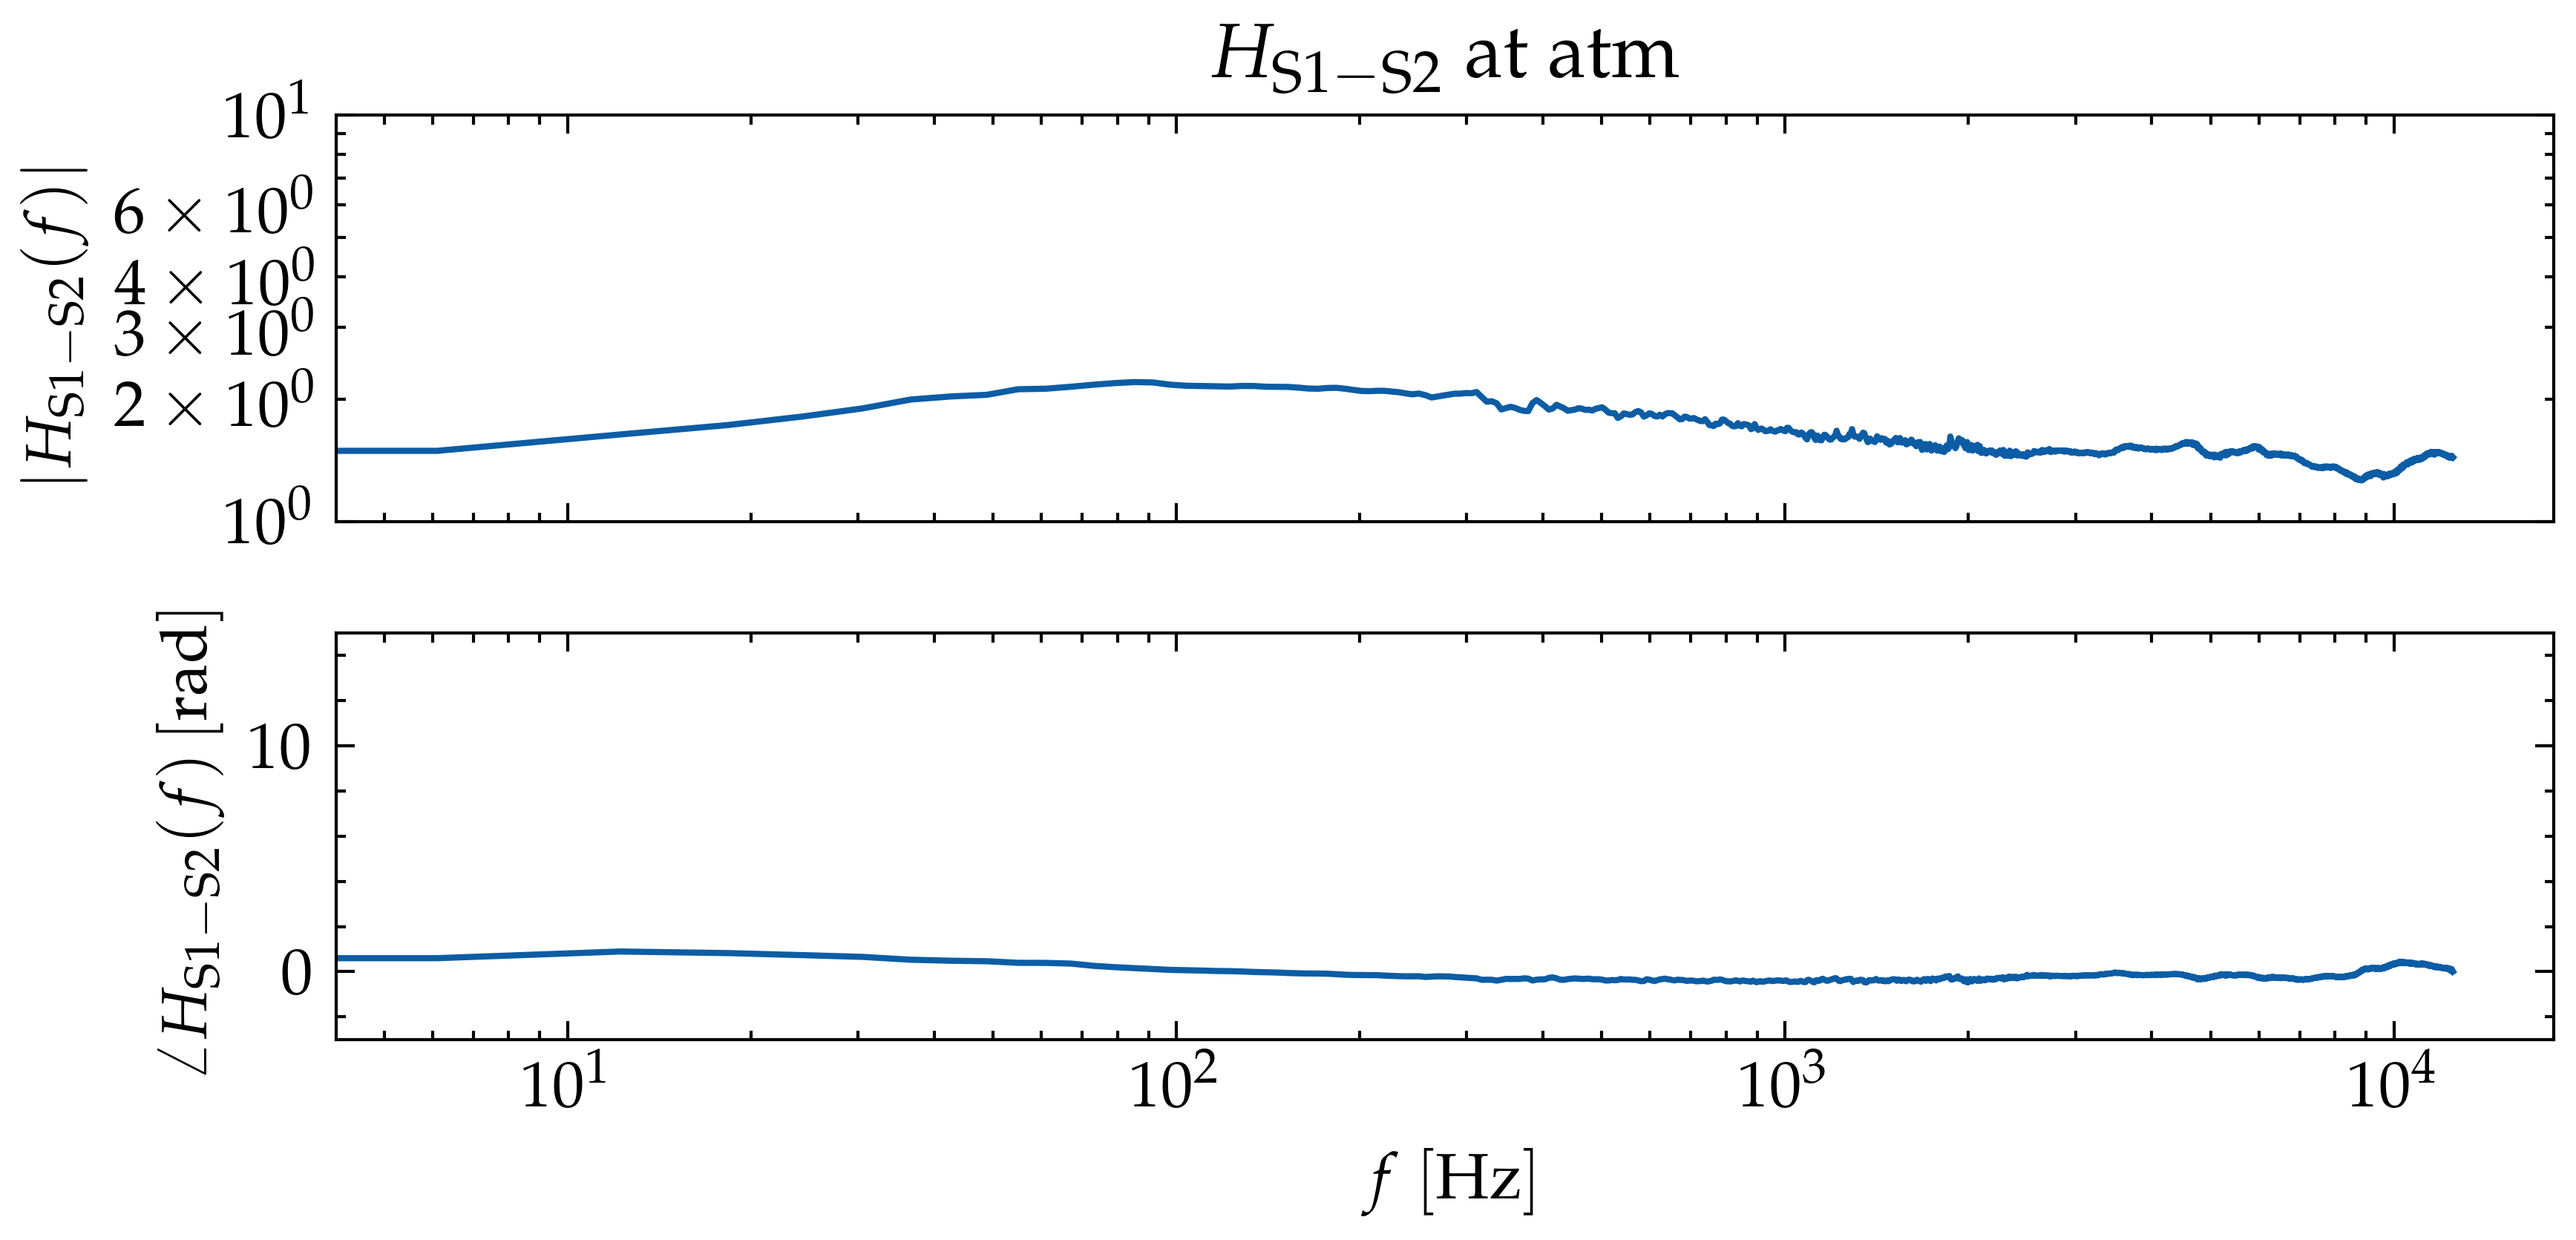
\includegraphics[width=0.8\linewidth]{S1-S2/H_atm.png}
            % 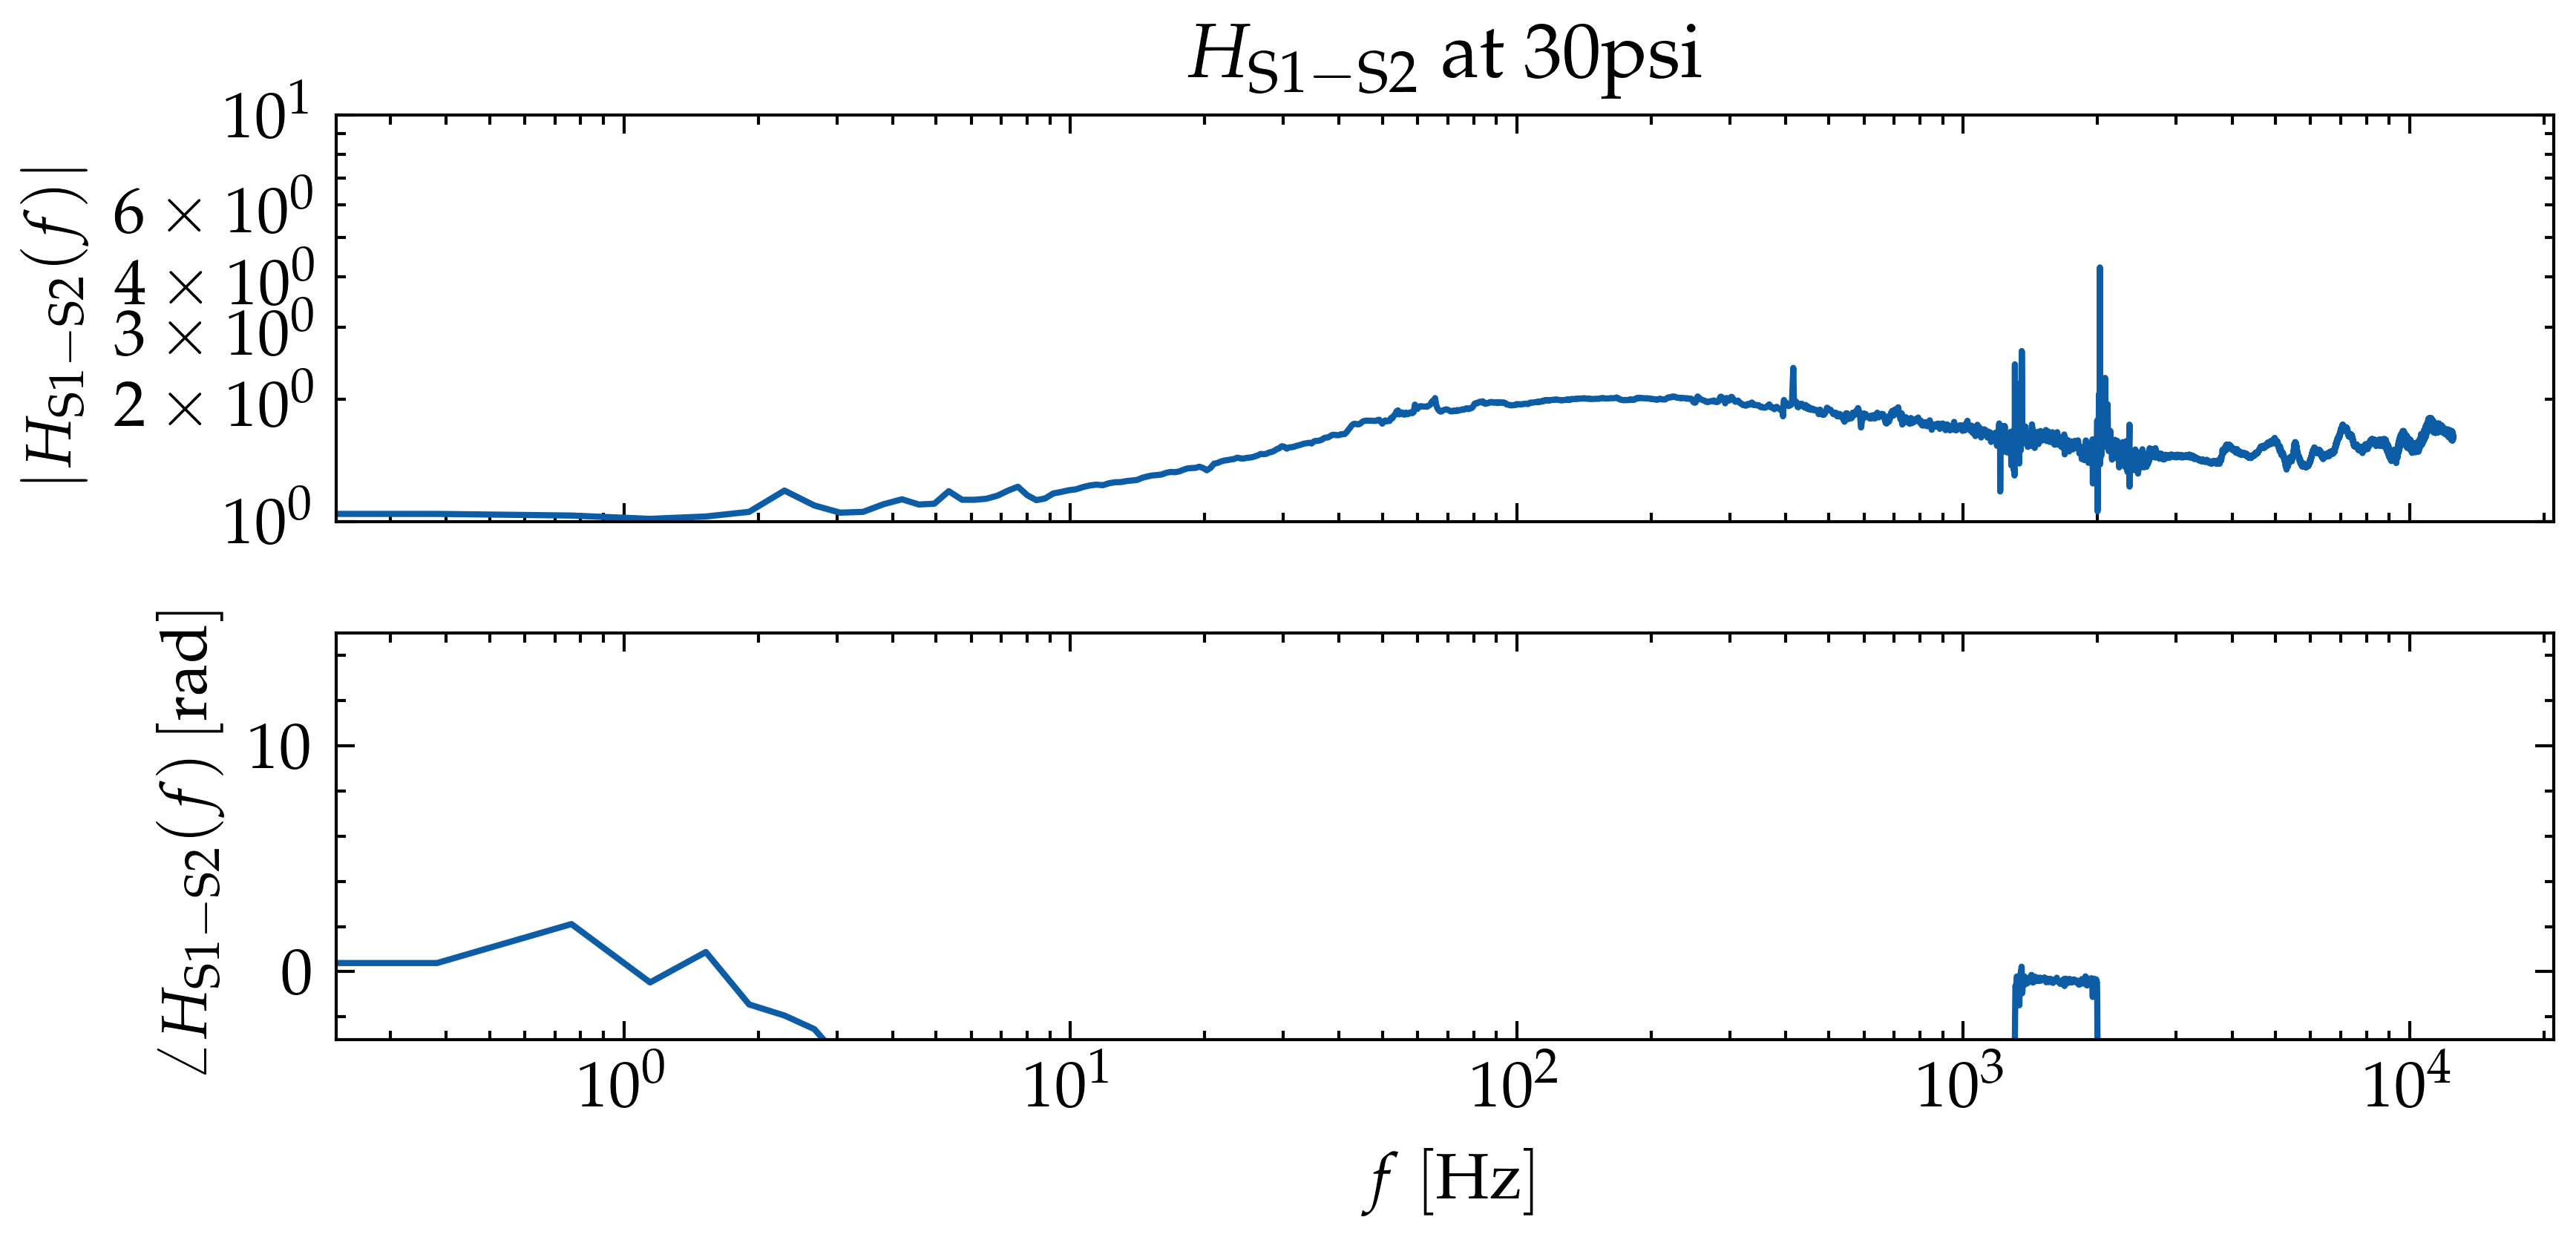
\includegraphics[width=0.8\linewidth]{S1-S2/H_30psi.png}
            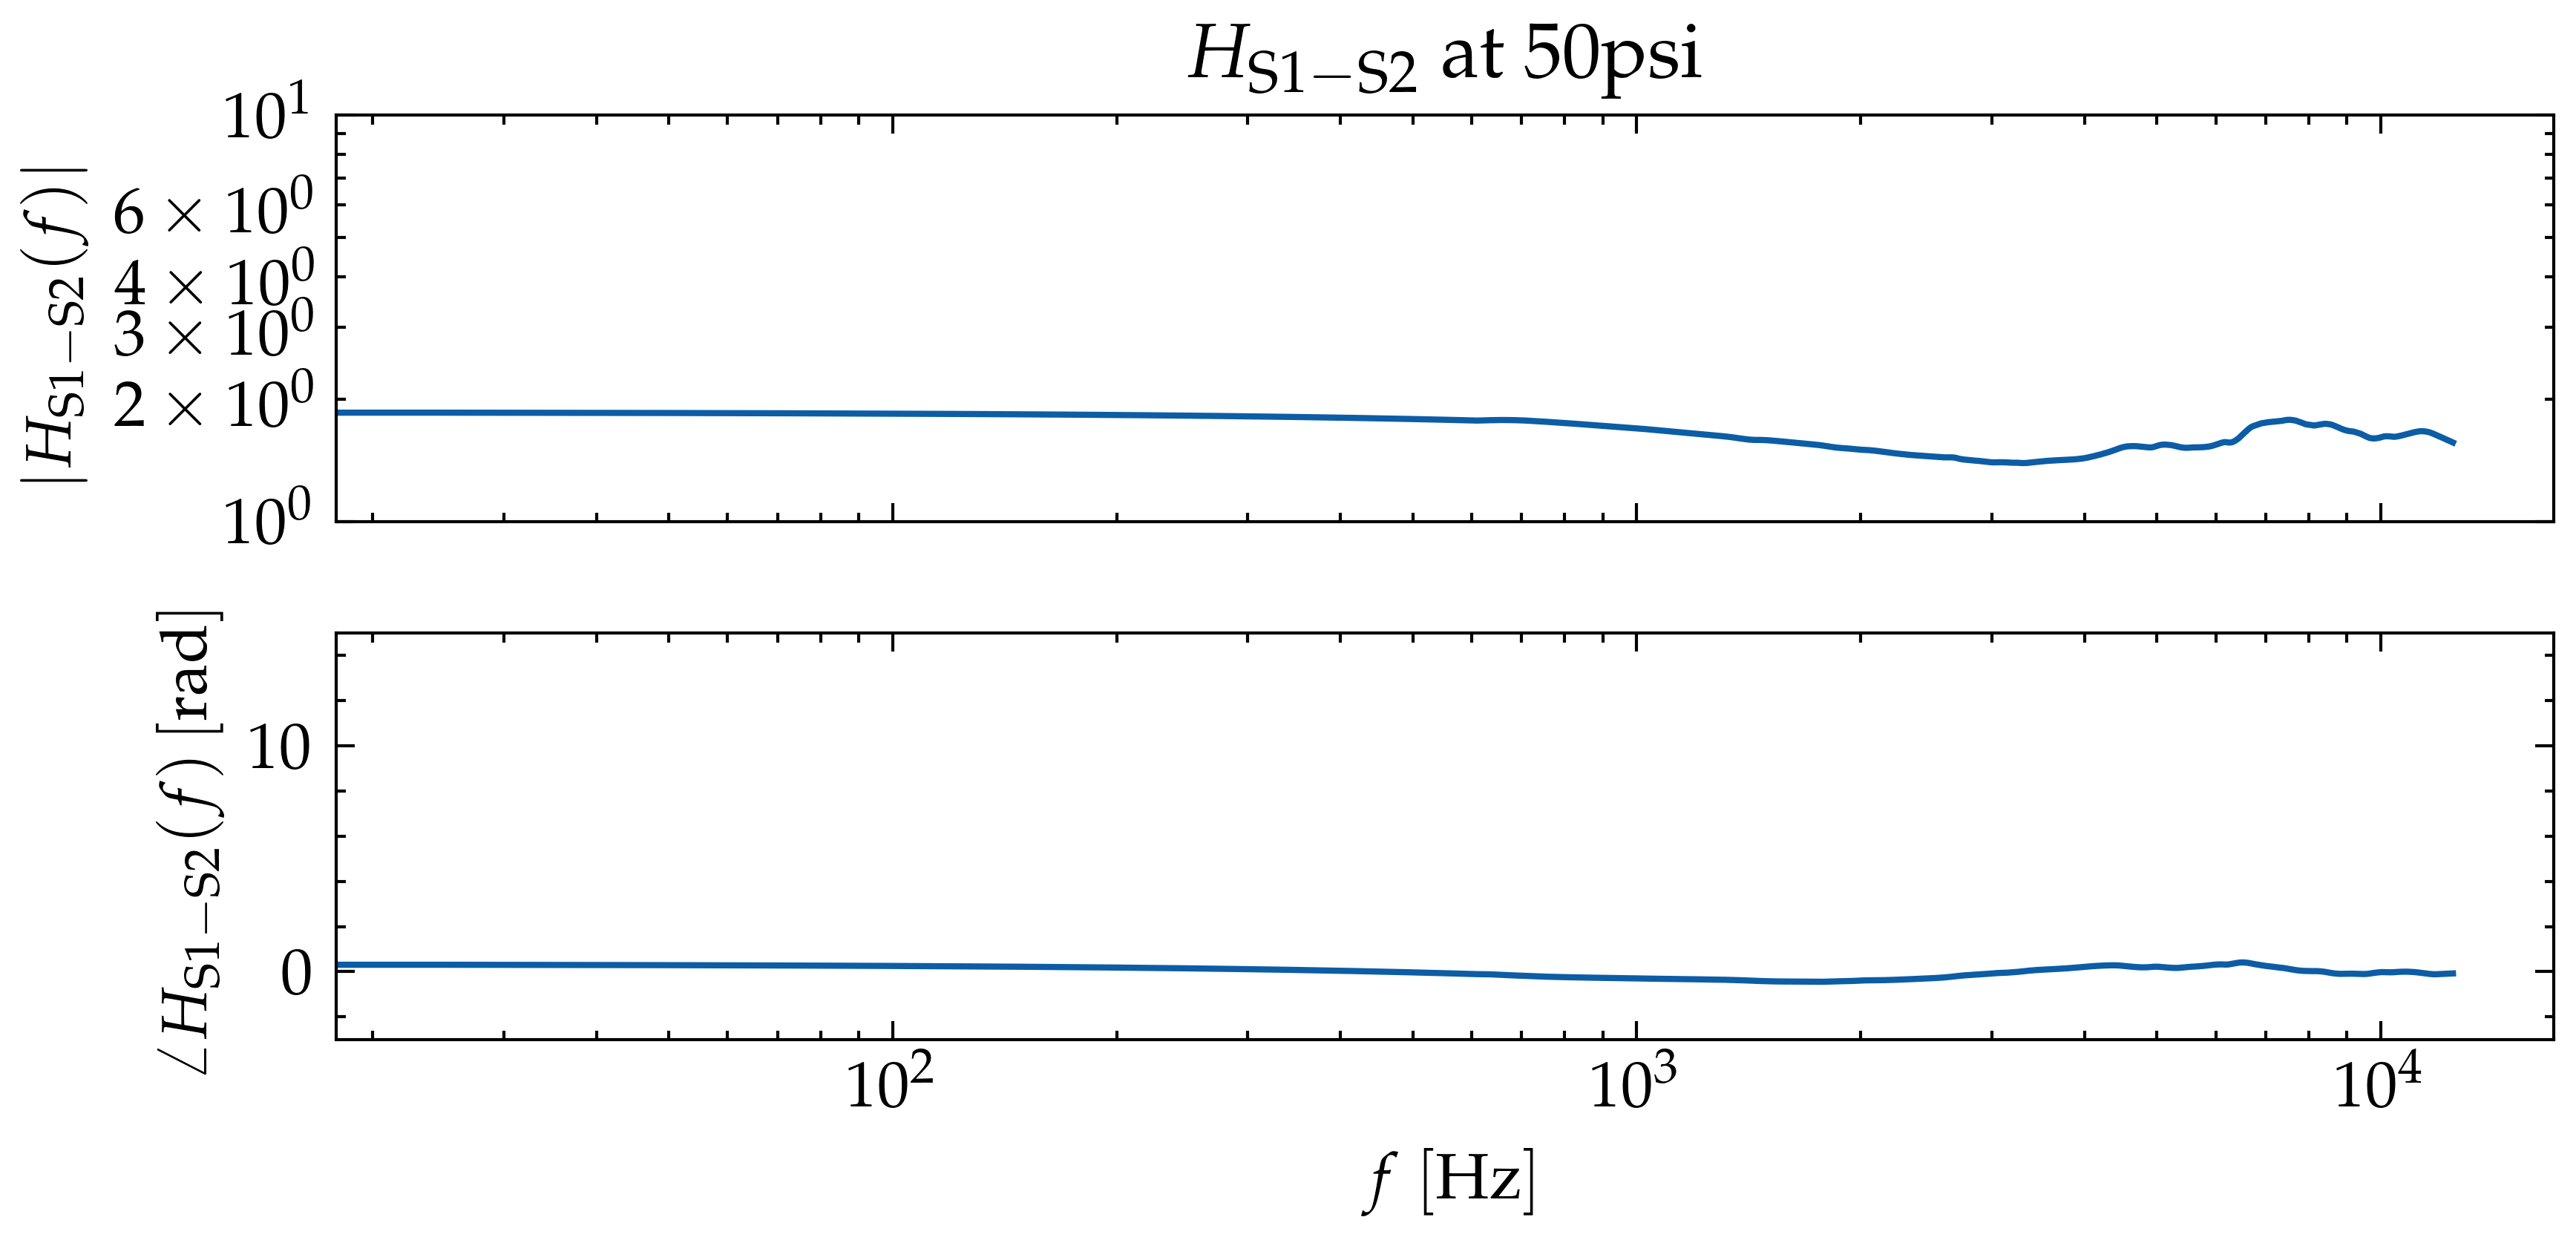
\includegraphics[width=0.8\linewidth]{S1-S2/H_50psi.png}
            % 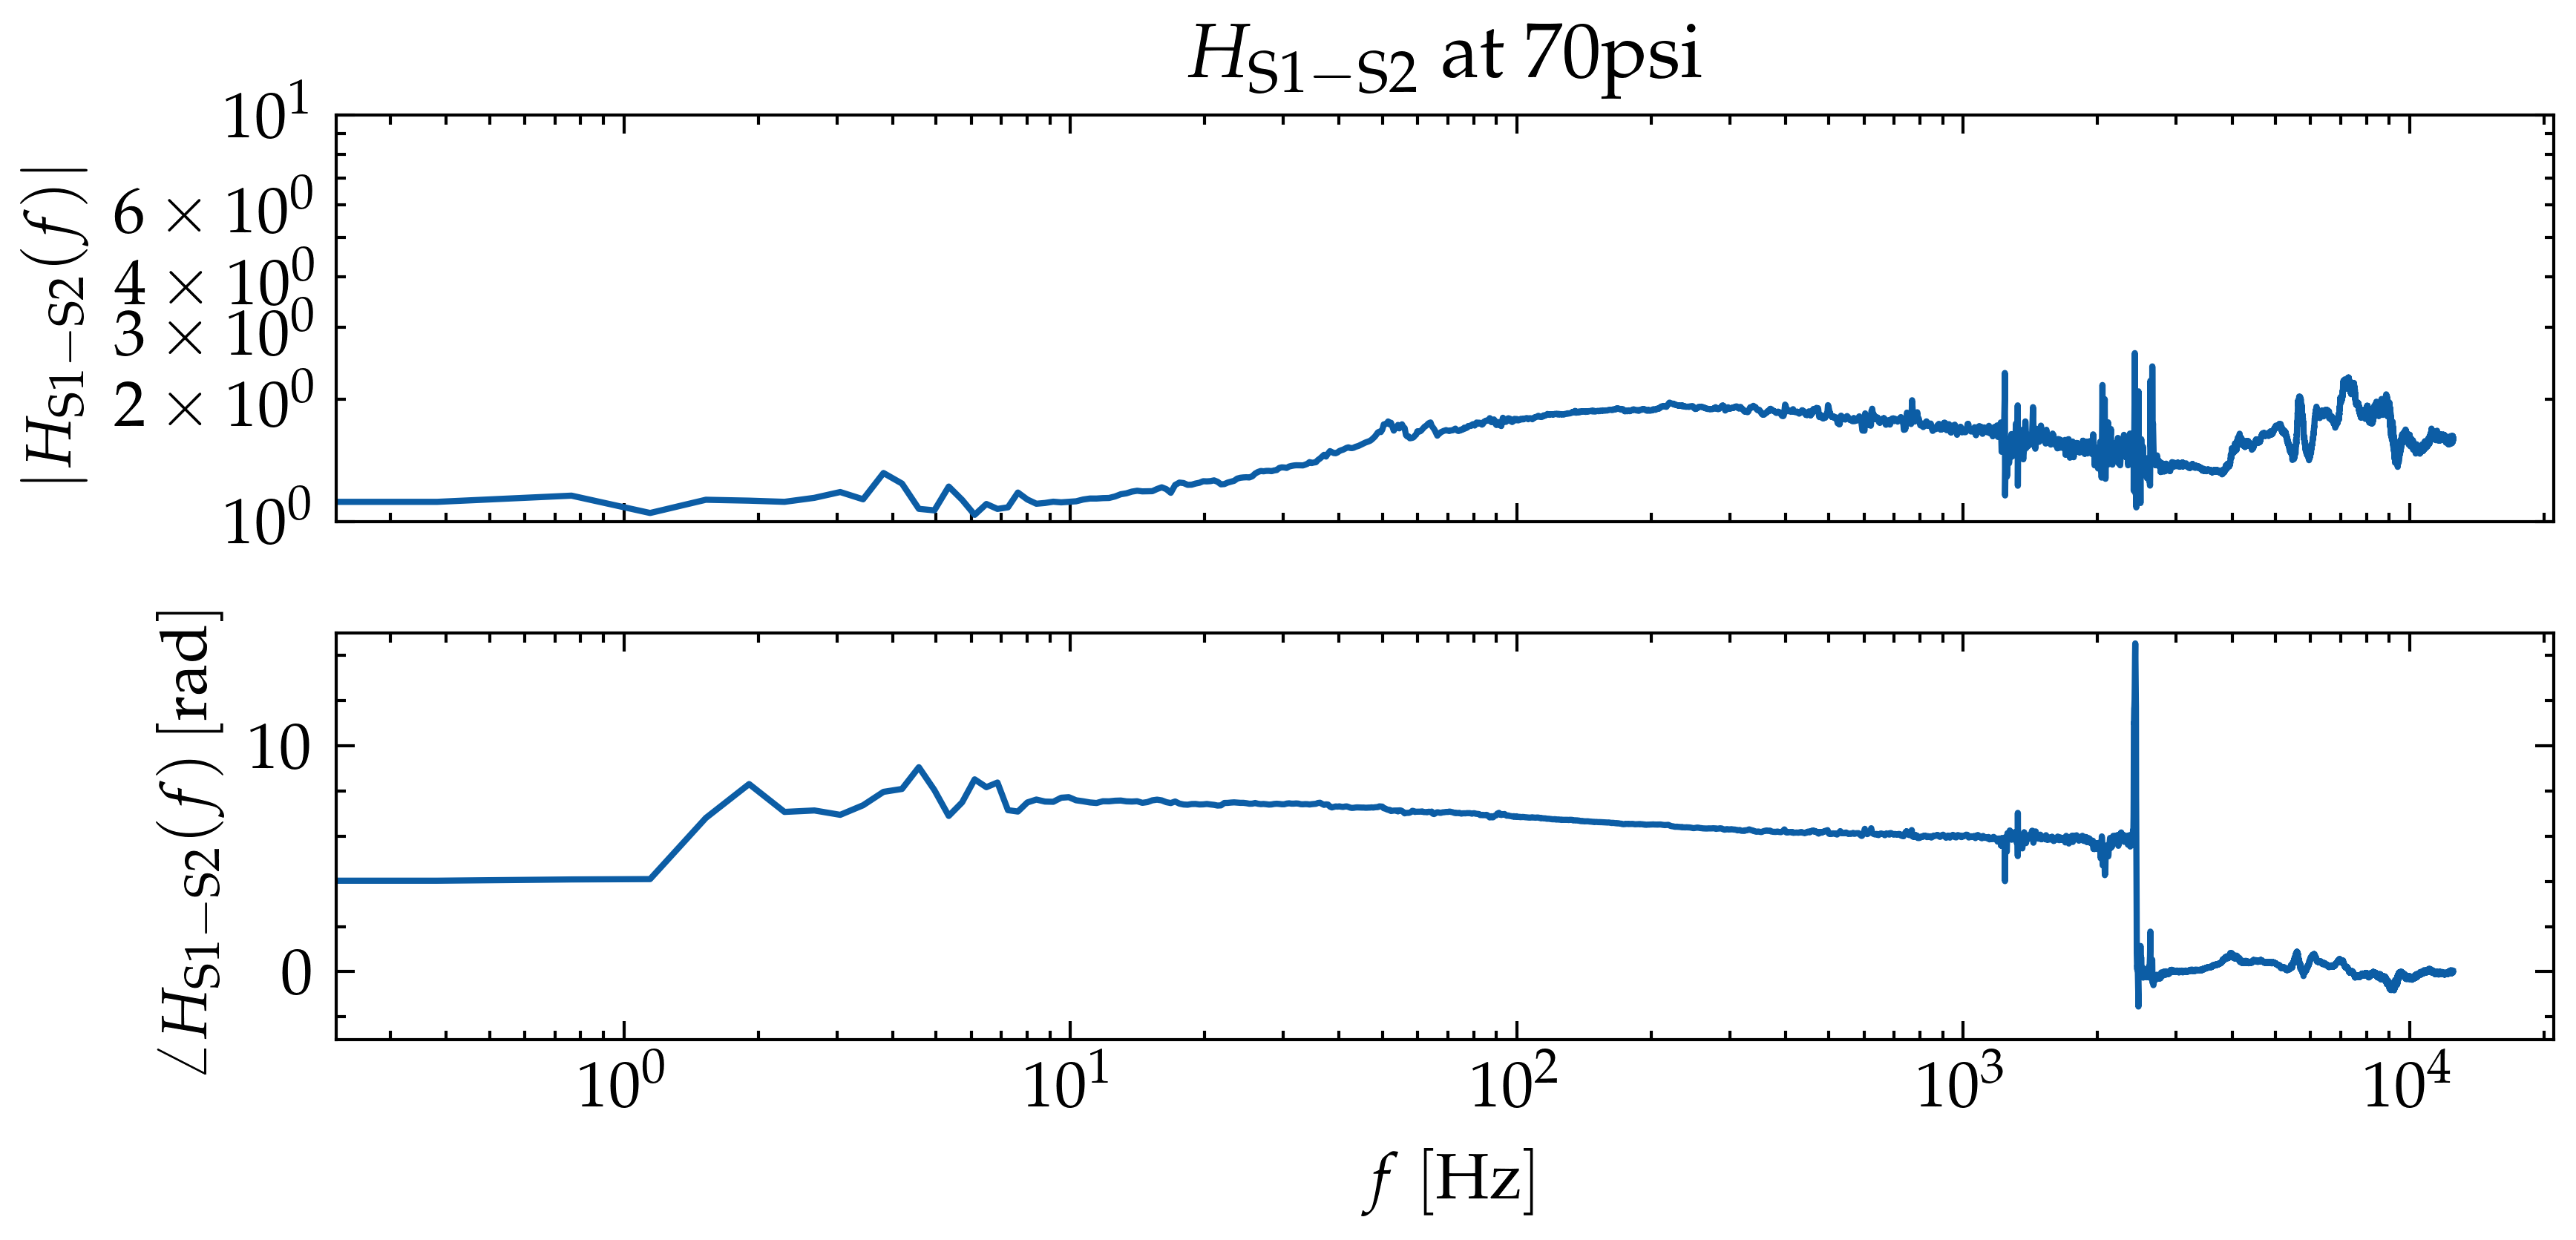
\includegraphics[width=0.8\linewidth]{S1-S2/H_70psi.png}
            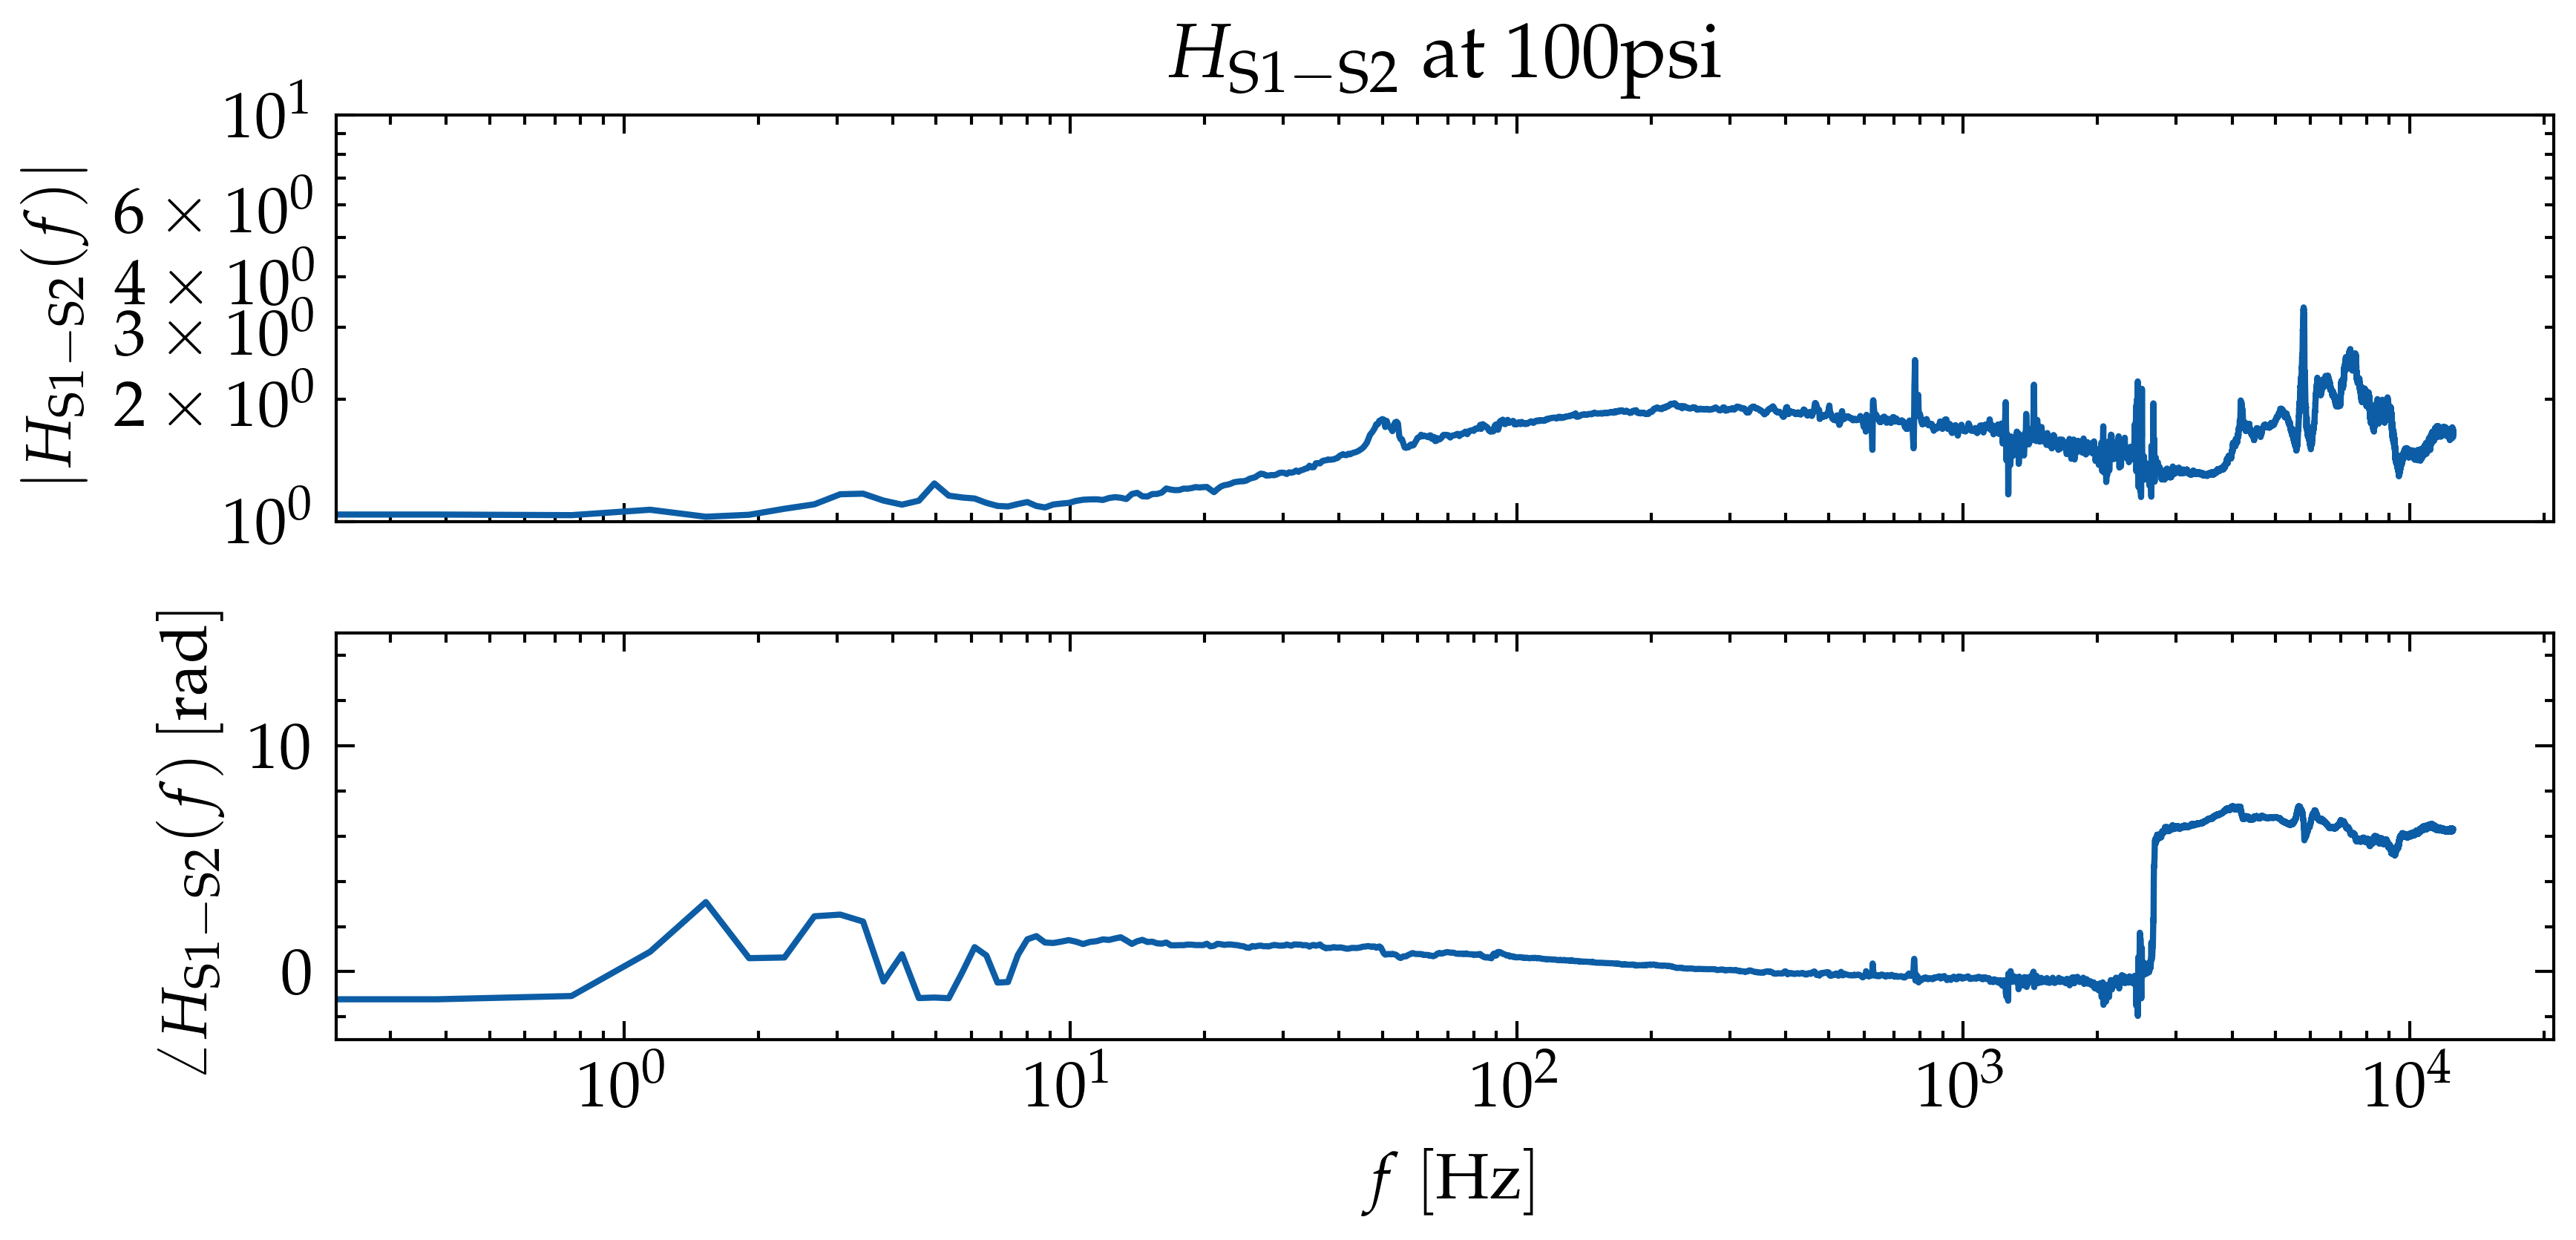
\includegraphics[width=0.8\linewidth]{S1-S2/H_100psi.png}
    \end{columns}
\end{frame}

\begin{frame}
    \frametitle{Microphone calibration: Naked (NKD)}
    \begin{columns}[c] % vertically centered
        \column{0.55\textwidth}
            \centering
            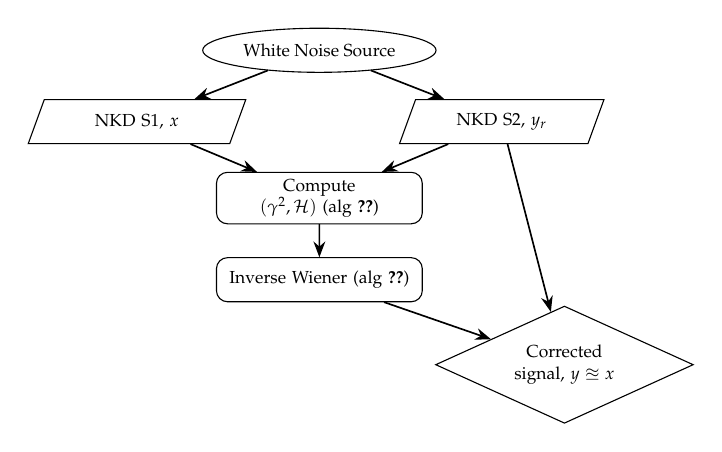
\begin{tikzpicture}[scale=0.7, transform shape,
                node distance=6mm and 18mm, every node/.style={font=\small}]
                \node (start) [terminator] {White Noise Source};

                % Two separate measurement boxes
                \node (ref)   [meas, below left = 6mm and 14mm of start, anchor=north east]
                    {NKD S1, $x$};
                \node (treat) [meas, below right = 6mm and 14mm of start, anchor=north west]
                    {NKD S2, $y_r$};

                \node (H)  [proc, below=18mm of start]
                    {Compute $(\gamma^2,\mathcal{H})$ (alg~\ref{alg:H})};

                \node (wien)  [proc, below=of H]
                    {Inverse Wiener (alg~\ref{alg:inv})};

                \node (corr)  [decision, below right = 6mm and 14mm of wien]
                    {Corrected signal, $y \approxeq x$};

                \draw [line] (start) -- (ref);
                \draw [line] (start) -- (treat);
                \draw [line] (ref) -- (H);
                \draw [line] (treat) -- (H);
                \draw [line] (H) -- (wien);
                \draw [line] (wien) -- (corr);
                \draw [line] (treat) -- (corr);

            \end{tikzpicture}
        \column{0.4\textwidth}
            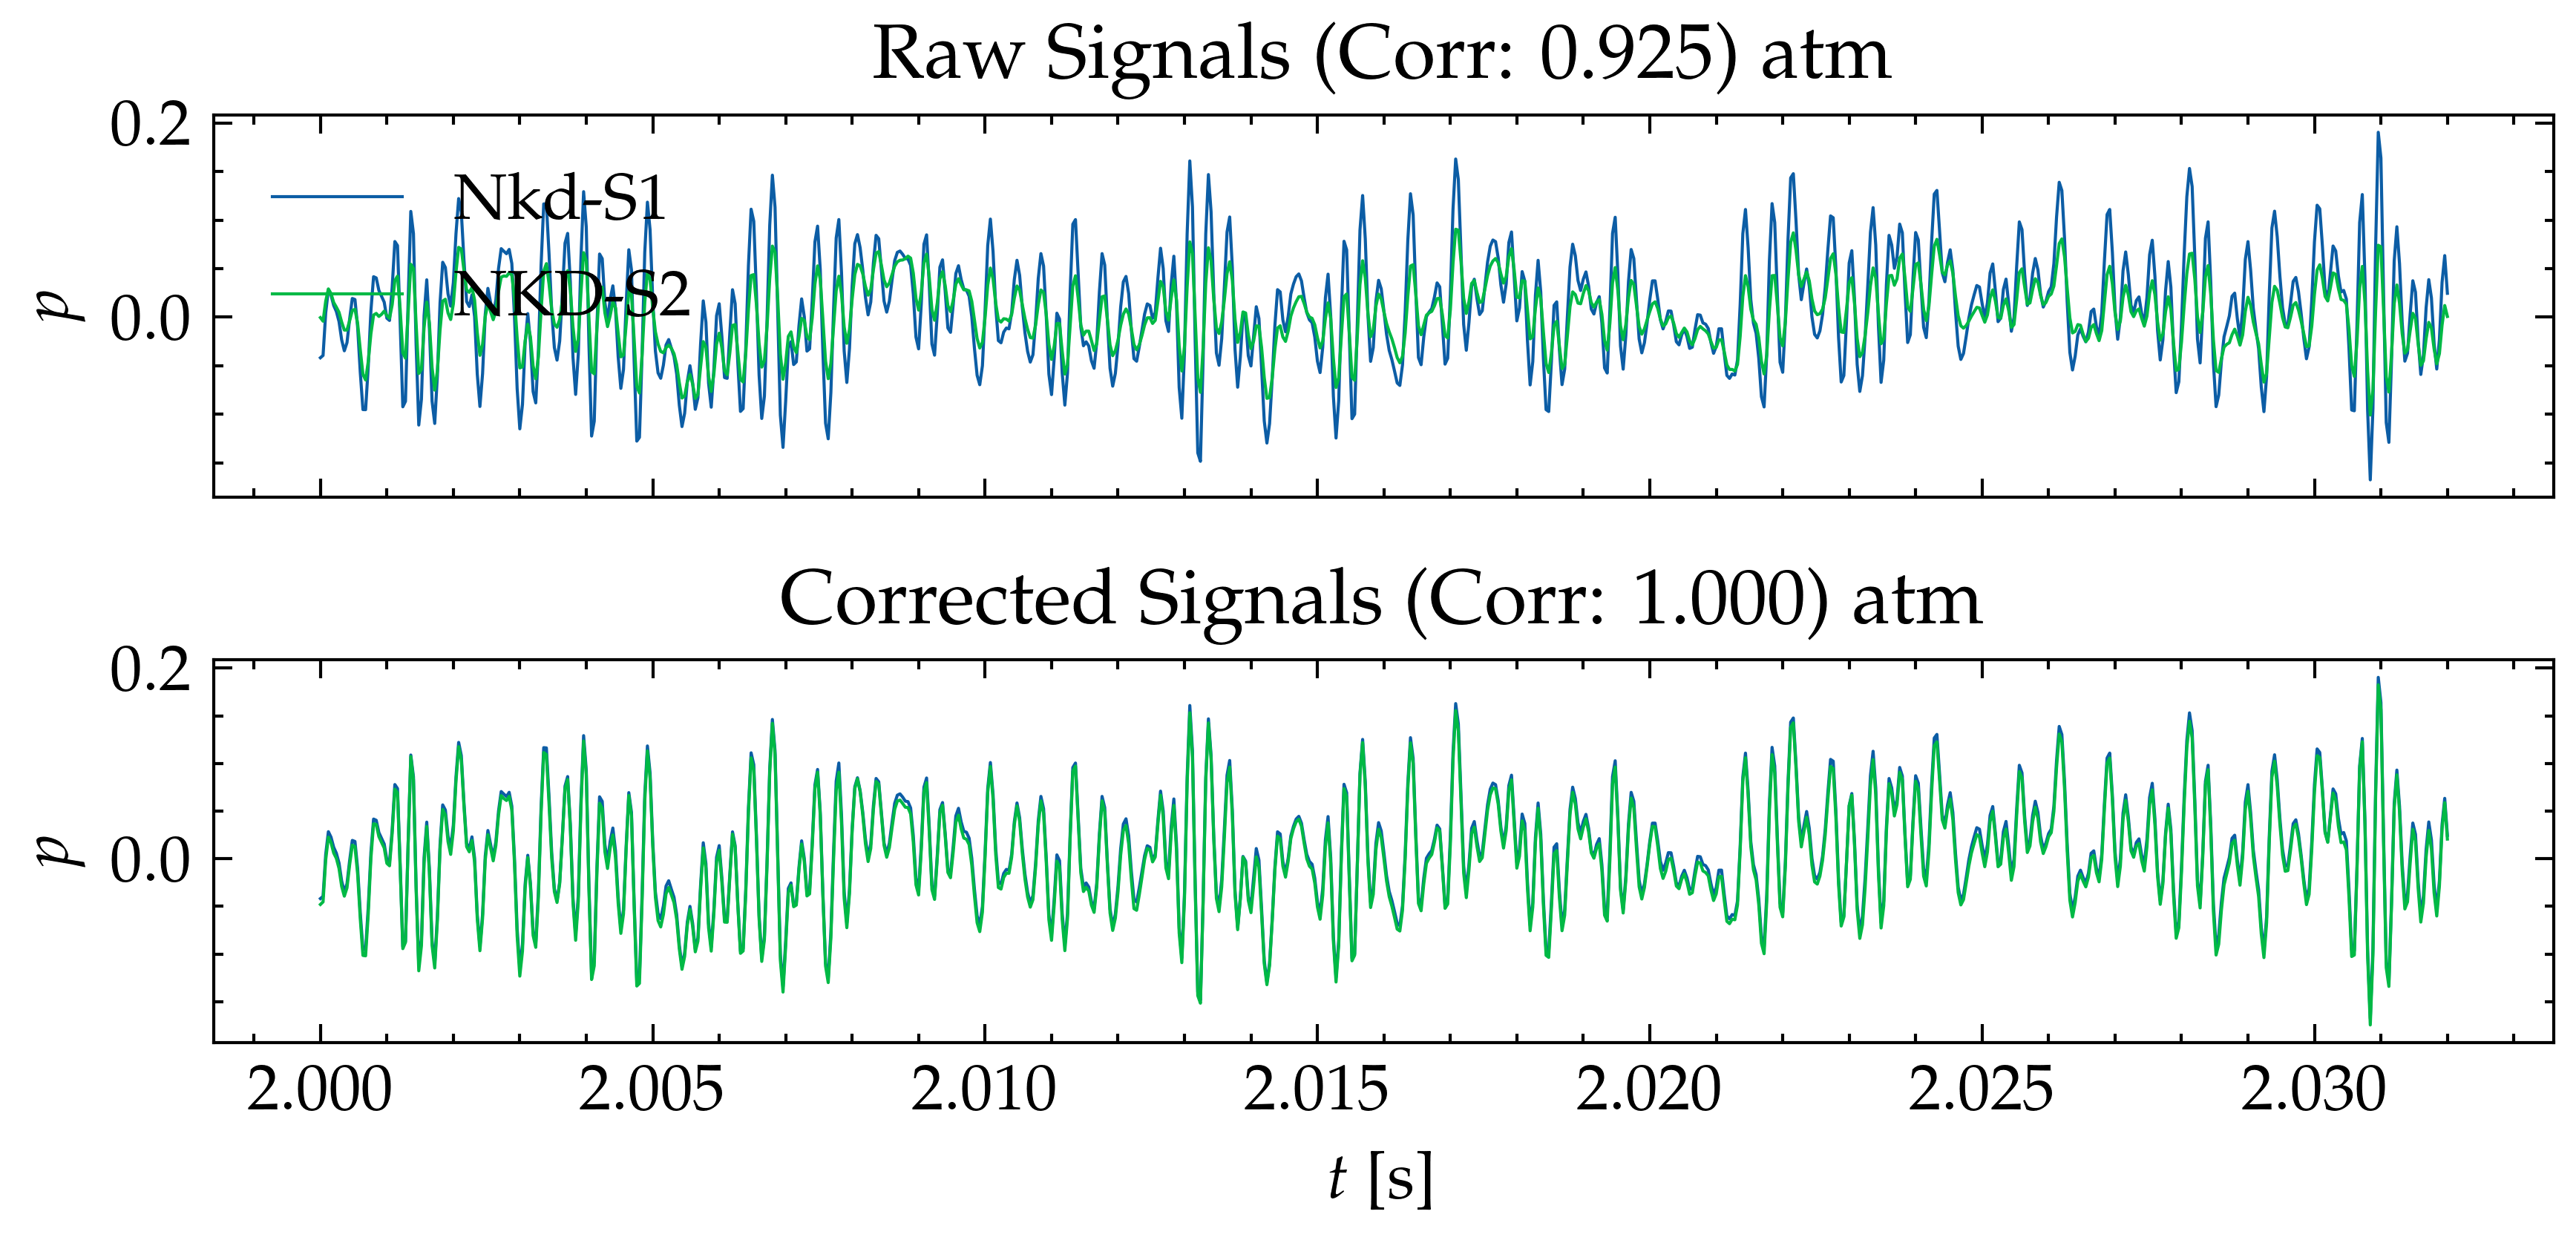
\includegraphics[width=0.8\linewidth]{S1-S2/y_atm.png}
            % 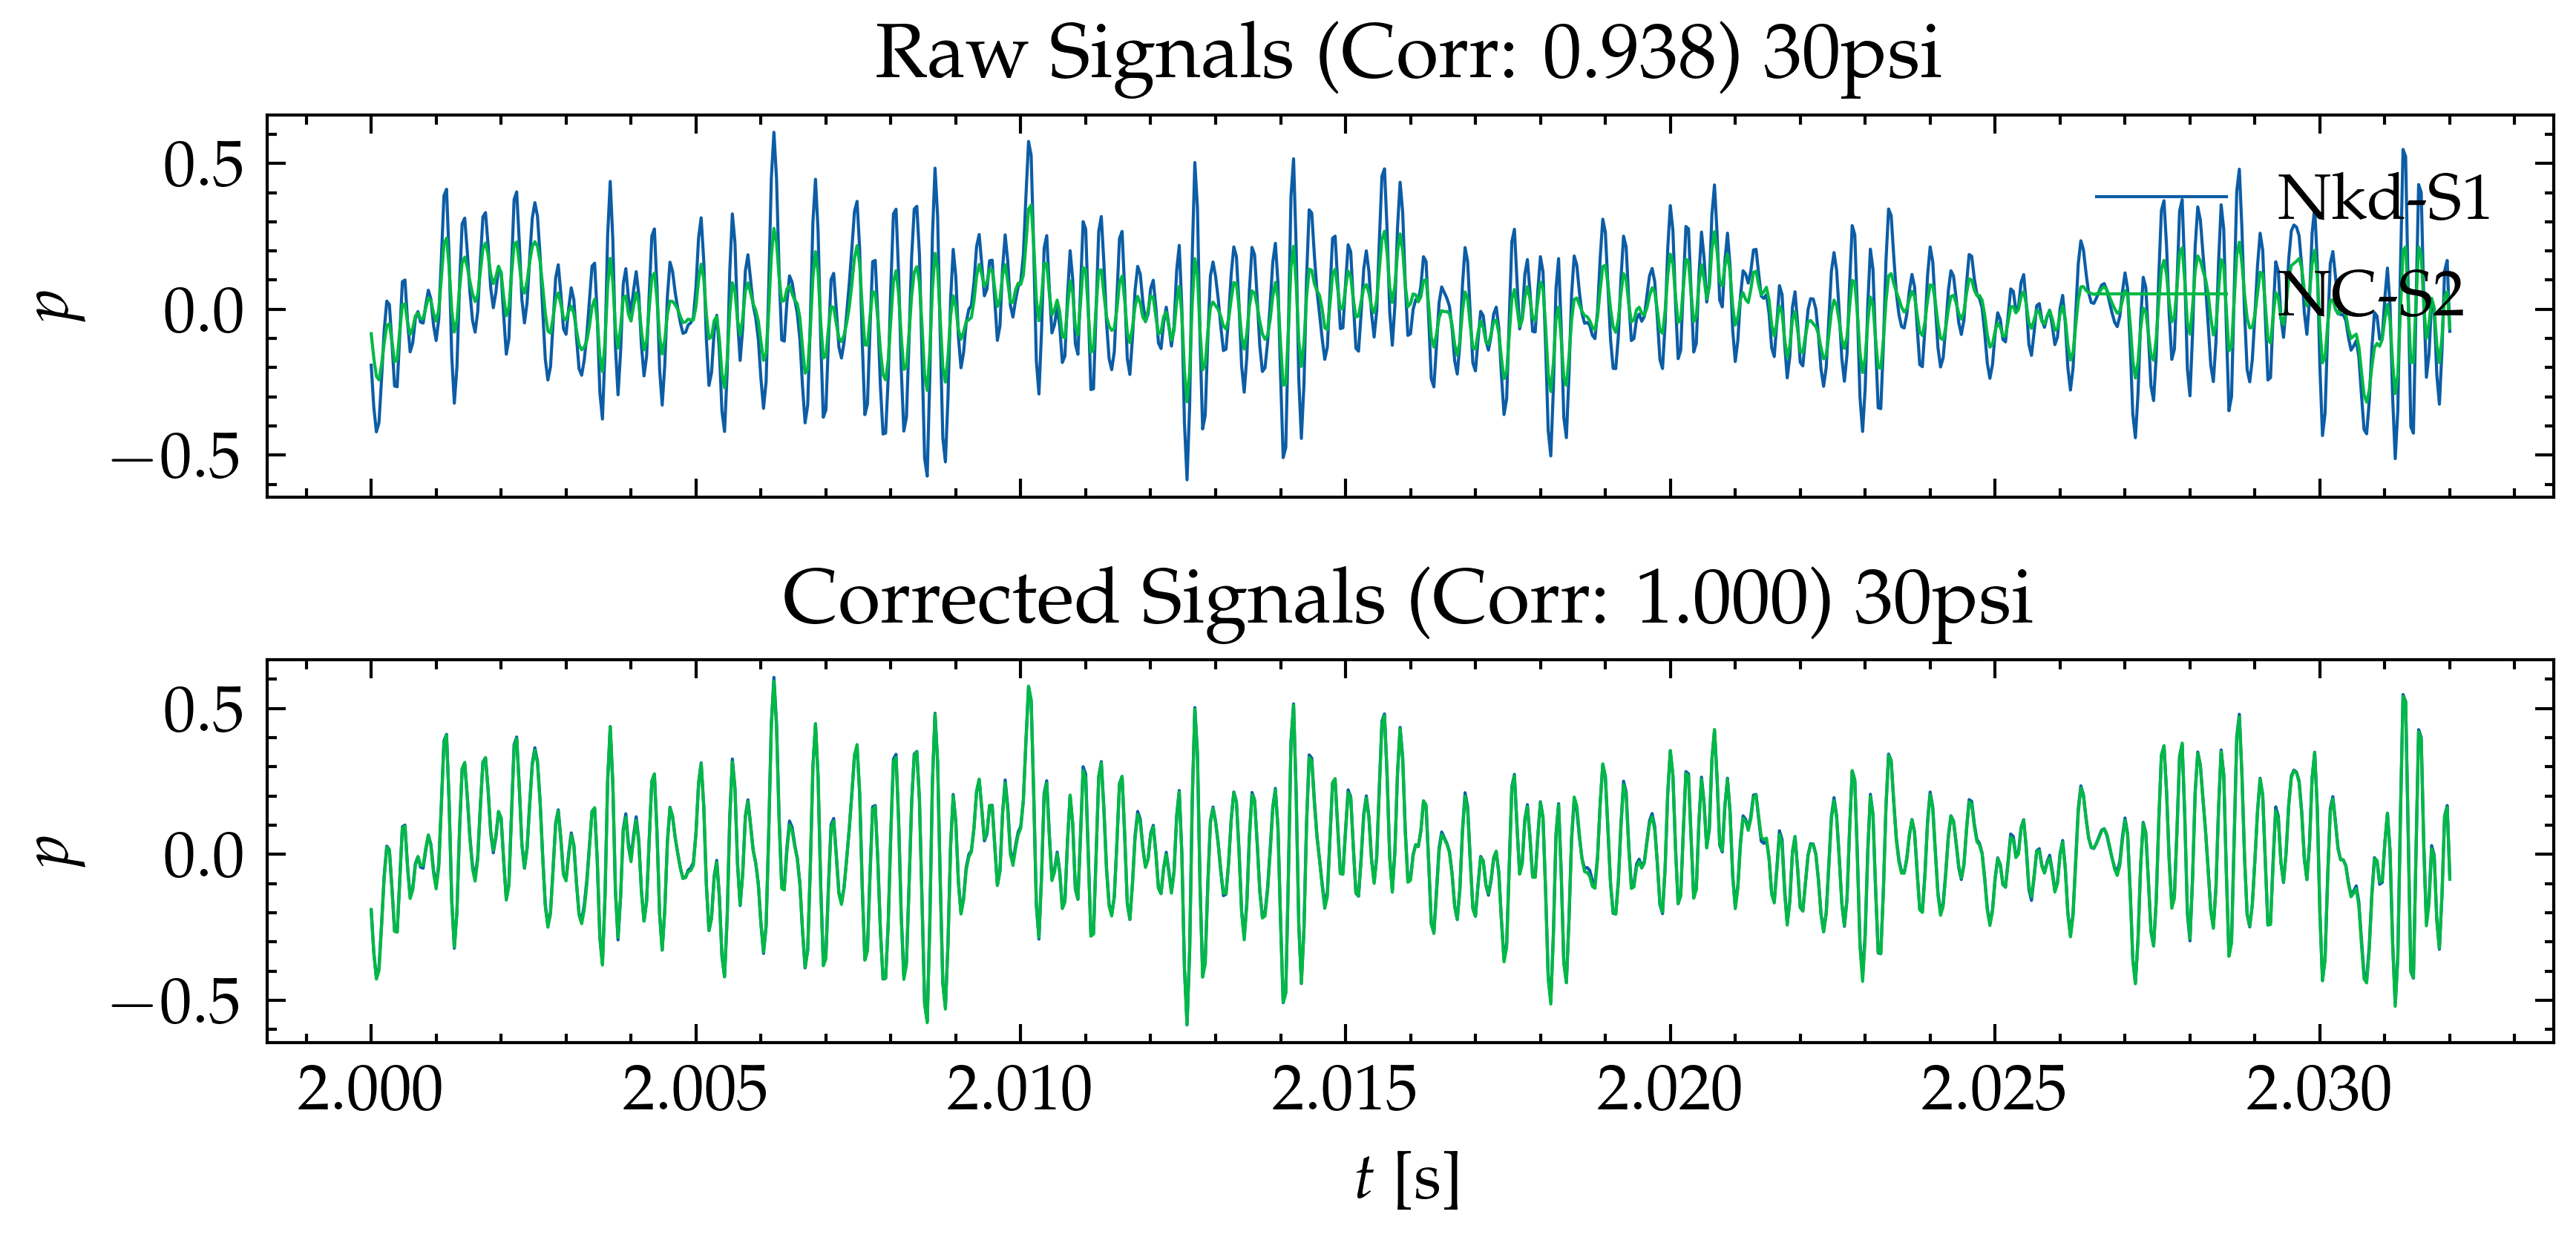
\includegraphics[width=0.8\linewidth]{S1-S2/y_30psi.png}
            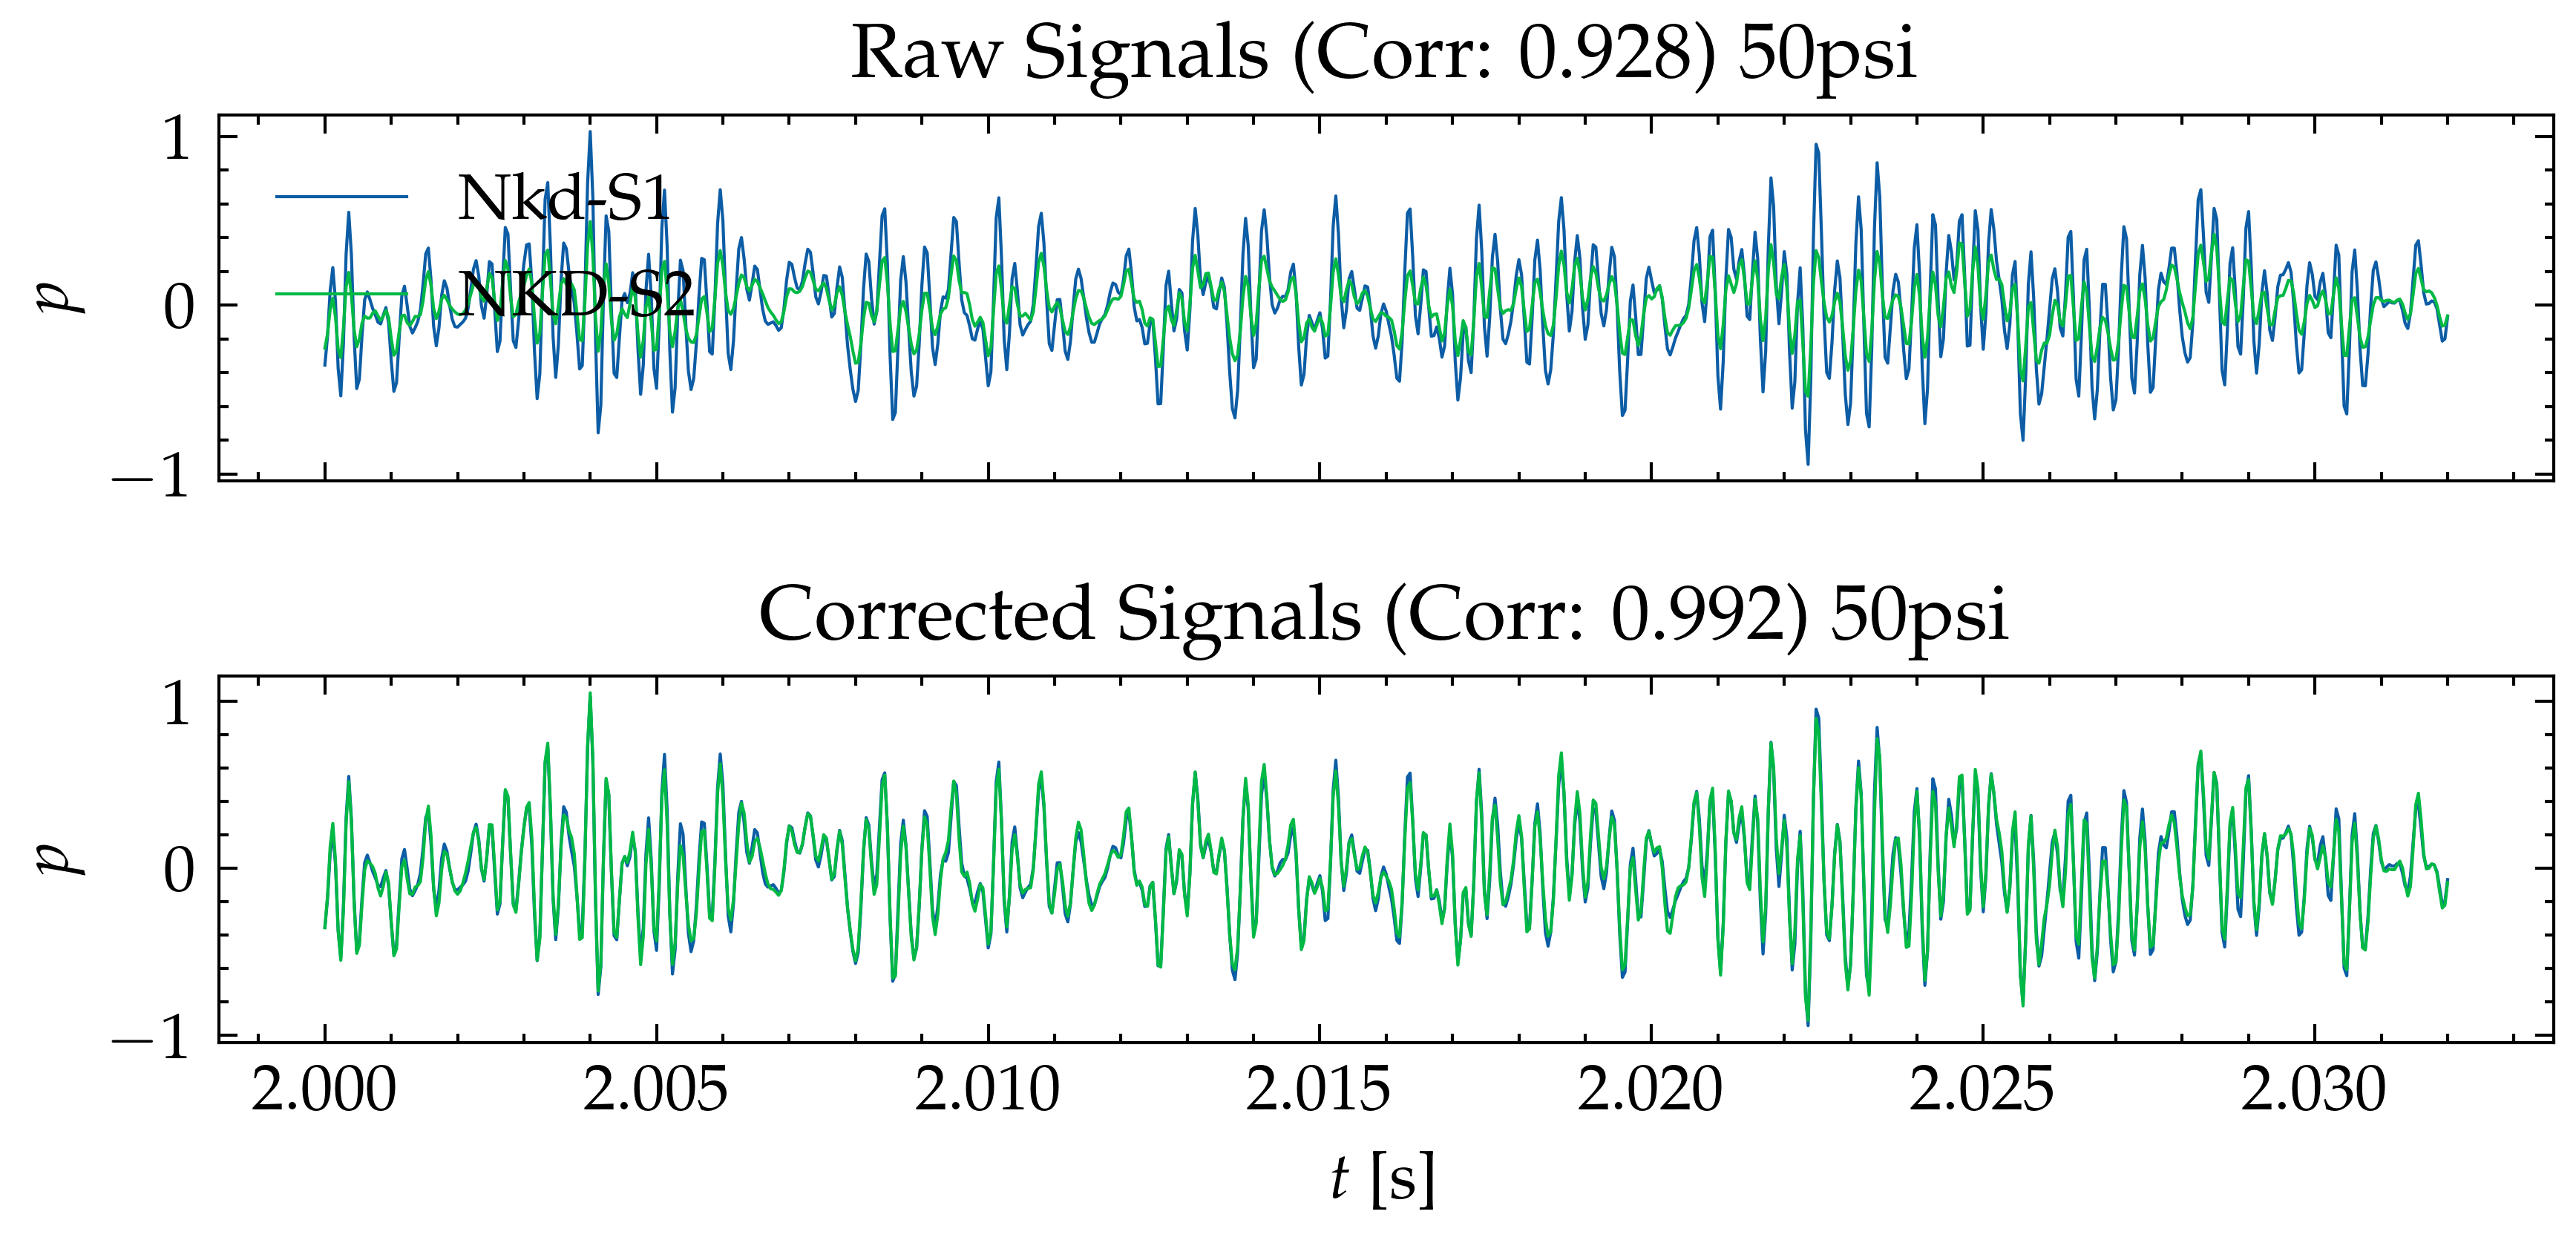
\includegraphics[width=0.8\linewidth]{S1-S2/y_50psi.png}
            % 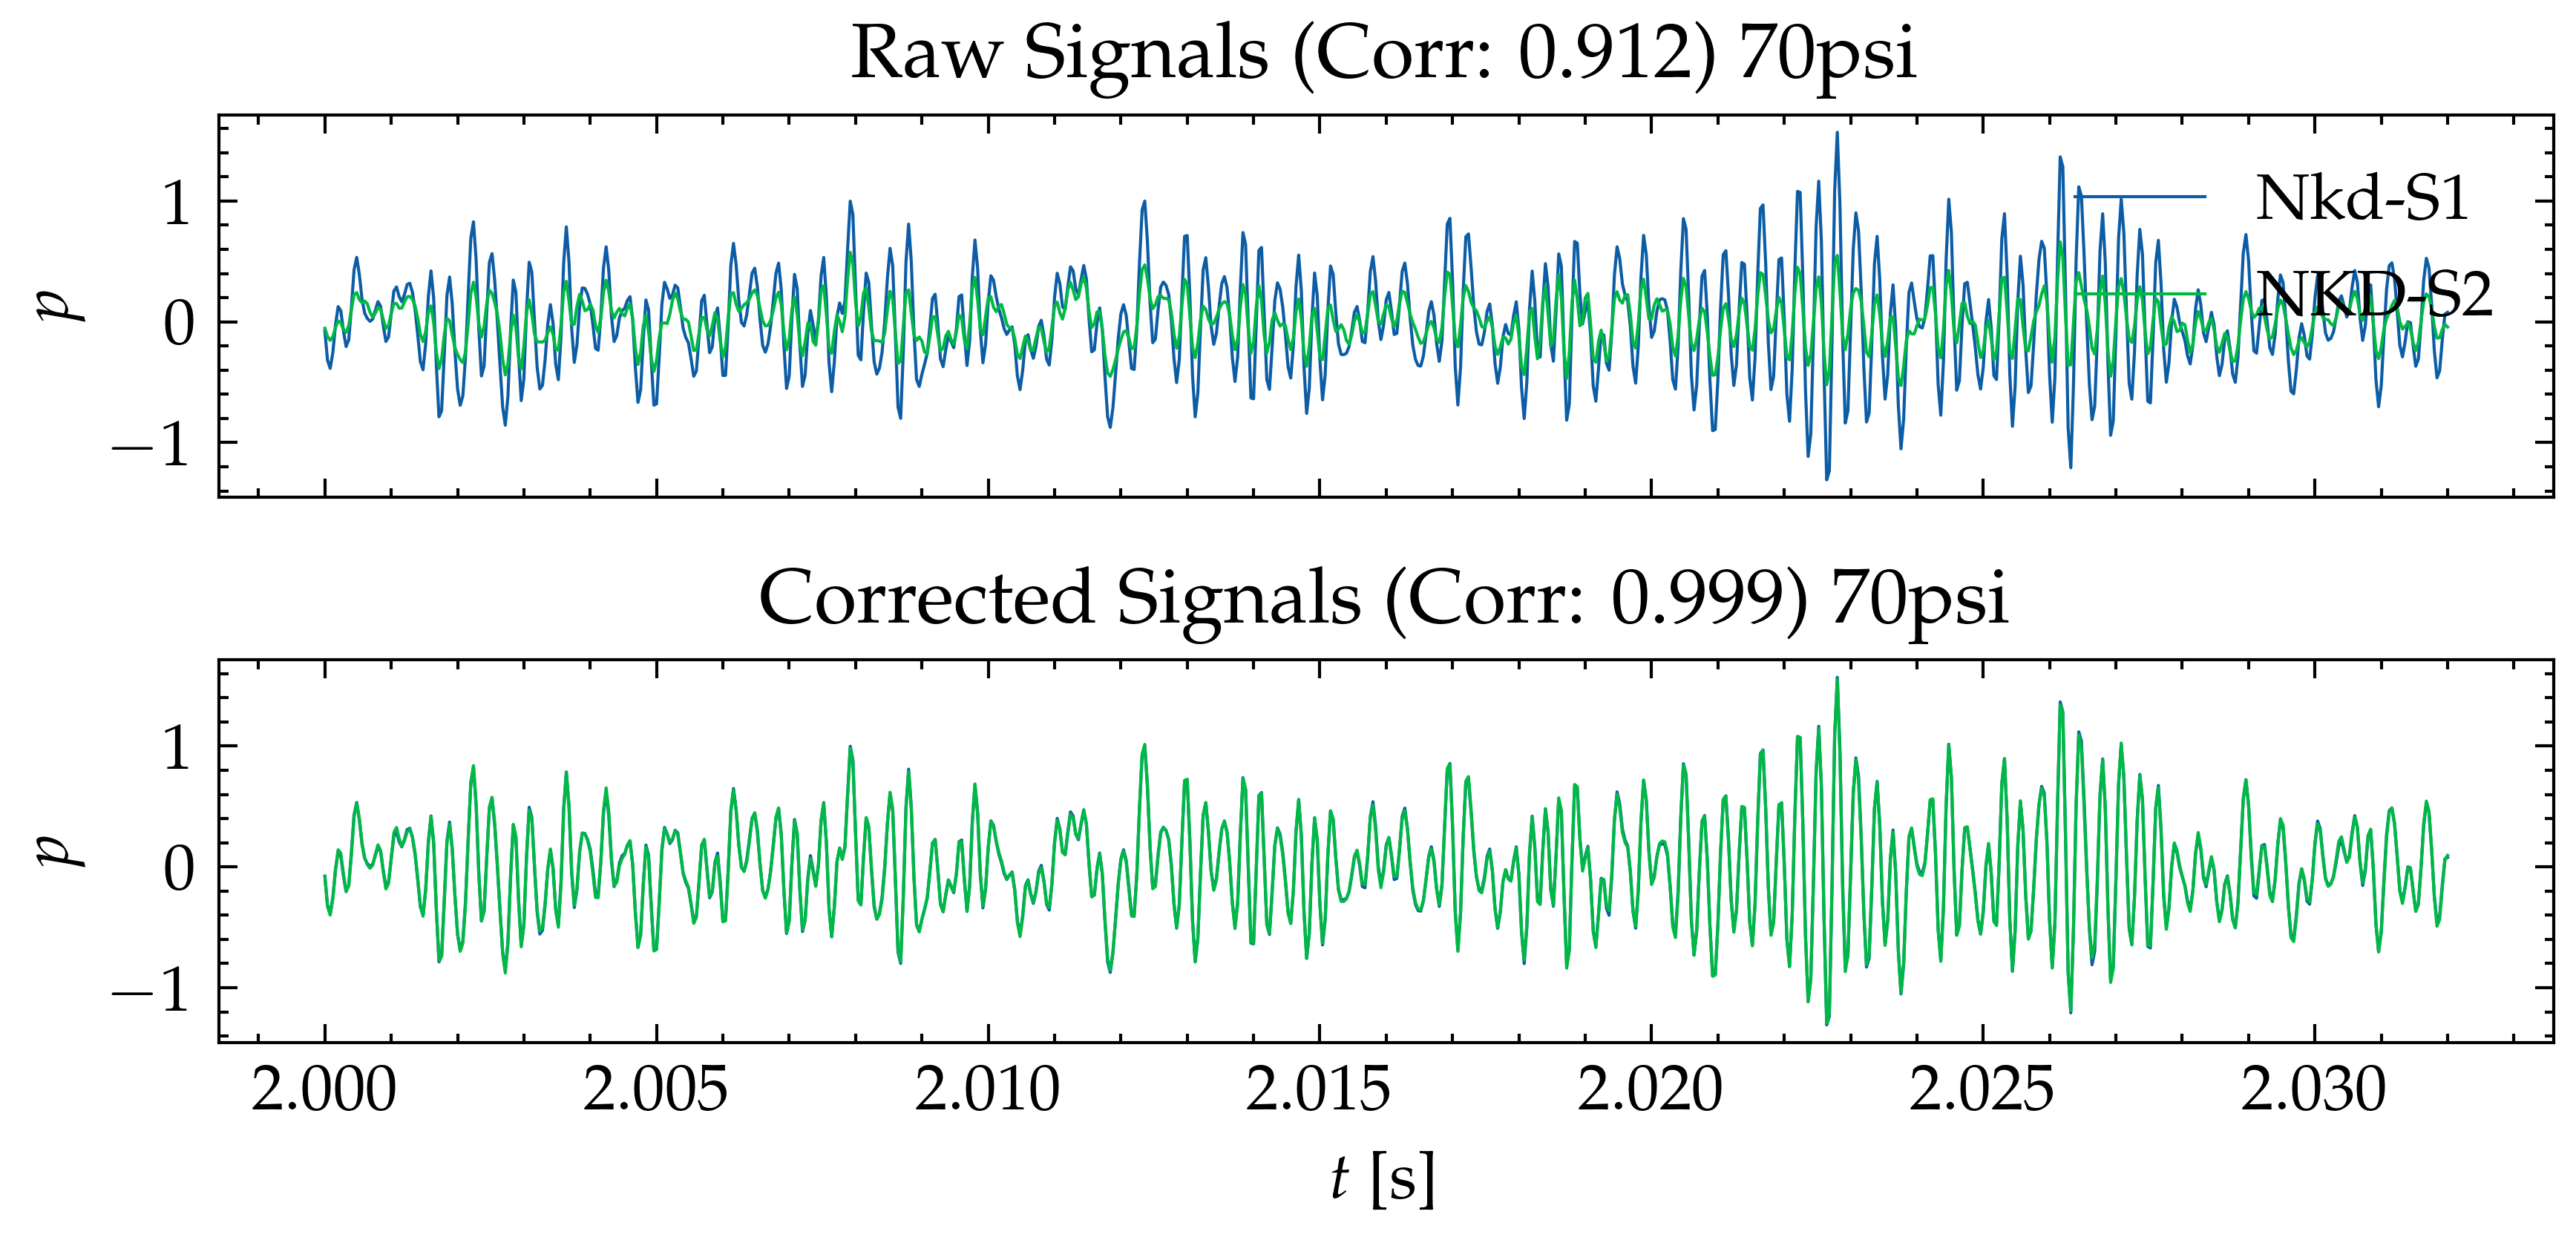
\includegraphics[width=0.8\linewidth]{S1-S2/y_70psi.png}
            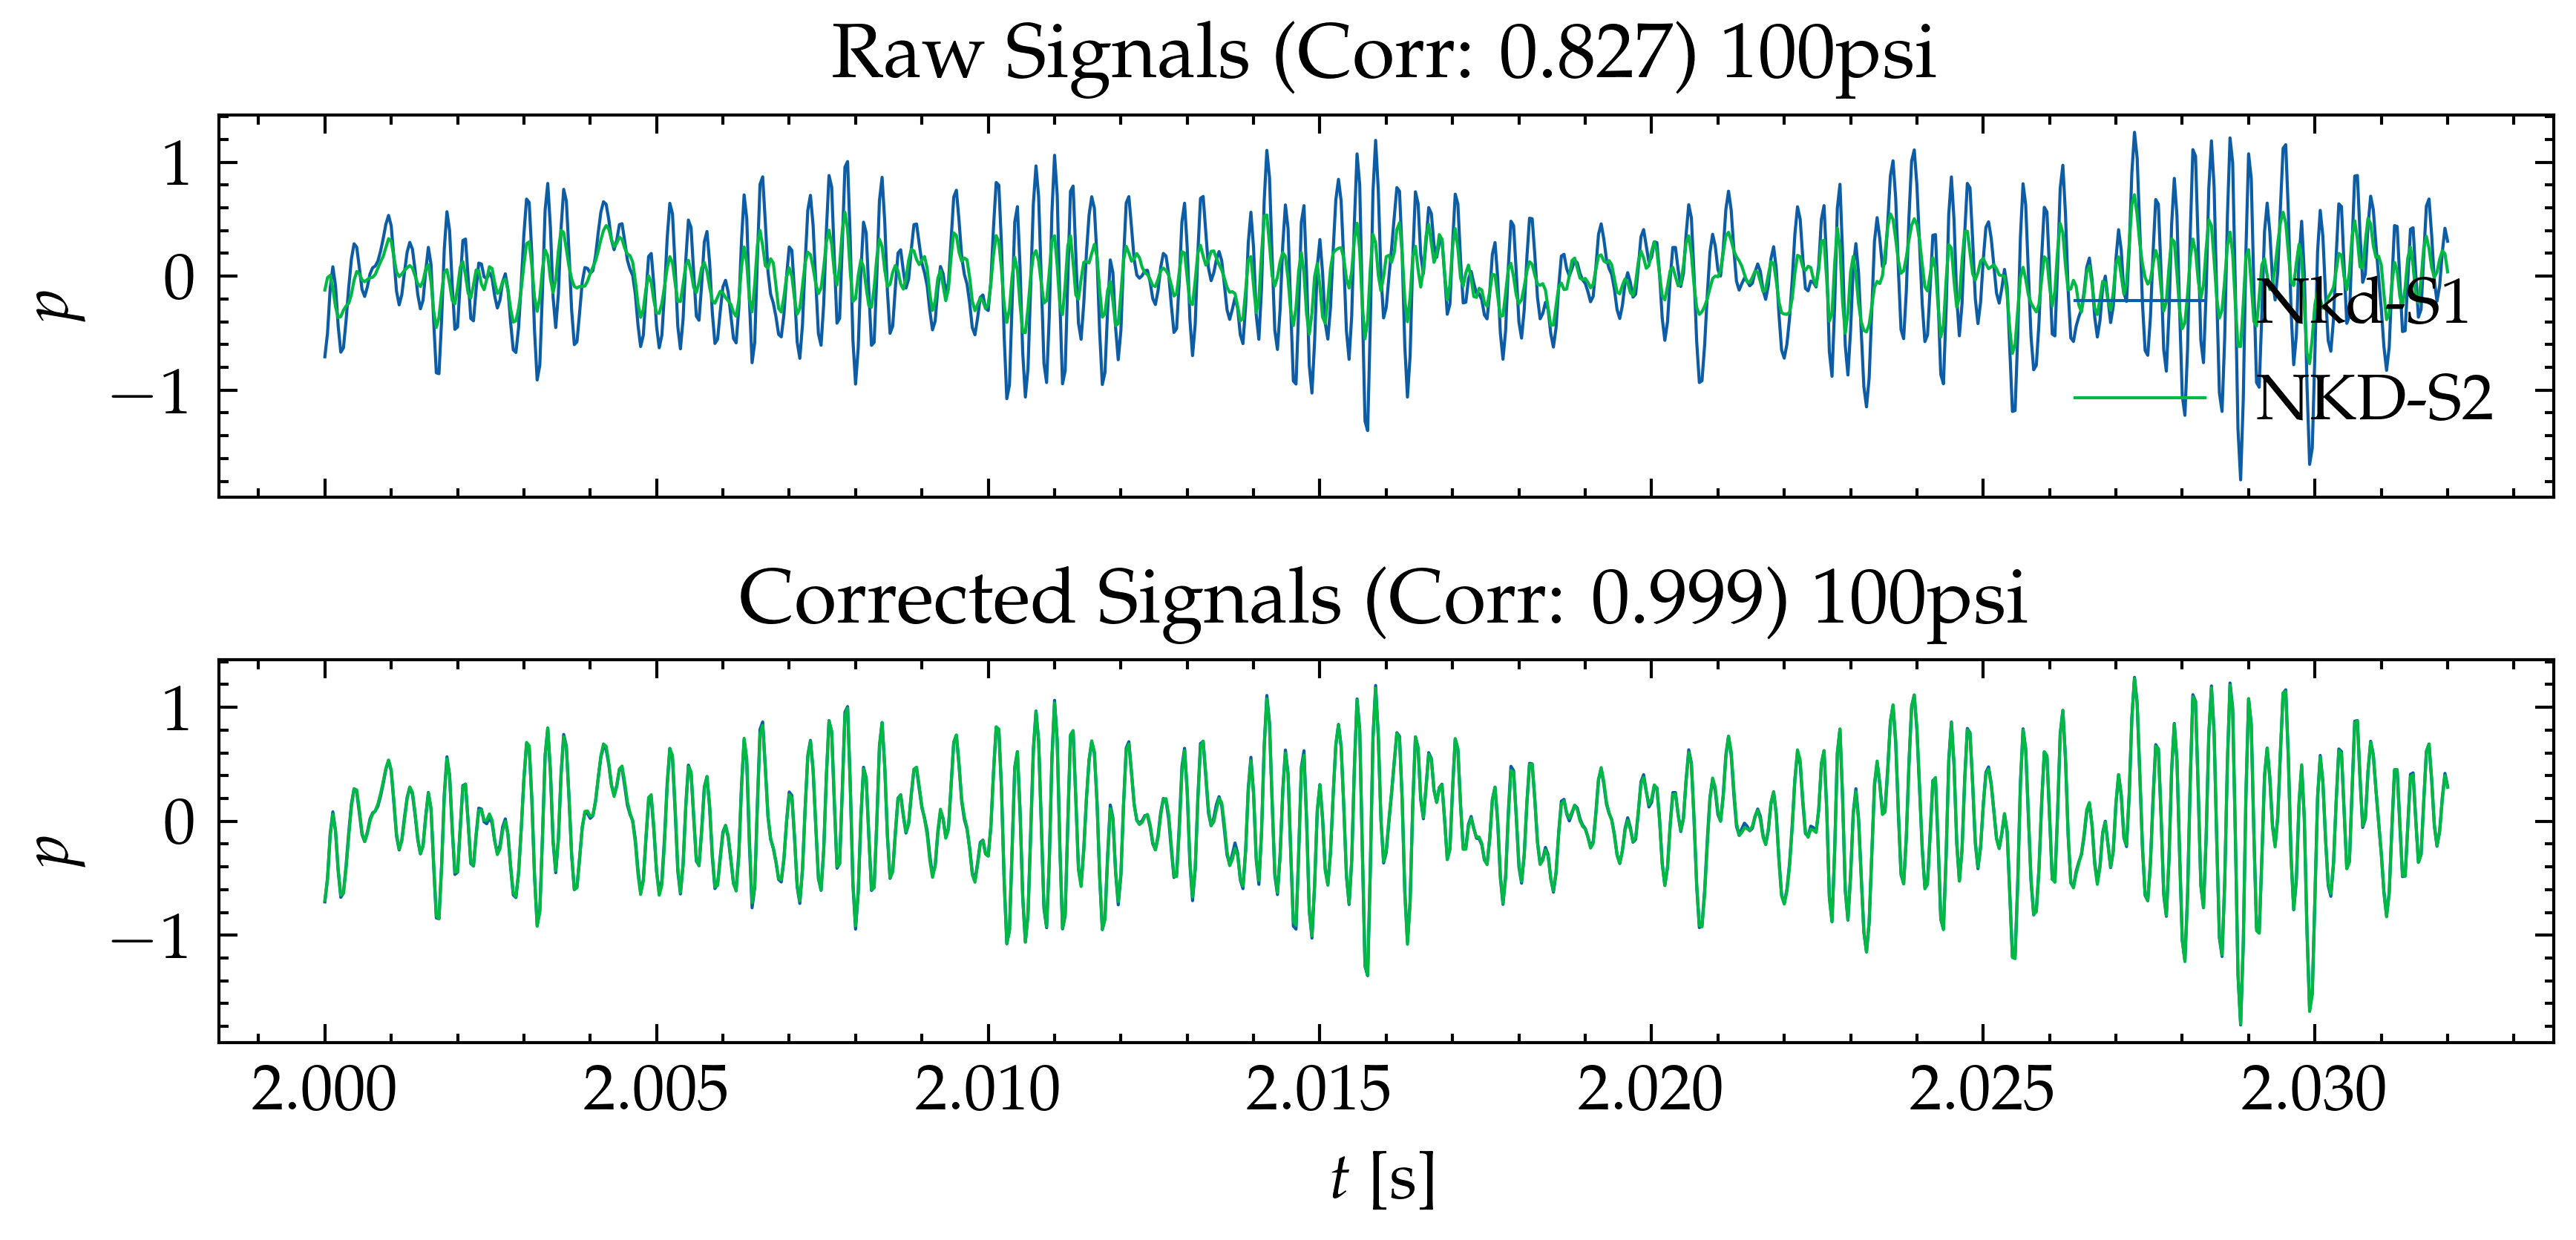
\includegraphics[width=0.8\linewidth]{S1-S2/y_100psi.png}
    \end{columns}
\end{frame}

\begin{frame}
    \frametitle{Microphone calibration: Nose Cone (NC)}
    \begin{columns}[c] % vertically centered
        \column{0.55\textwidth}
            \centering
            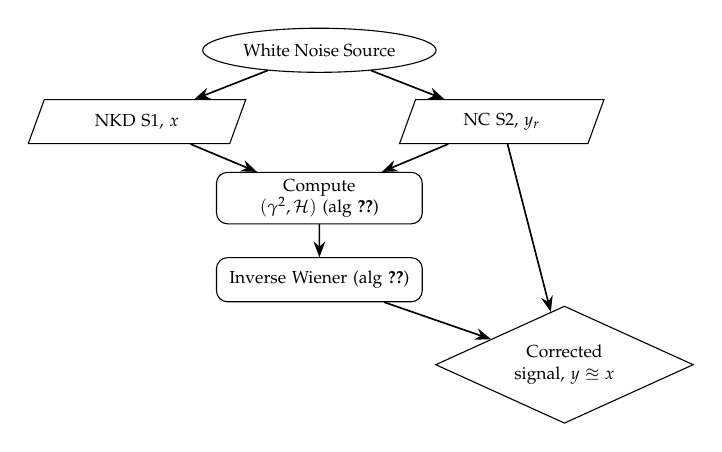
\begin{tikzpicture}[scale=0.7, transform shape,
                node distance=6mm and 18mm, every node/.style={font=\small}]
                \node (start) [terminator] {White Noise Source};

                % Two separate measurement boxes
                \node (ref)   [meas, below left = 6mm and 14mm of start, anchor=north east]
                    {NKD S1, $x$};
                \node (treat) [meas, below right = 6mm and 14mm of start, anchor=north west]
                    {NC S2, $y_r$};

                \node (H)  [proc, below=18mm of start]
                    {Compute $(\gamma^2,\mathcal{H})$ (alg~\ref{alg:H})};

                \node (wien)  [proc, below=of H]
                    {Inverse Wiener (alg~\ref{alg:inv})};

                \node (corr)  [decision, below right = 6mm and 14mm of wien]
                    {Corrected signal, $y \approxeq x$};

                \draw [line] (start) -- (ref);
                \draw [line] (start) -- (treat);
                \draw [line] (ref) -- (H);
                \draw [line] (treat) -- (H);
                \draw [line] (H) -- (wien);
                \draw [line] (wien) -- (corr);
                \draw [line] (treat) -- (corr);

            \end{tikzpicture}
        \column{0.4\textwidth}
            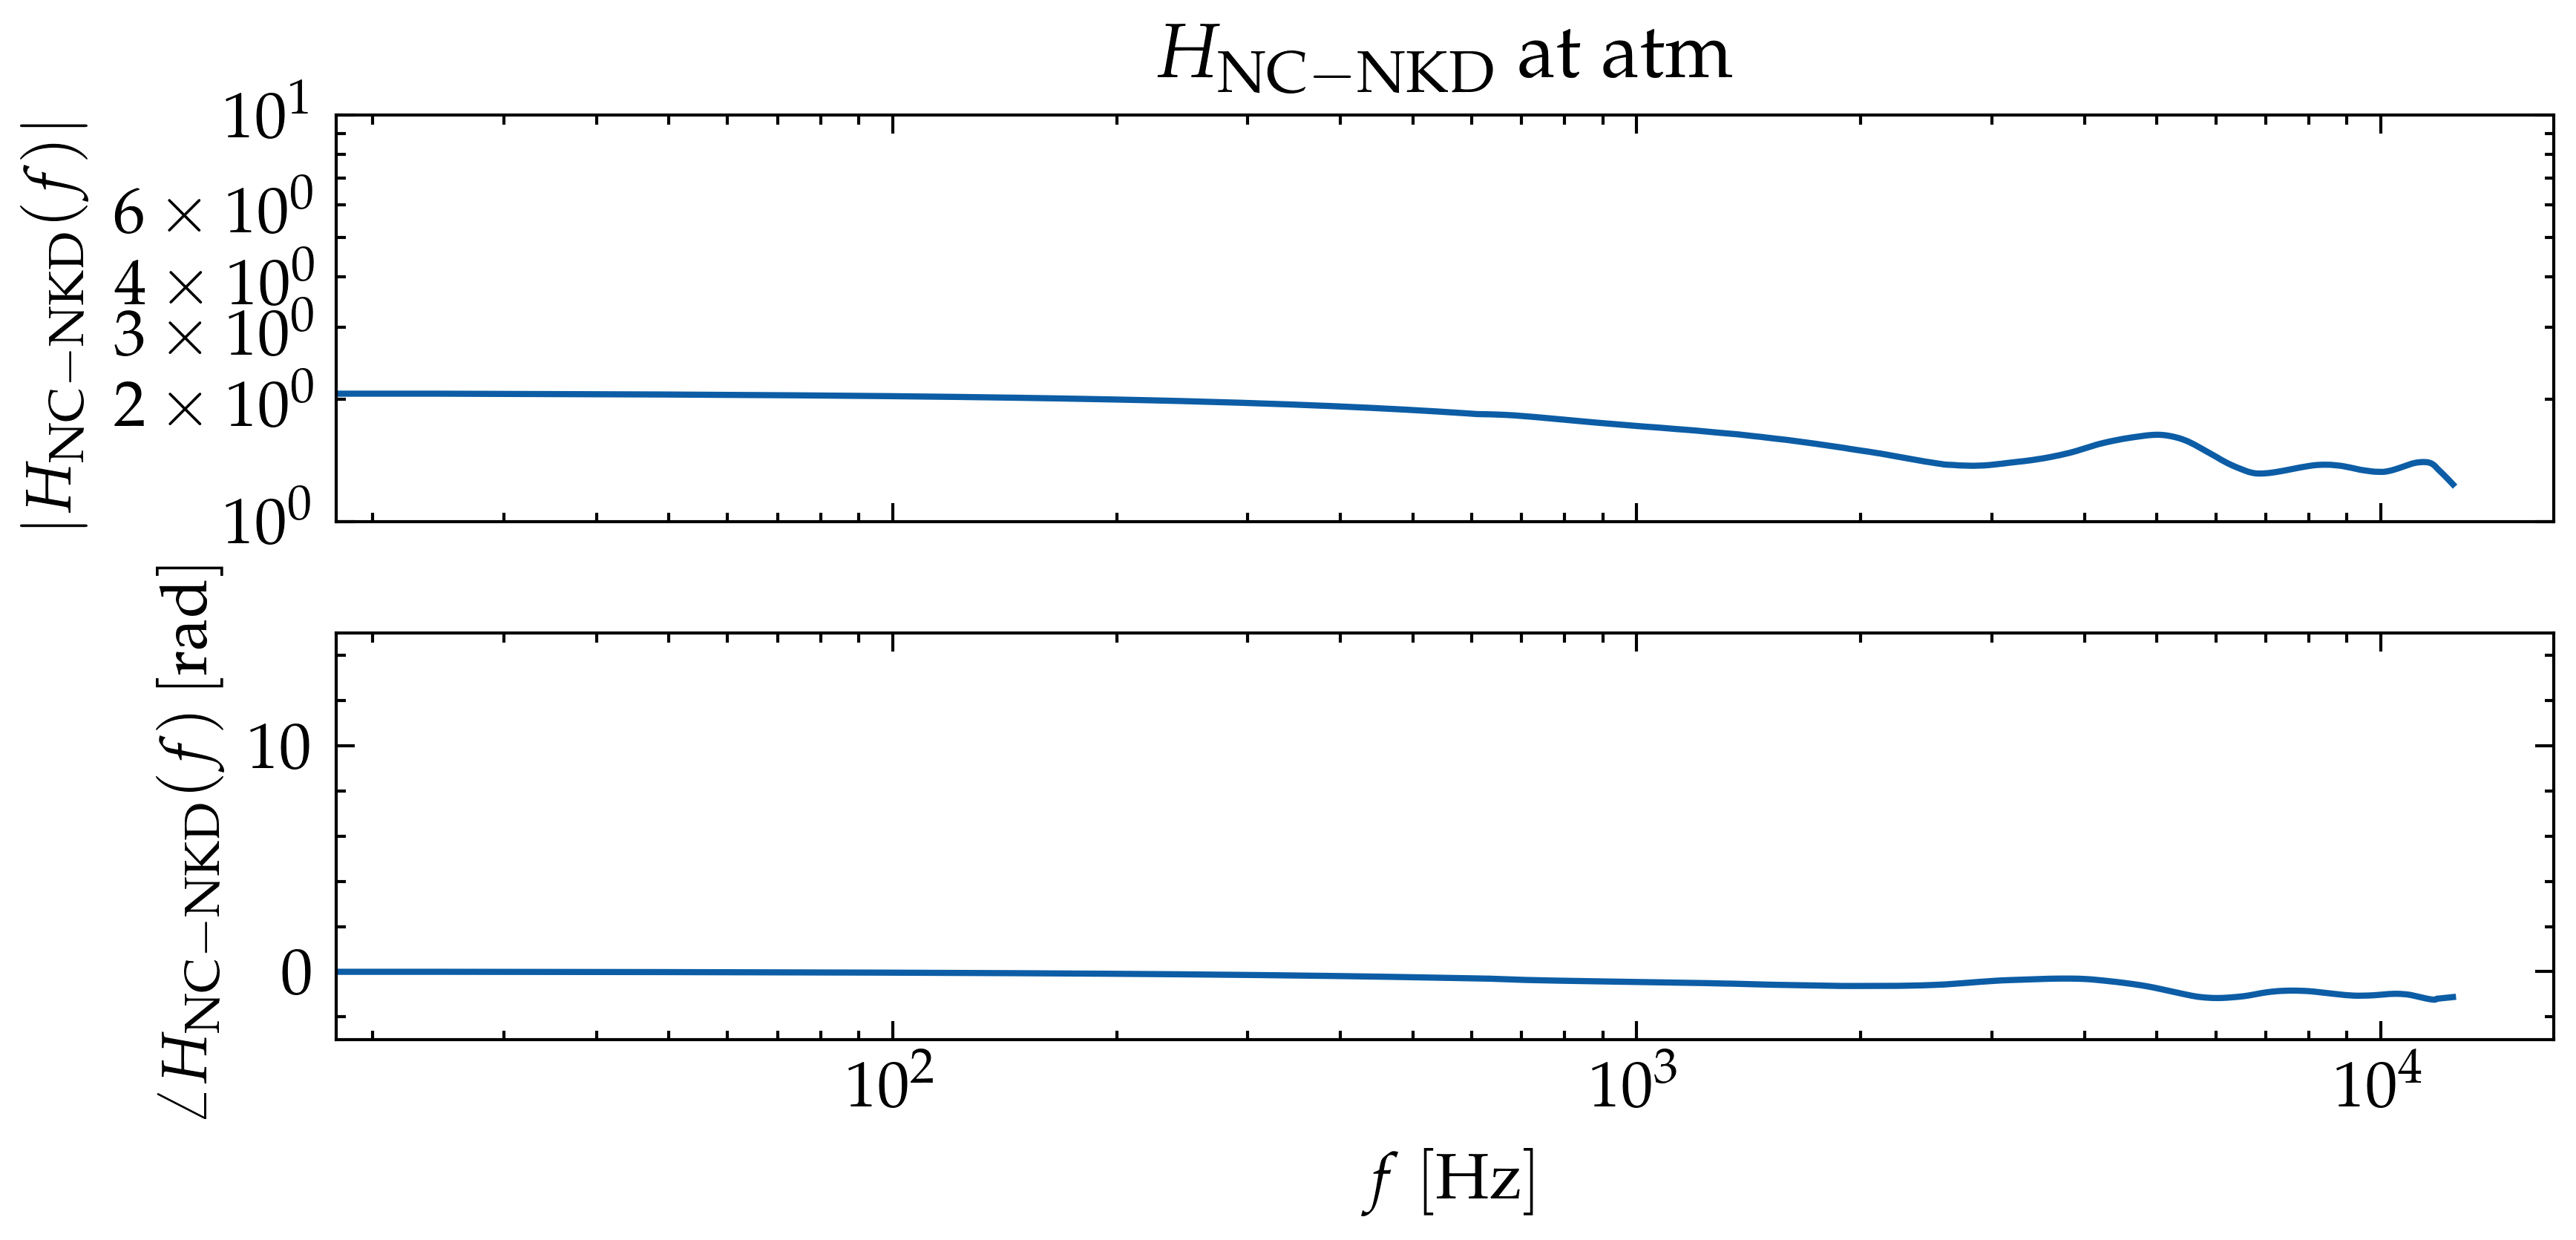
\includegraphics[width=0.8\linewidth]{NC-NKD/H_atm.png}
            % 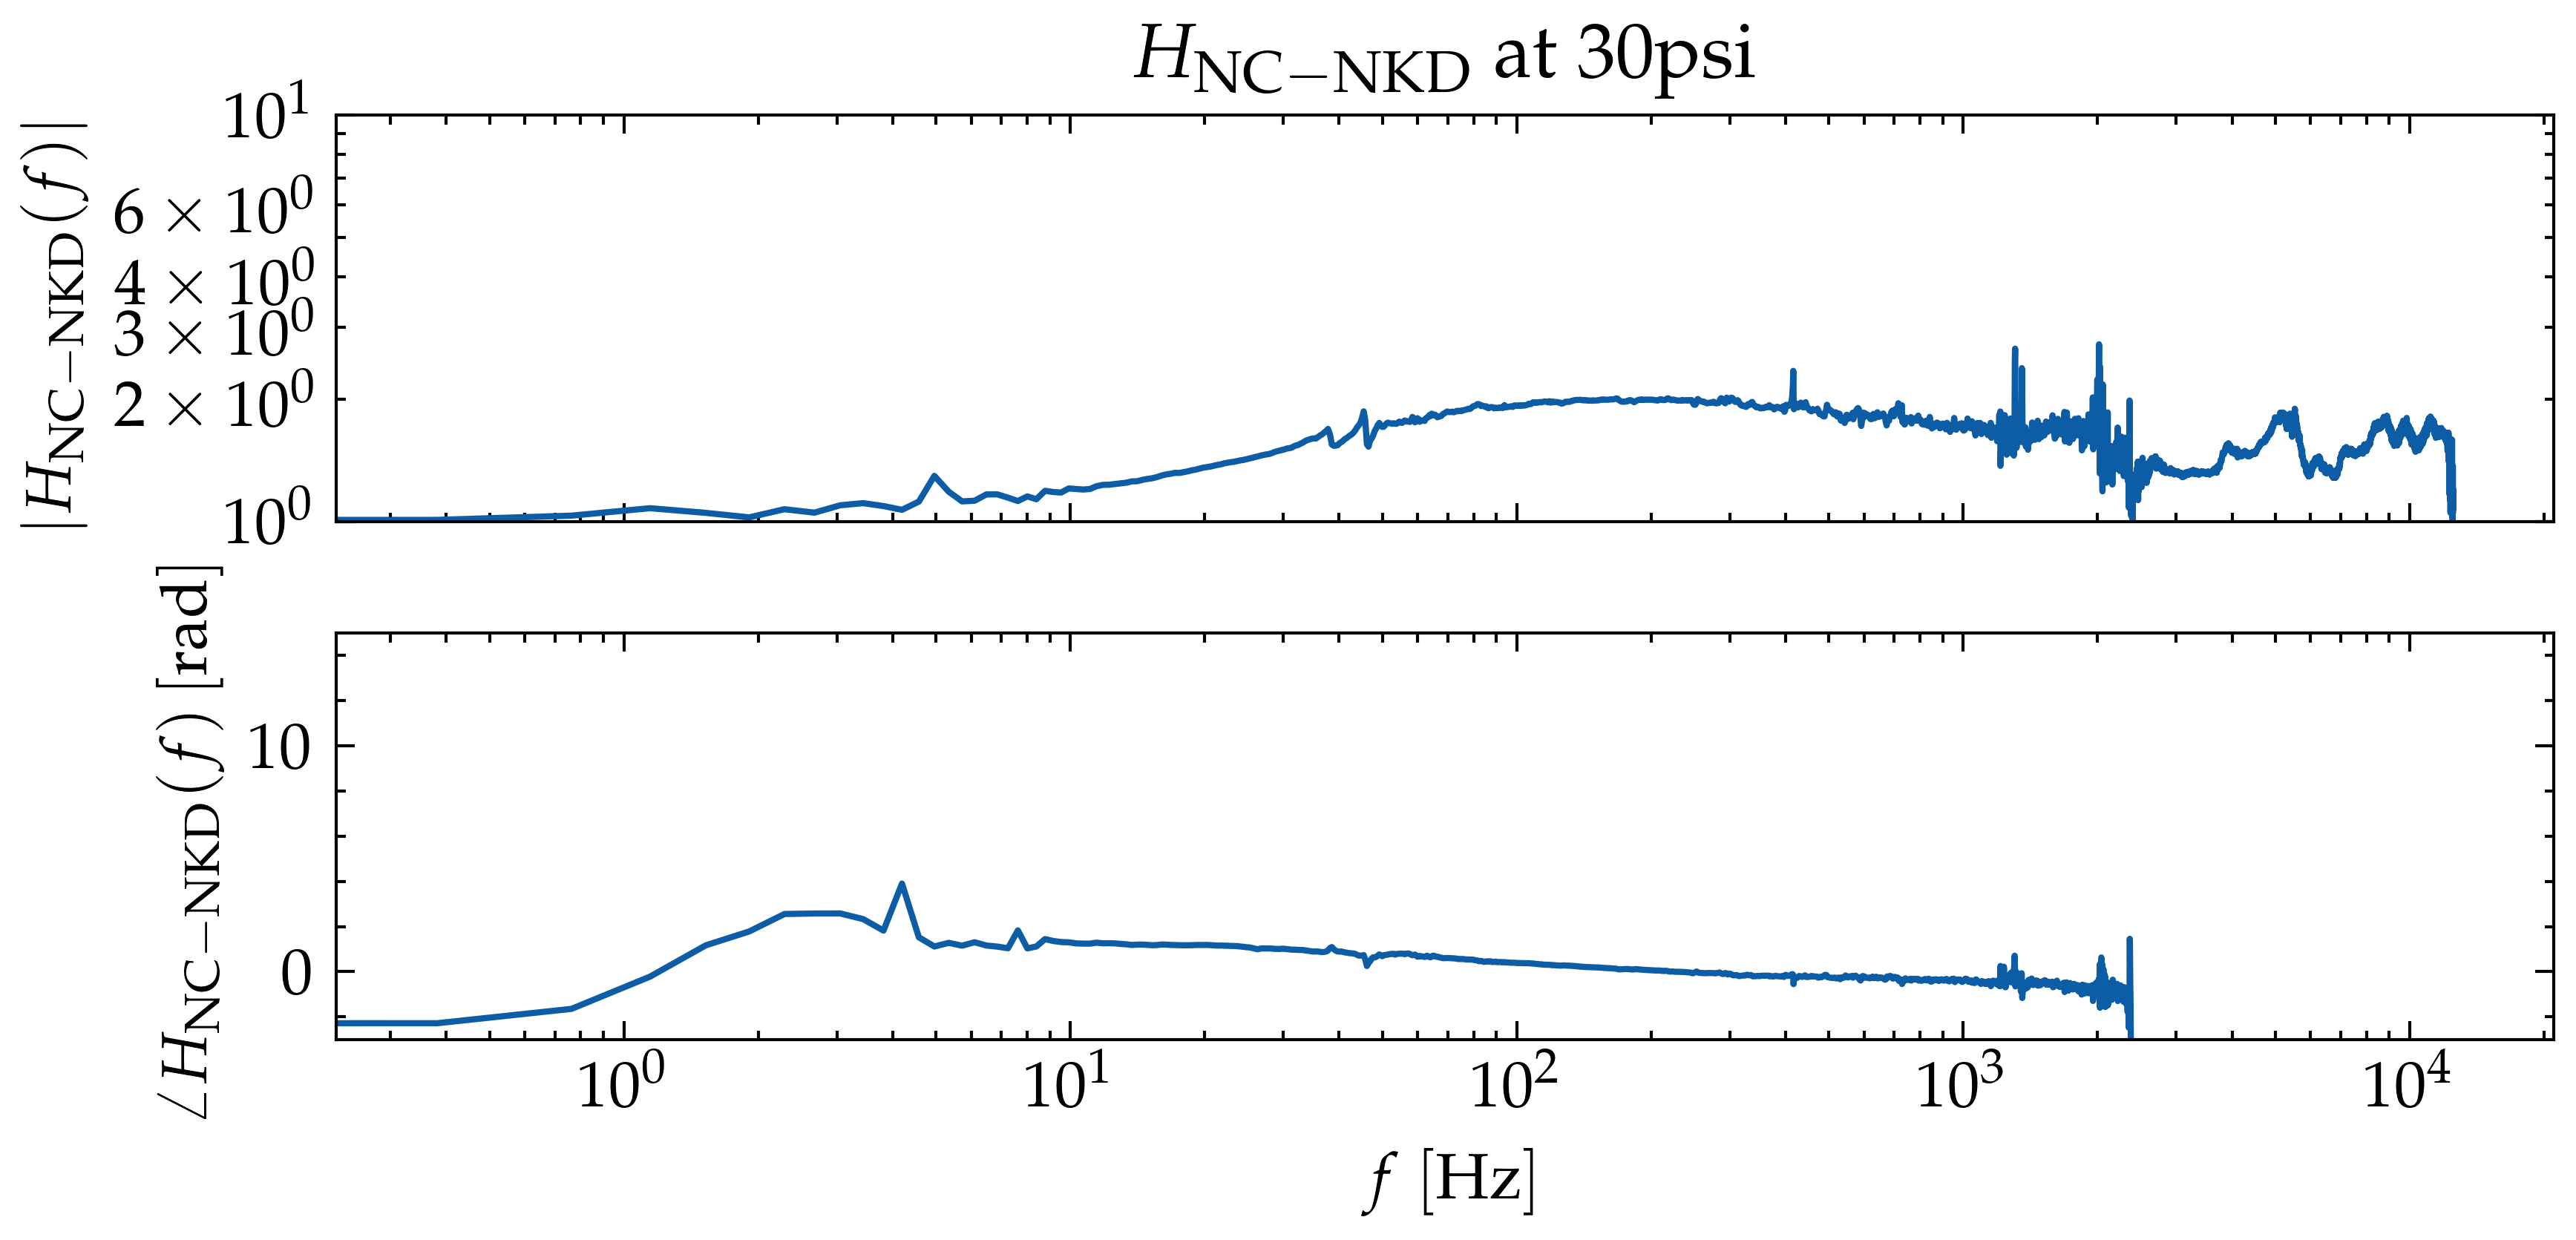
\includegraphics[width=0.8\linewidth]{NC-NKD/H_30psi.png}
            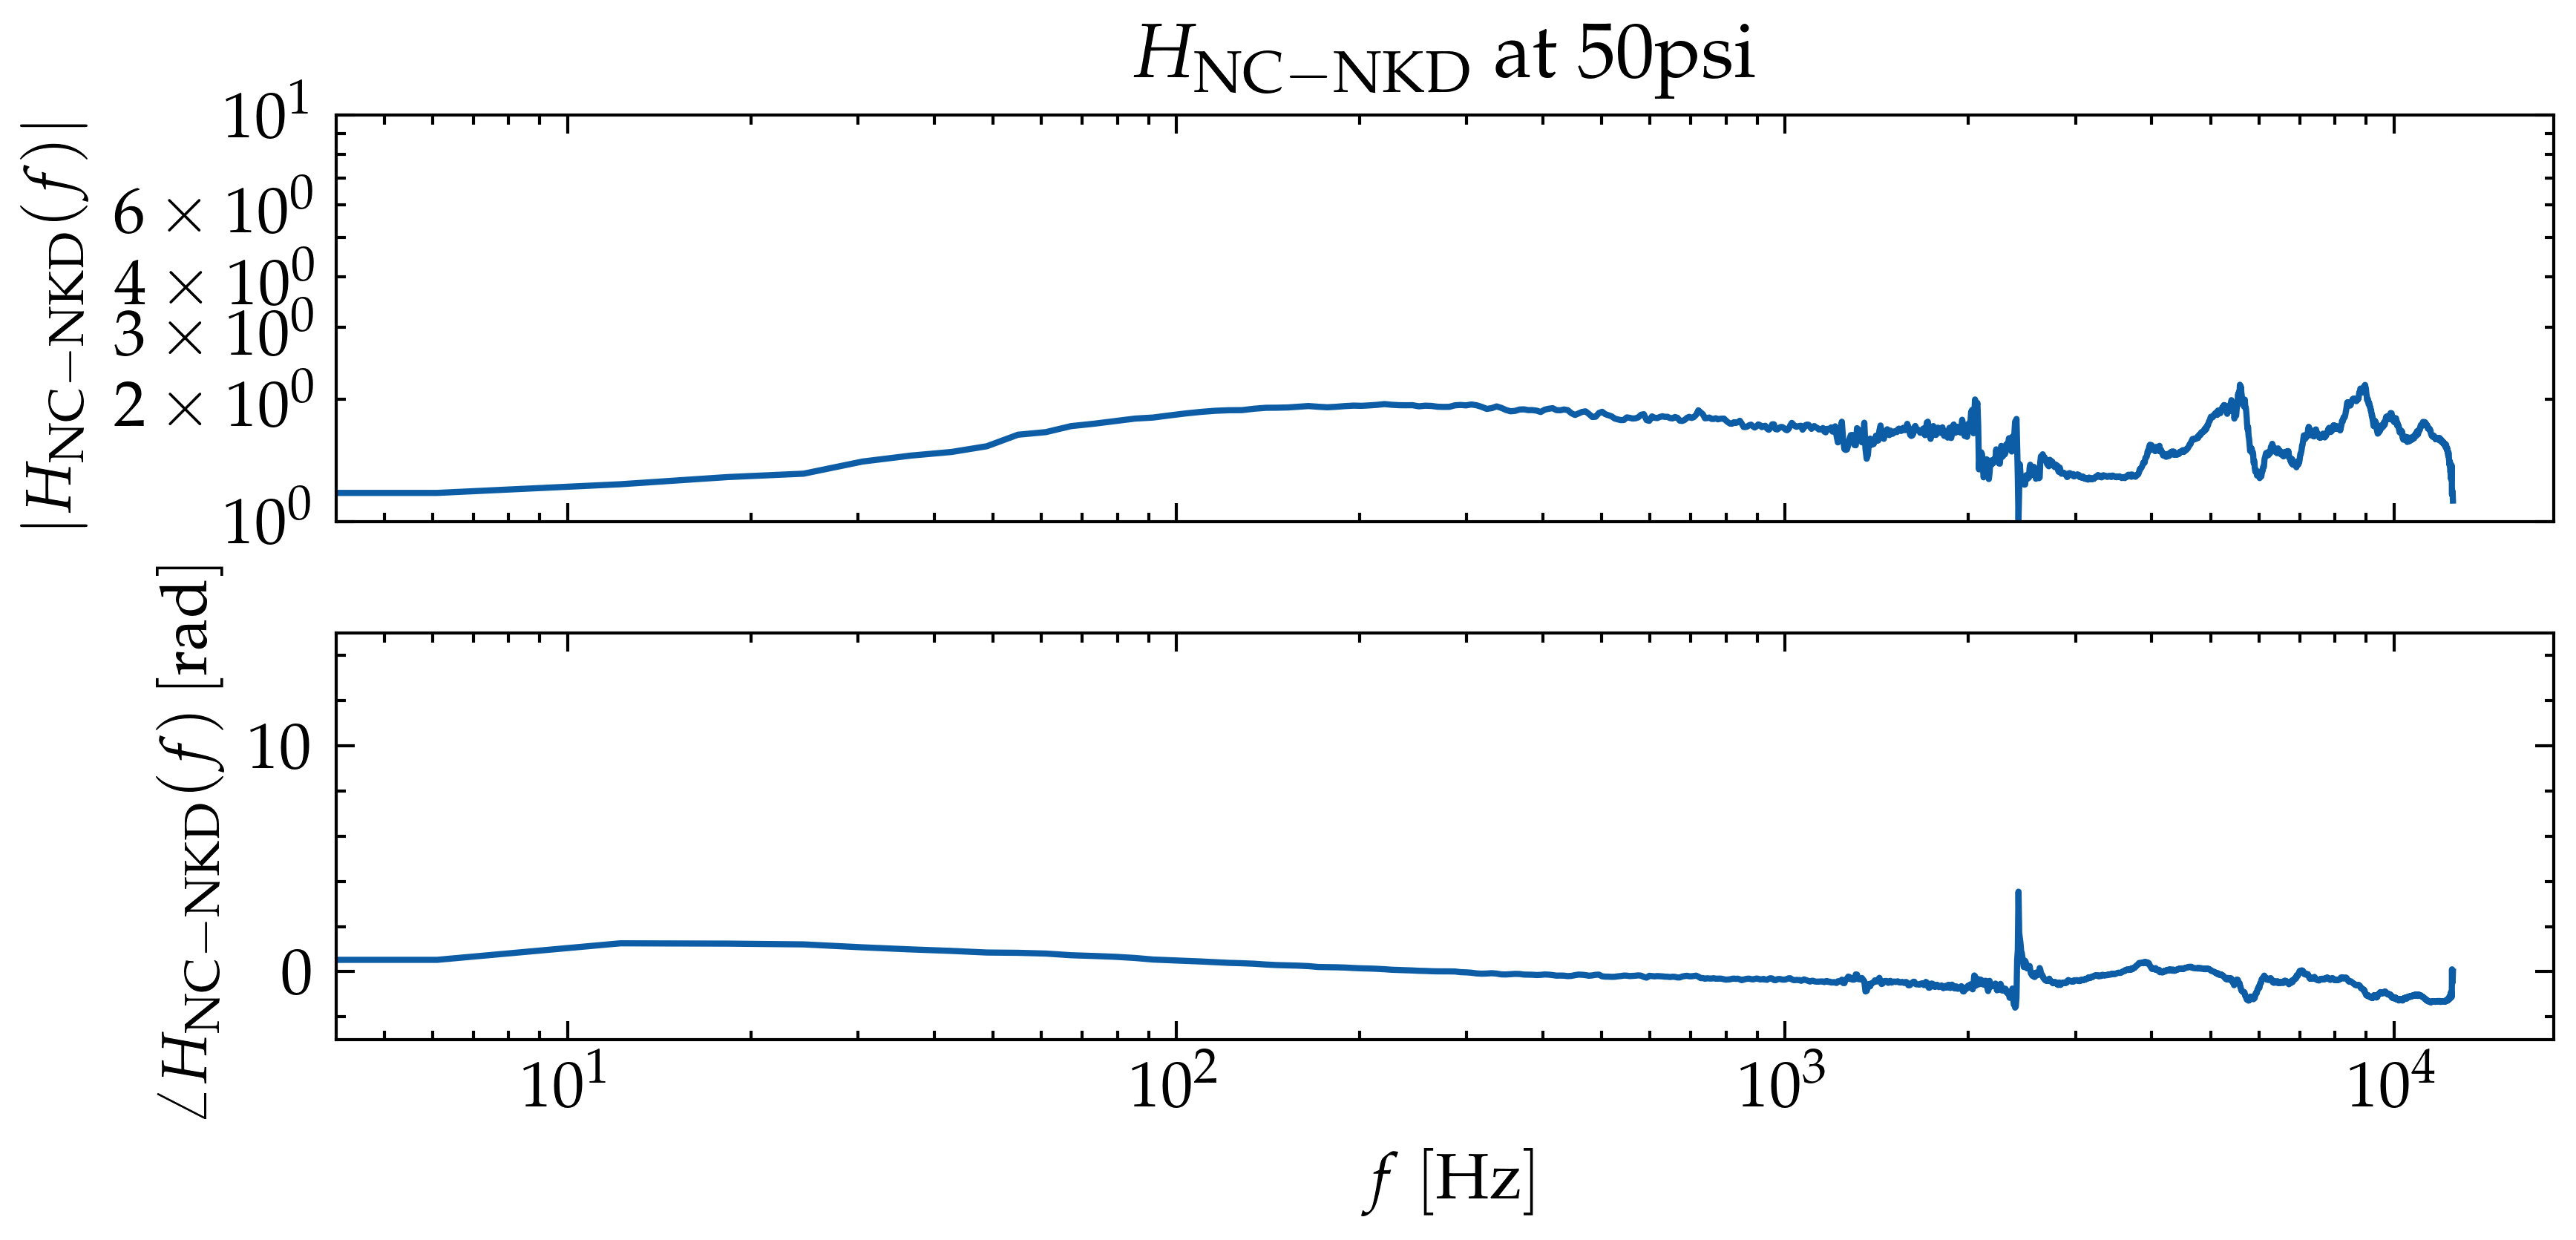
\includegraphics[width=0.8\linewidth]{NC-NKD/H_50psi.png}
            % 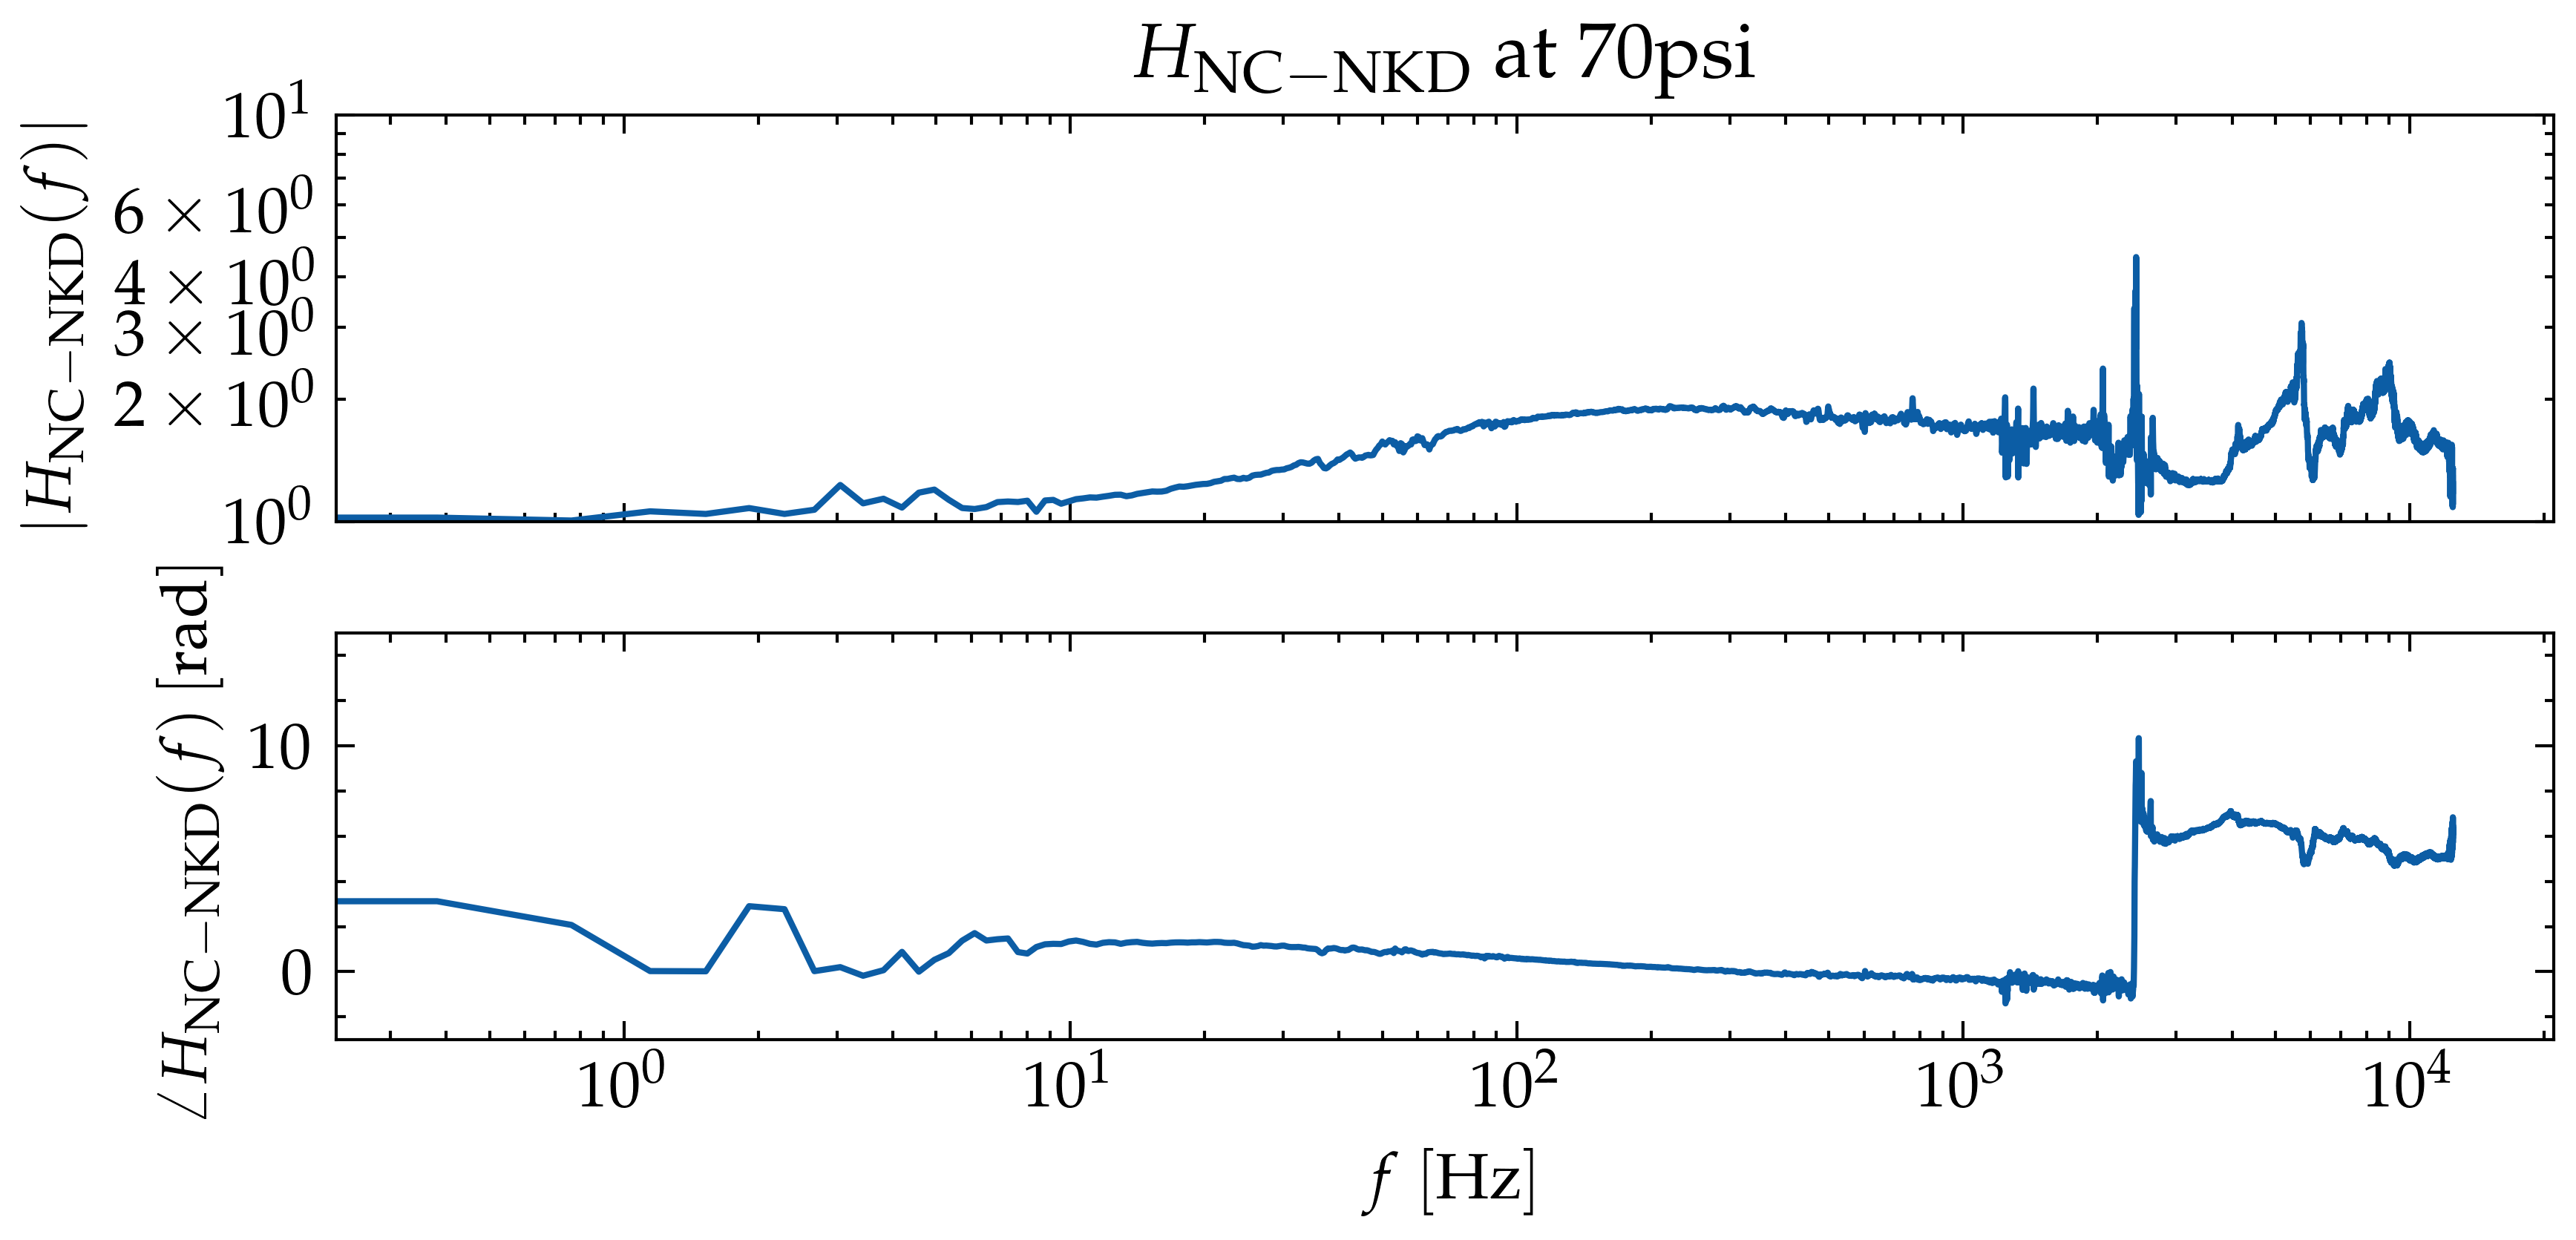
\includegraphics[width=0.8\linewidth]{NC-NKD/H_70psi.png}
            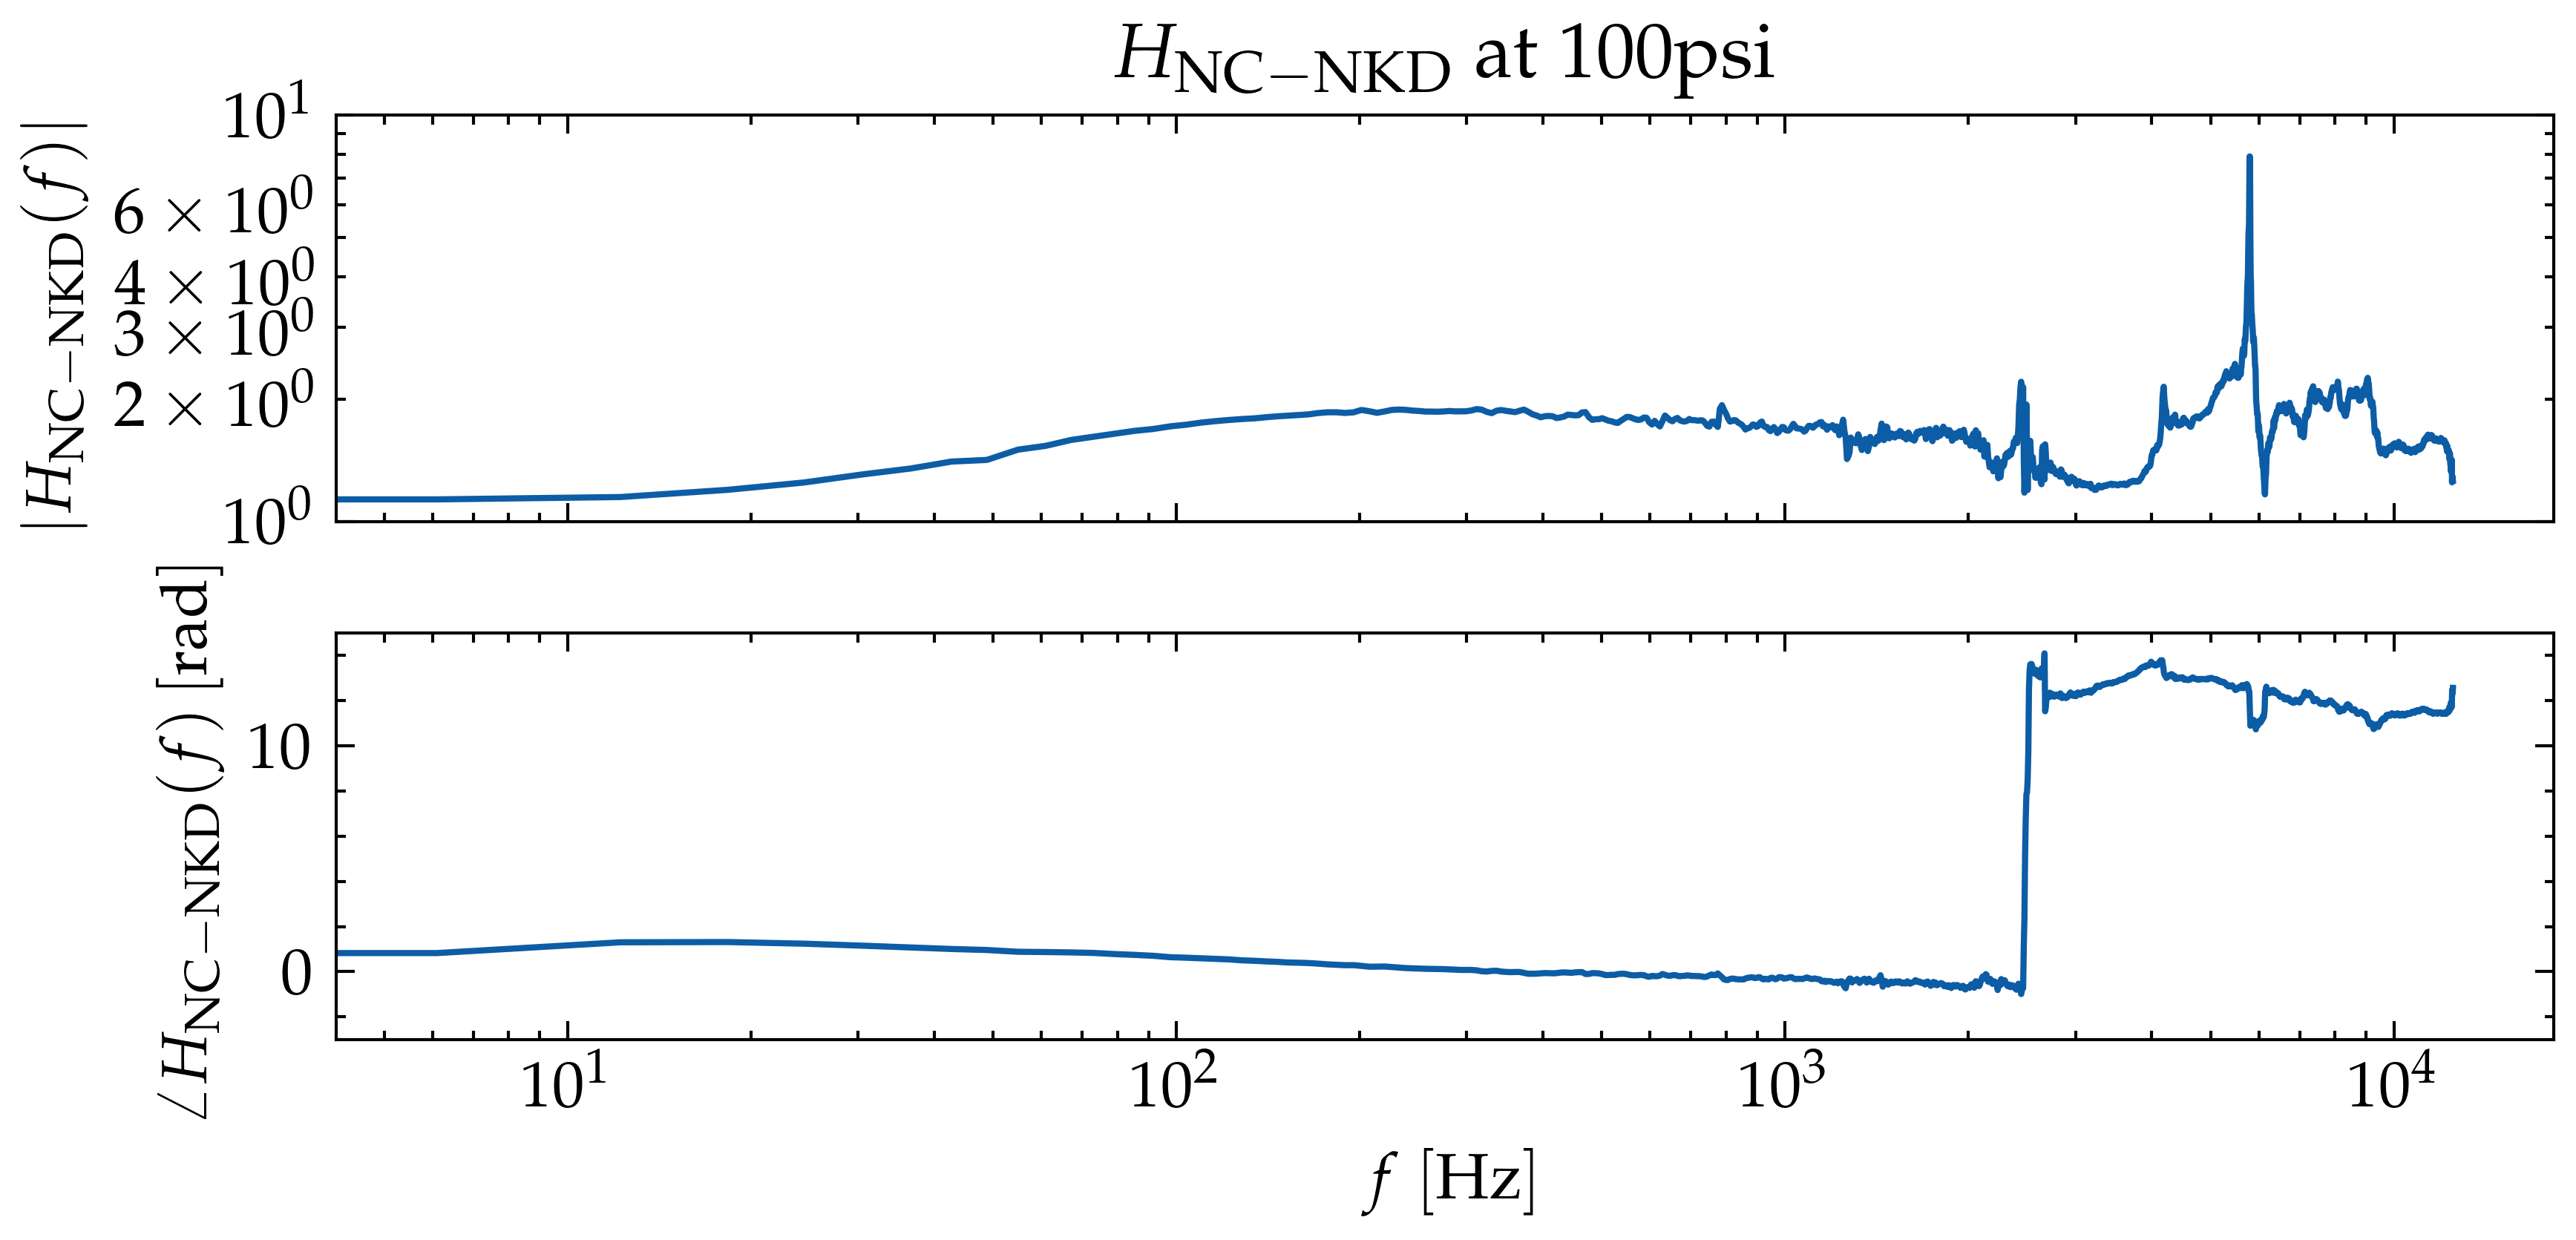
\includegraphics[width=0.8\linewidth]{NC-NKD/H_100psi.png}
    \end{columns}
\end{frame}

\begin{frame}
    \frametitle{Microphone calibration: Pinhole (PH)}
    \begin{columns}[c] % vertically centered
        \column{0.55\textwidth}
            \centering
            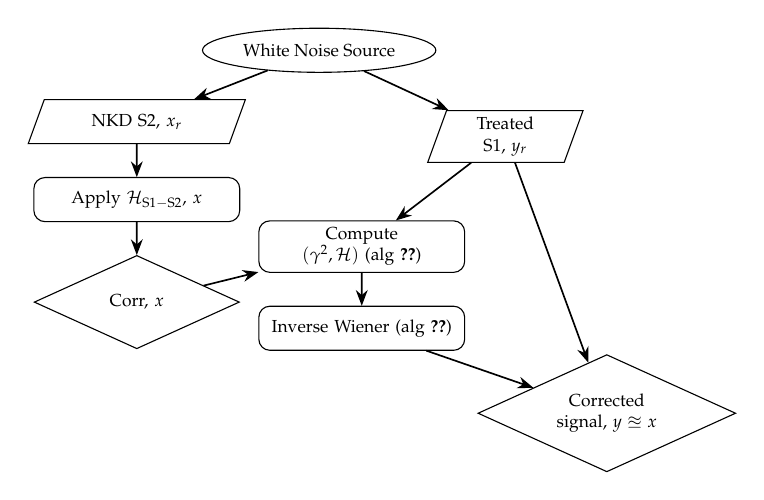
\begin{tikzpicture}[scale=0.7, transform shape,
                node distance=6mm and 18mm, every node/.style={font=\small}]
                \node (start) [terminator] {White Noise Source};

                % Two separate measurement boxes
                \node (refraw)   [meas, below left = 6mm and 14mm of start, anchor=north east]
                    {NKD S2, $x_r$};

                \node (S1S2) [proc, below=of refraw]
                    {Apply $\mathcal{H}_{\mathrm{S1-S2}}$, $x$};

                \node (ref) [decision, below=of S1S2]
                    {Corr, $x$};

                \node (treat) [meas, below right = 8mm and 14mm of start, anchor=north west]
                    {Treated S1, $y_r$};

                \node (H)  [proc, below left = 28mm and -4mm of start, anchor=north west]
                    {Compute $(\gamma^2,\mathcal{H})$ (alg~\ref{alg:H})};


                \node (wien)  [proc, below=of H]
                    {Inverse Wiener (alg~\ref{alg:inv})};

                \node (corr)  [decision, below right = 6mm and 14mm of wien]
                    {Corrected signal, $y \approxeq x$};

                \draw [line] (start) -- (refraw);
                \draw [line] (start) -- (treat);
                \draw [line] (refraw) -- (S1S2);
                \draw [line] (S1S2) -- (ref);
                \draw [line] (ref) -- (H);
                \draw [line] (treat) -- (H);
                \draw [line] (H) -- (wien);
                \draw [line] (wien) -- (corr);
                \draw [line] (treat) -- (corr);

            \end{tikzpicture}
        \column{0.4\textwidth}
            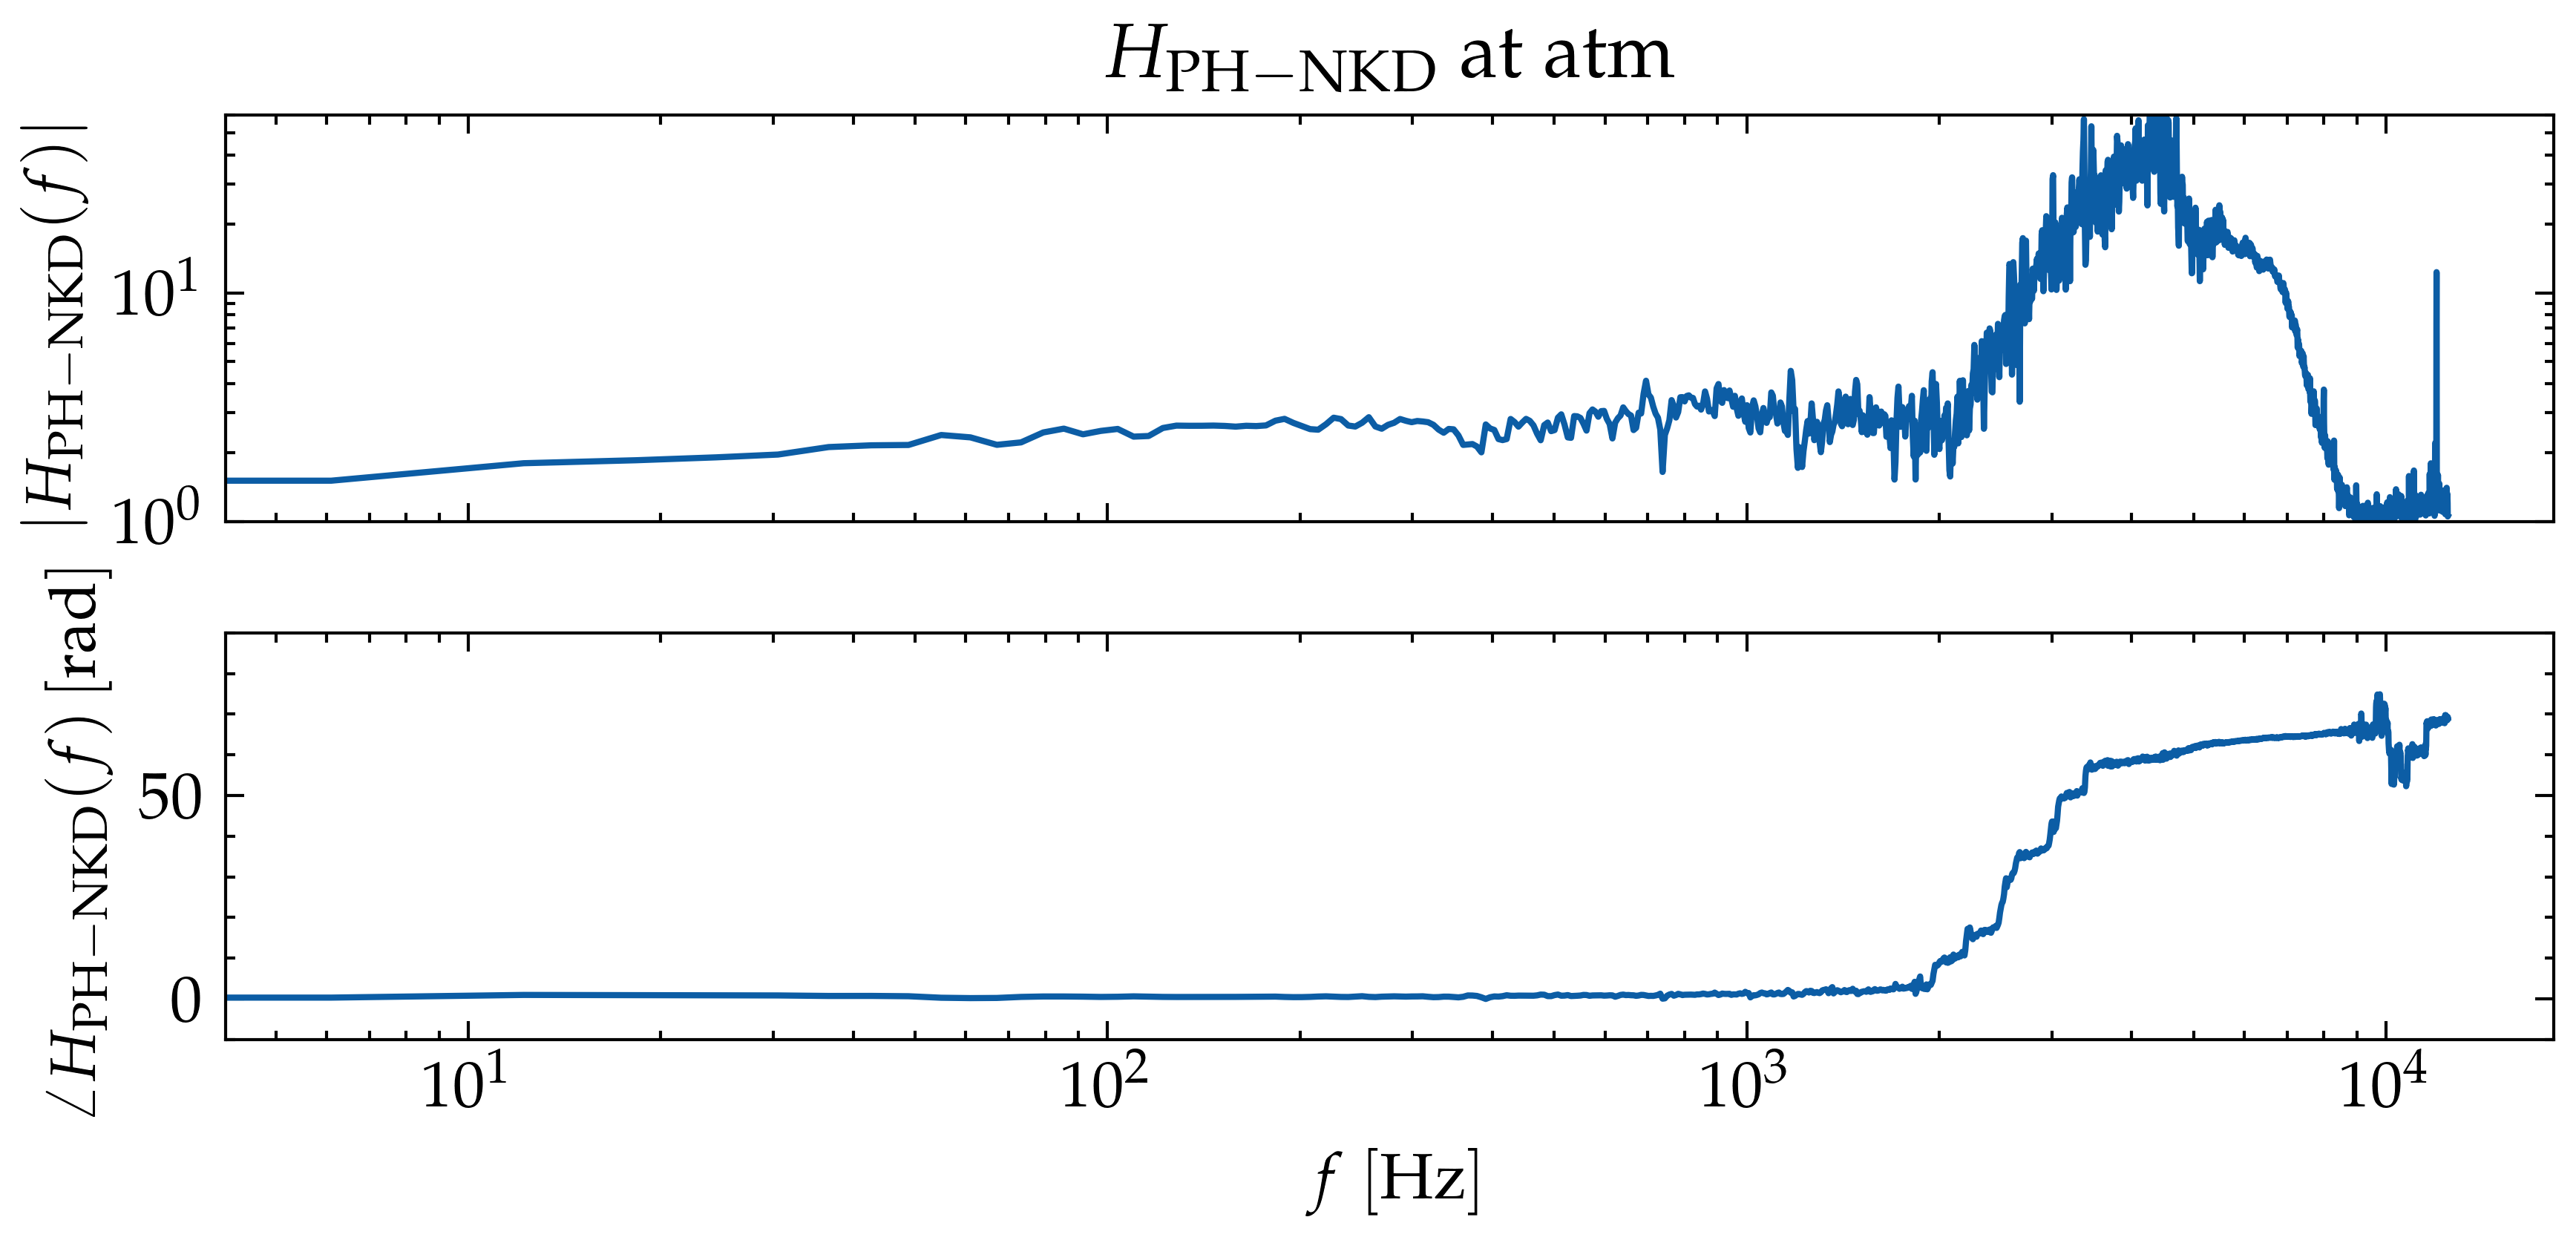
\includegraphics[width=0.8\linewidth]{PH-NKD/H_atm.png}
            % 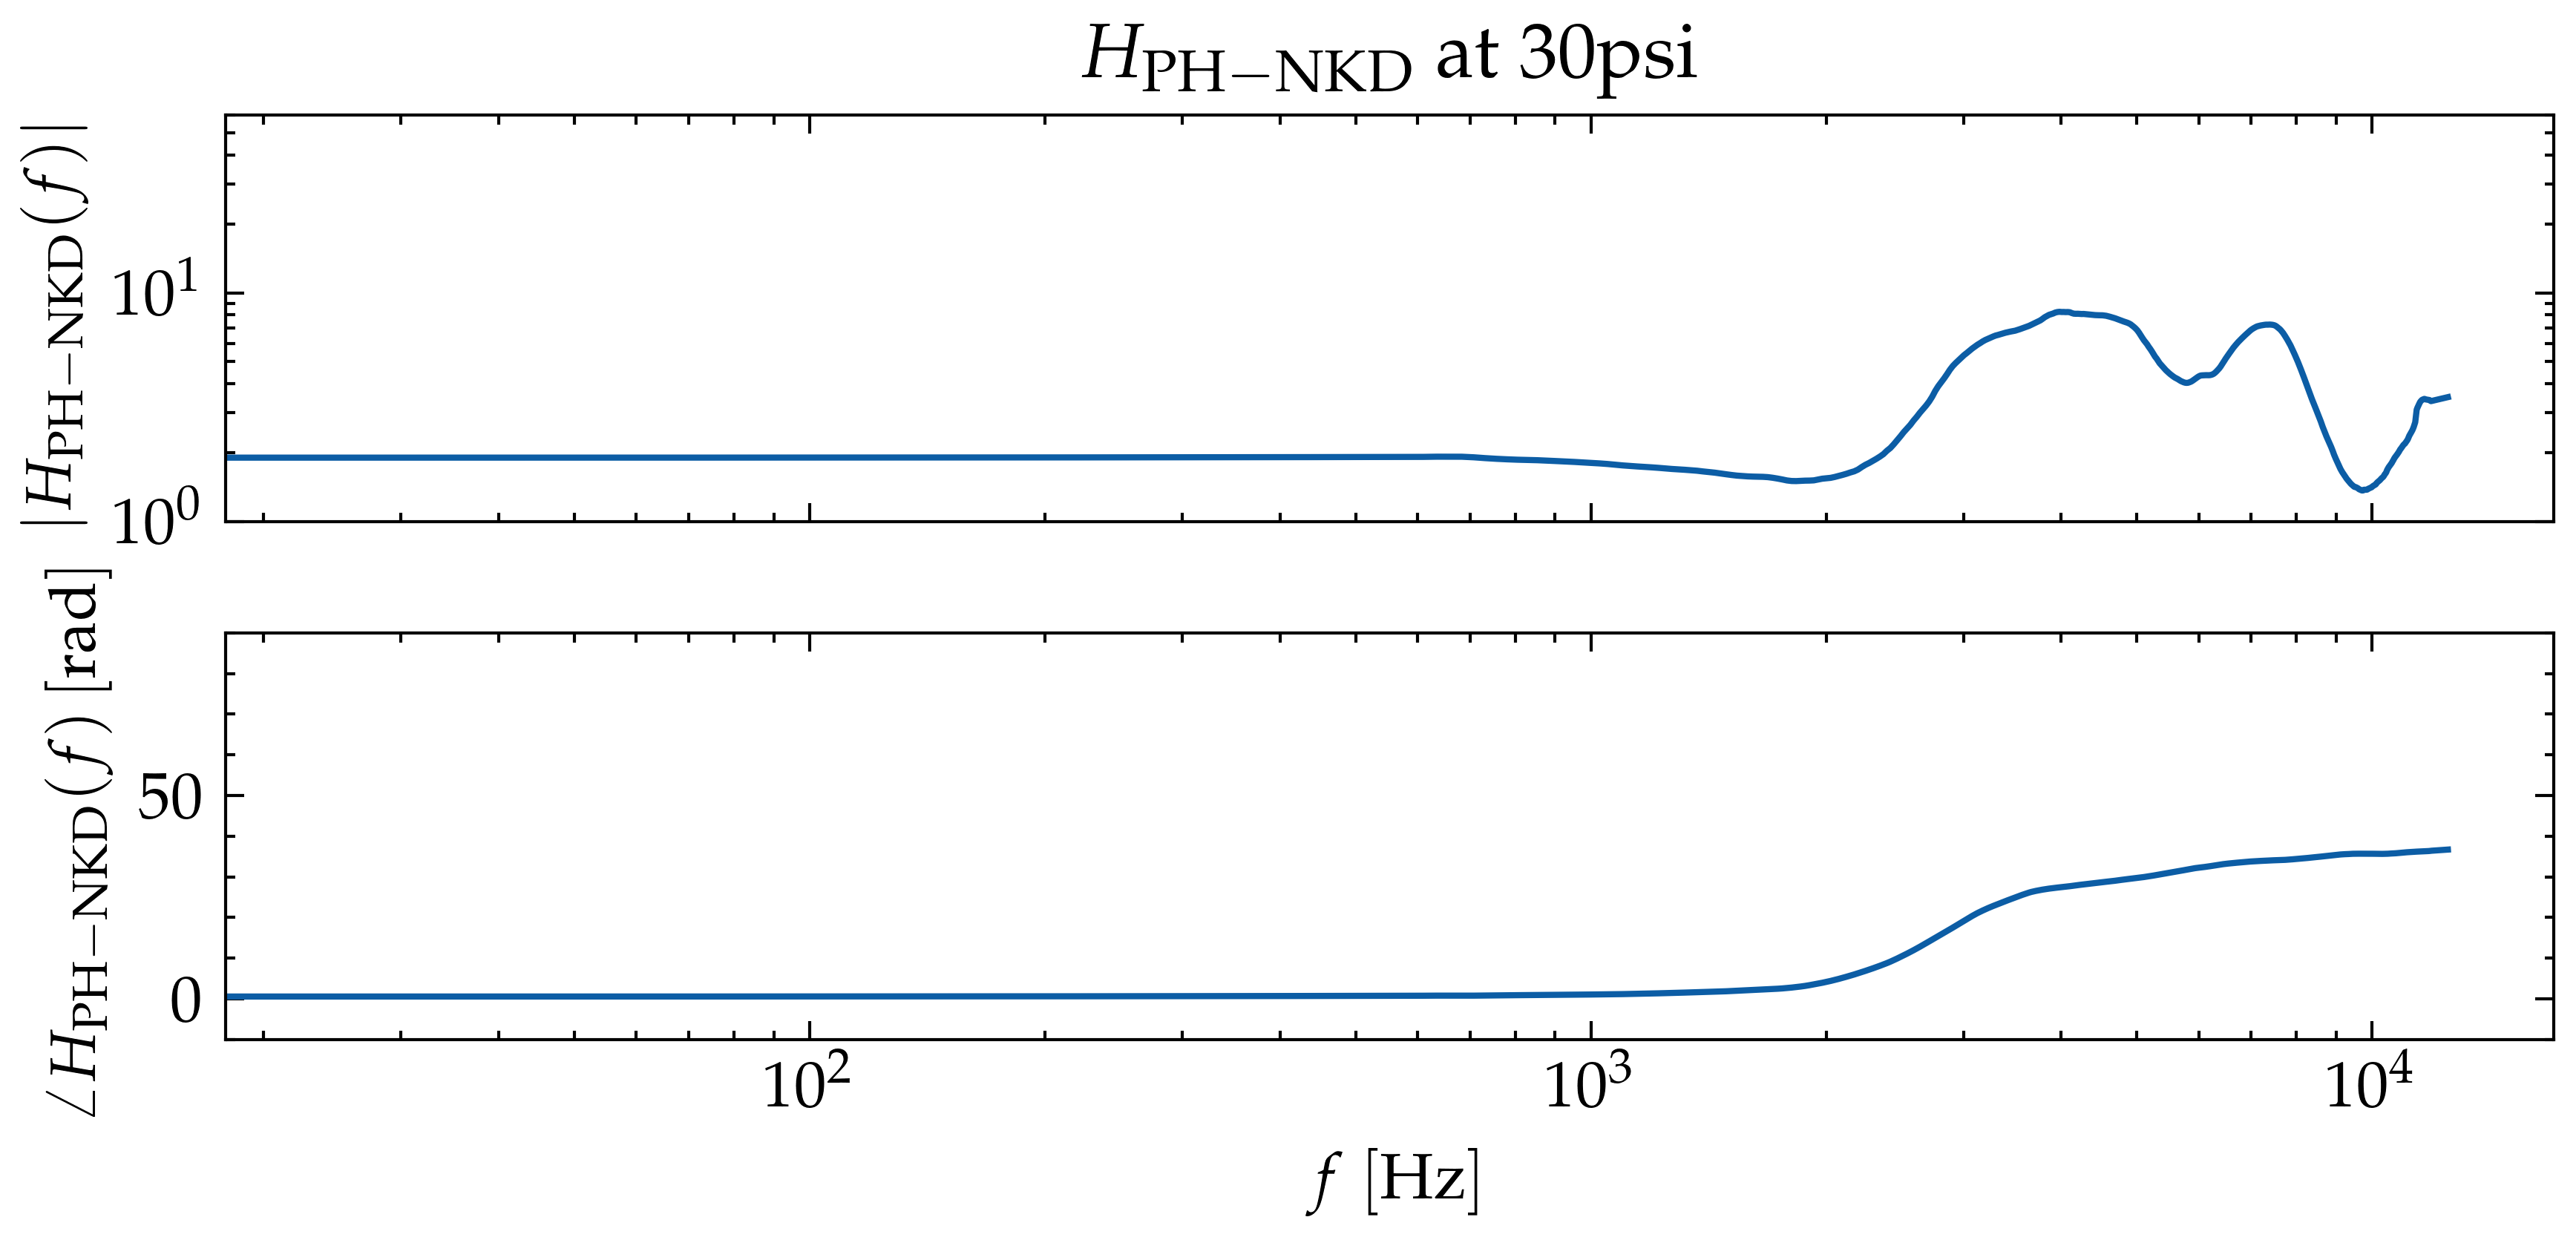
\includegraphics[width=0.8\linewidth]{PH-NKD/H_30psi.png}
            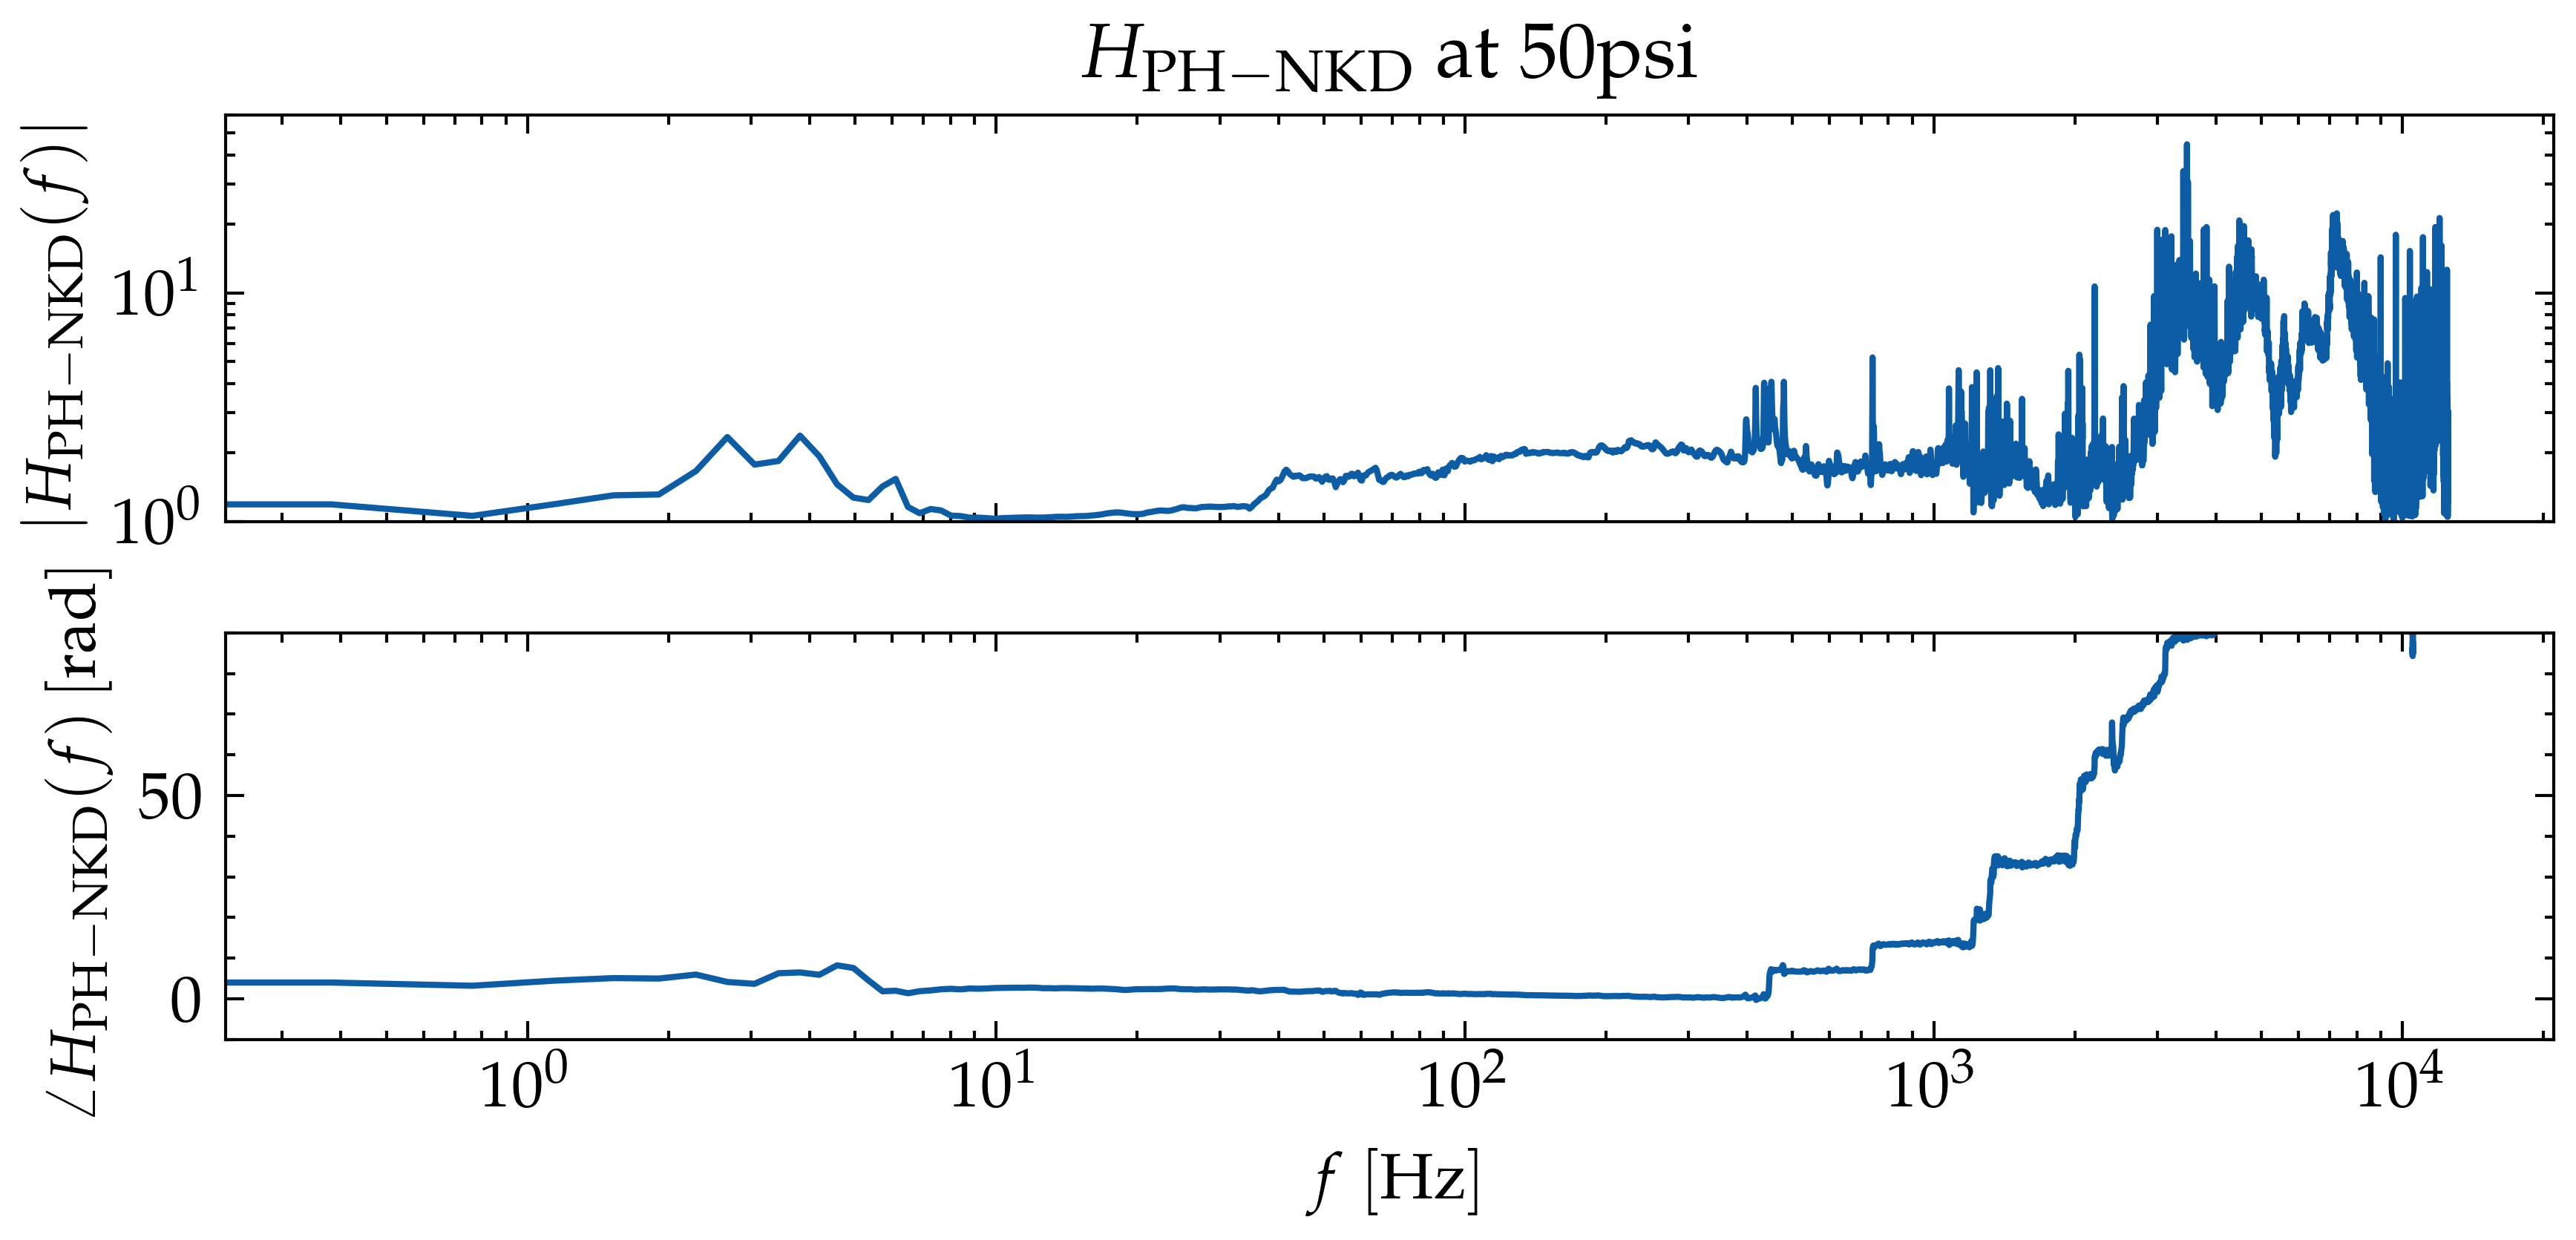
\includegraphics[width=0.8\linewidth]{PH-NKD/H_50psi.png}
            % 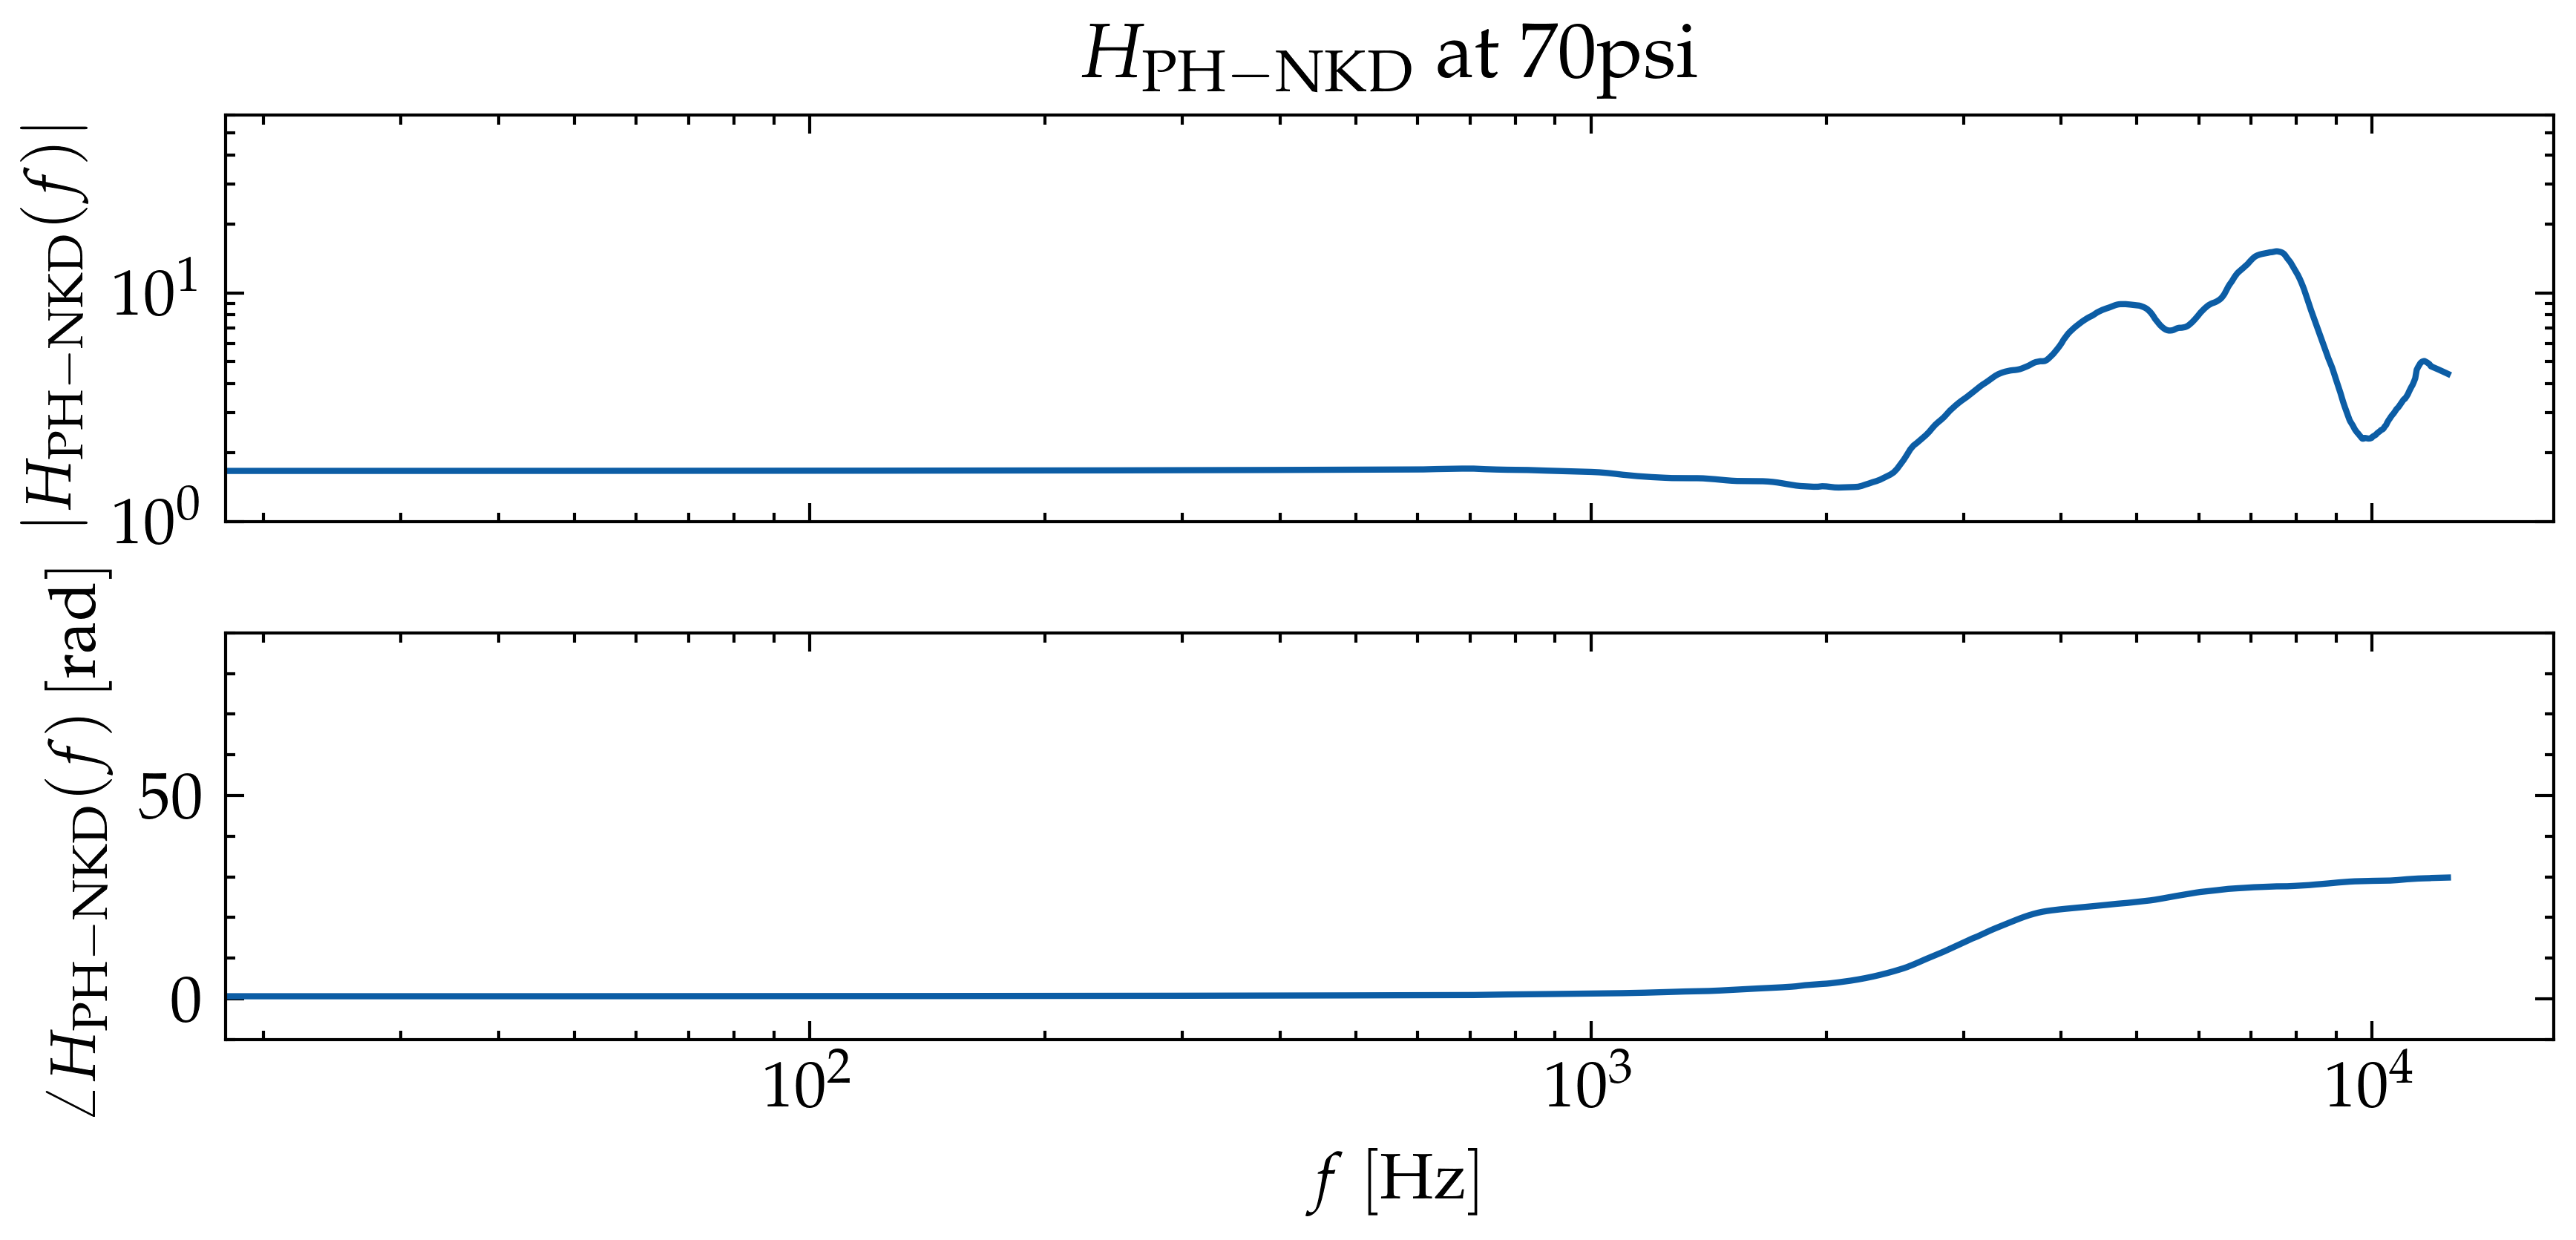
\includegraphics[width=0.8\linewidth]{PH-NKD/H_70psi.png}
            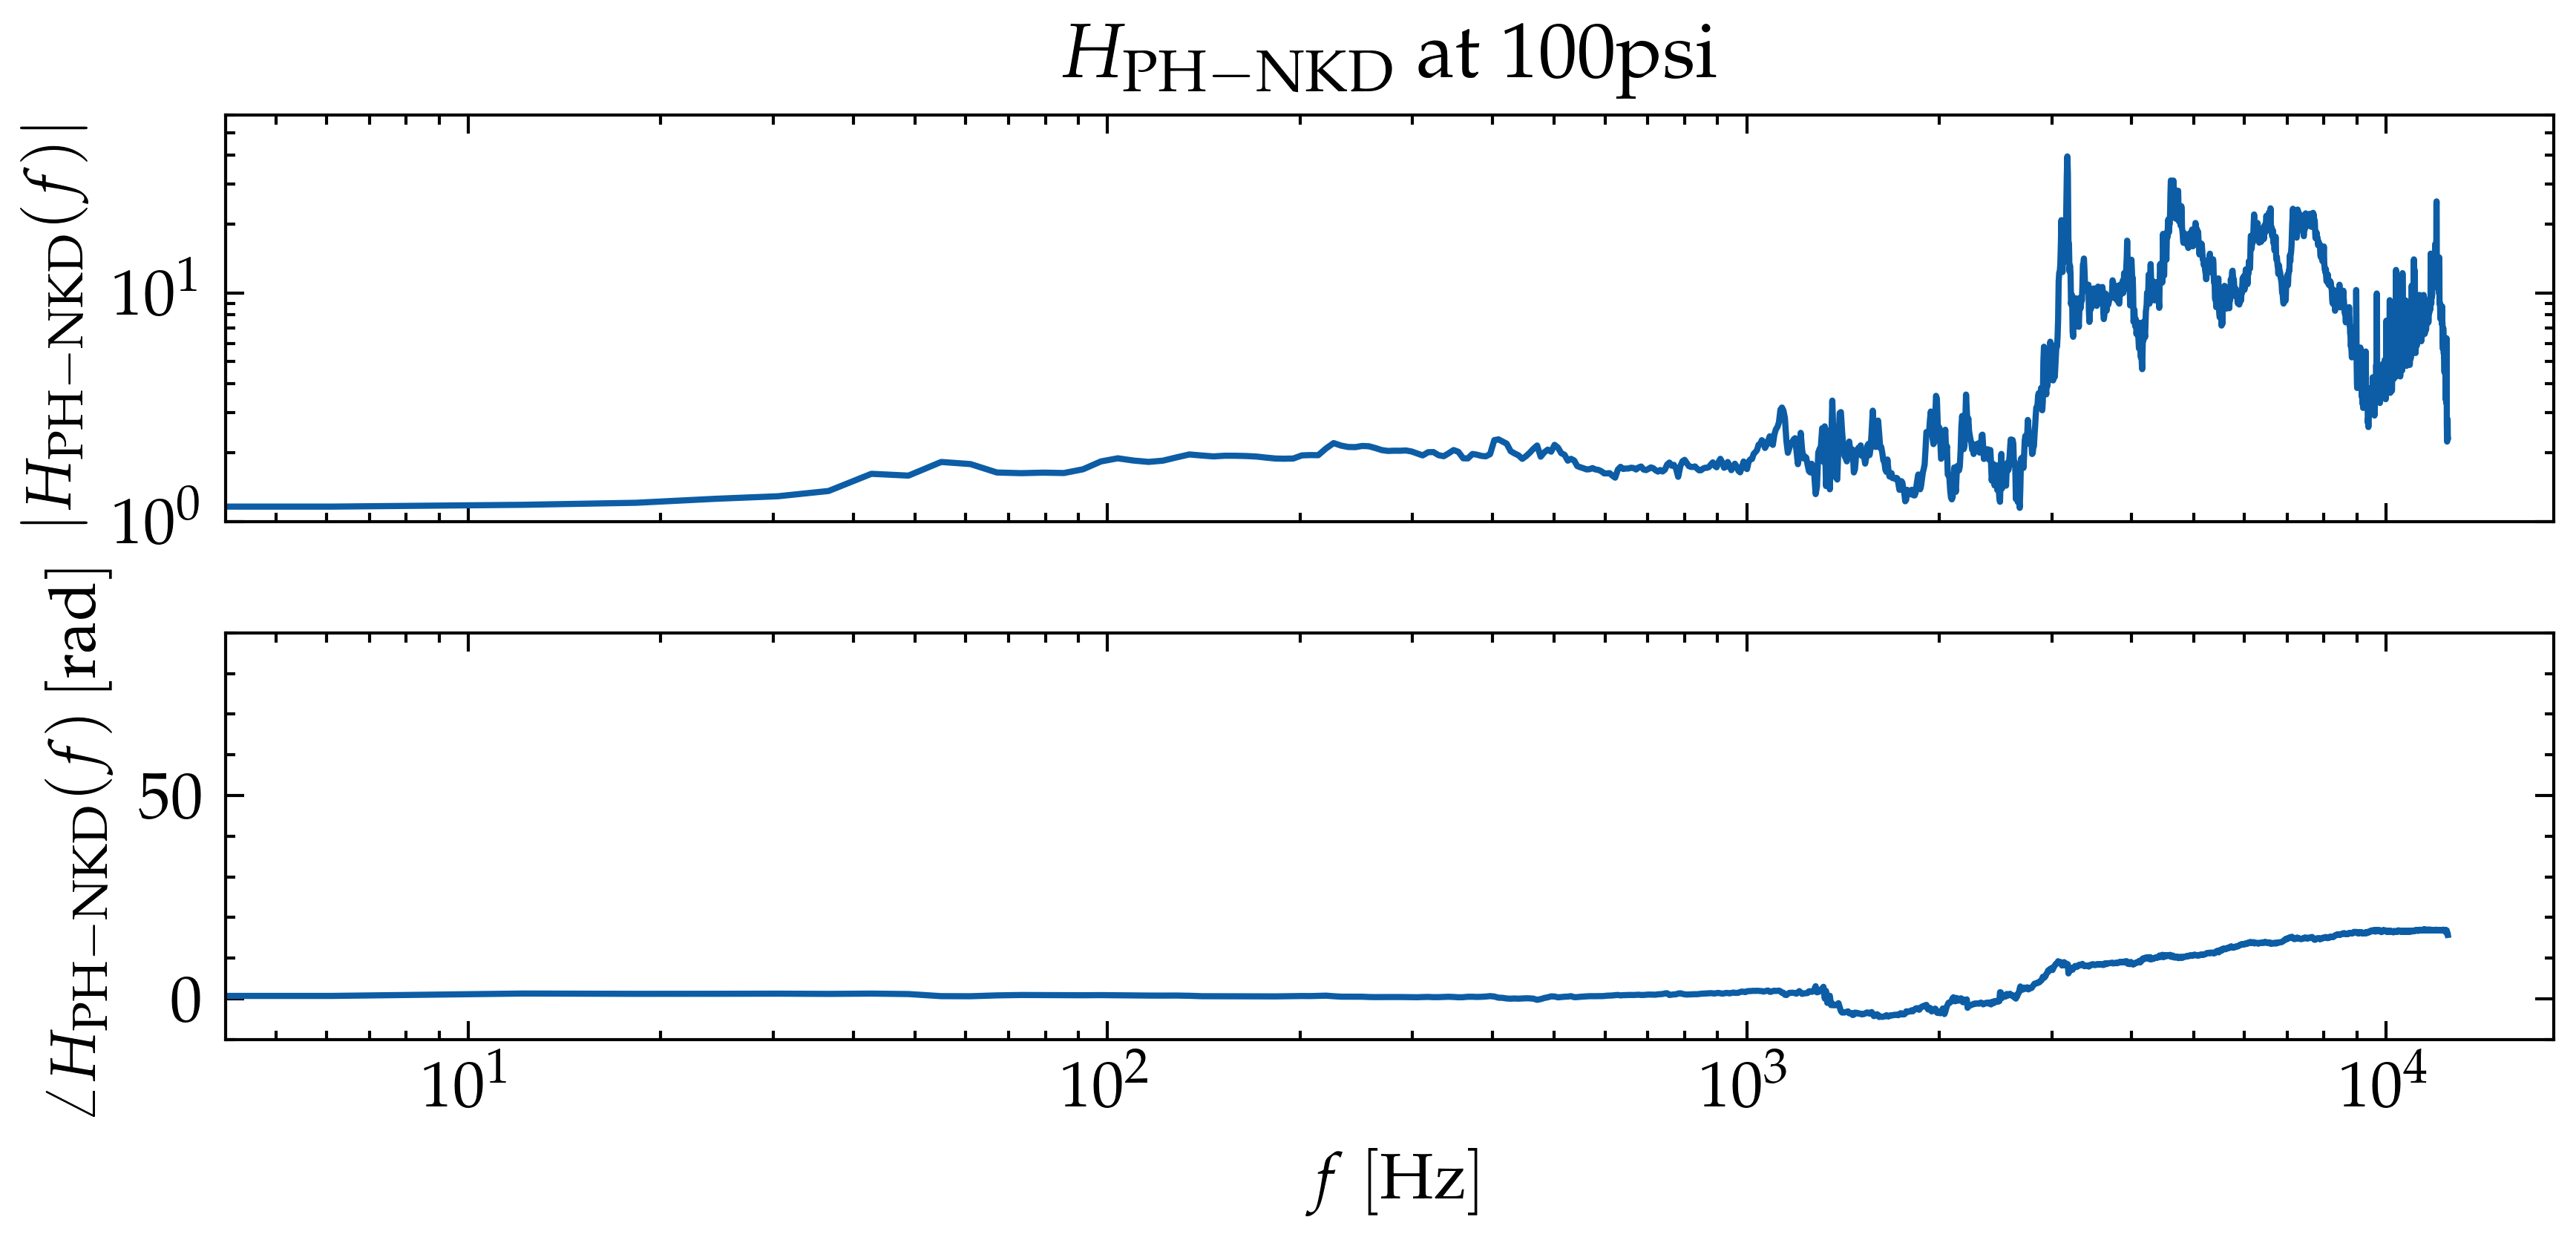
\includegraphics[width=0.8\linewidth]{PH-NKD/H_100psi.png}
    \end{columns}
\end{frame}

\begin{frame}
    \frametitle{Corrected signals}
    \begin{columns}[c]
        \column{0.3\textwidth}
        \centering
            Corrected NC trace
            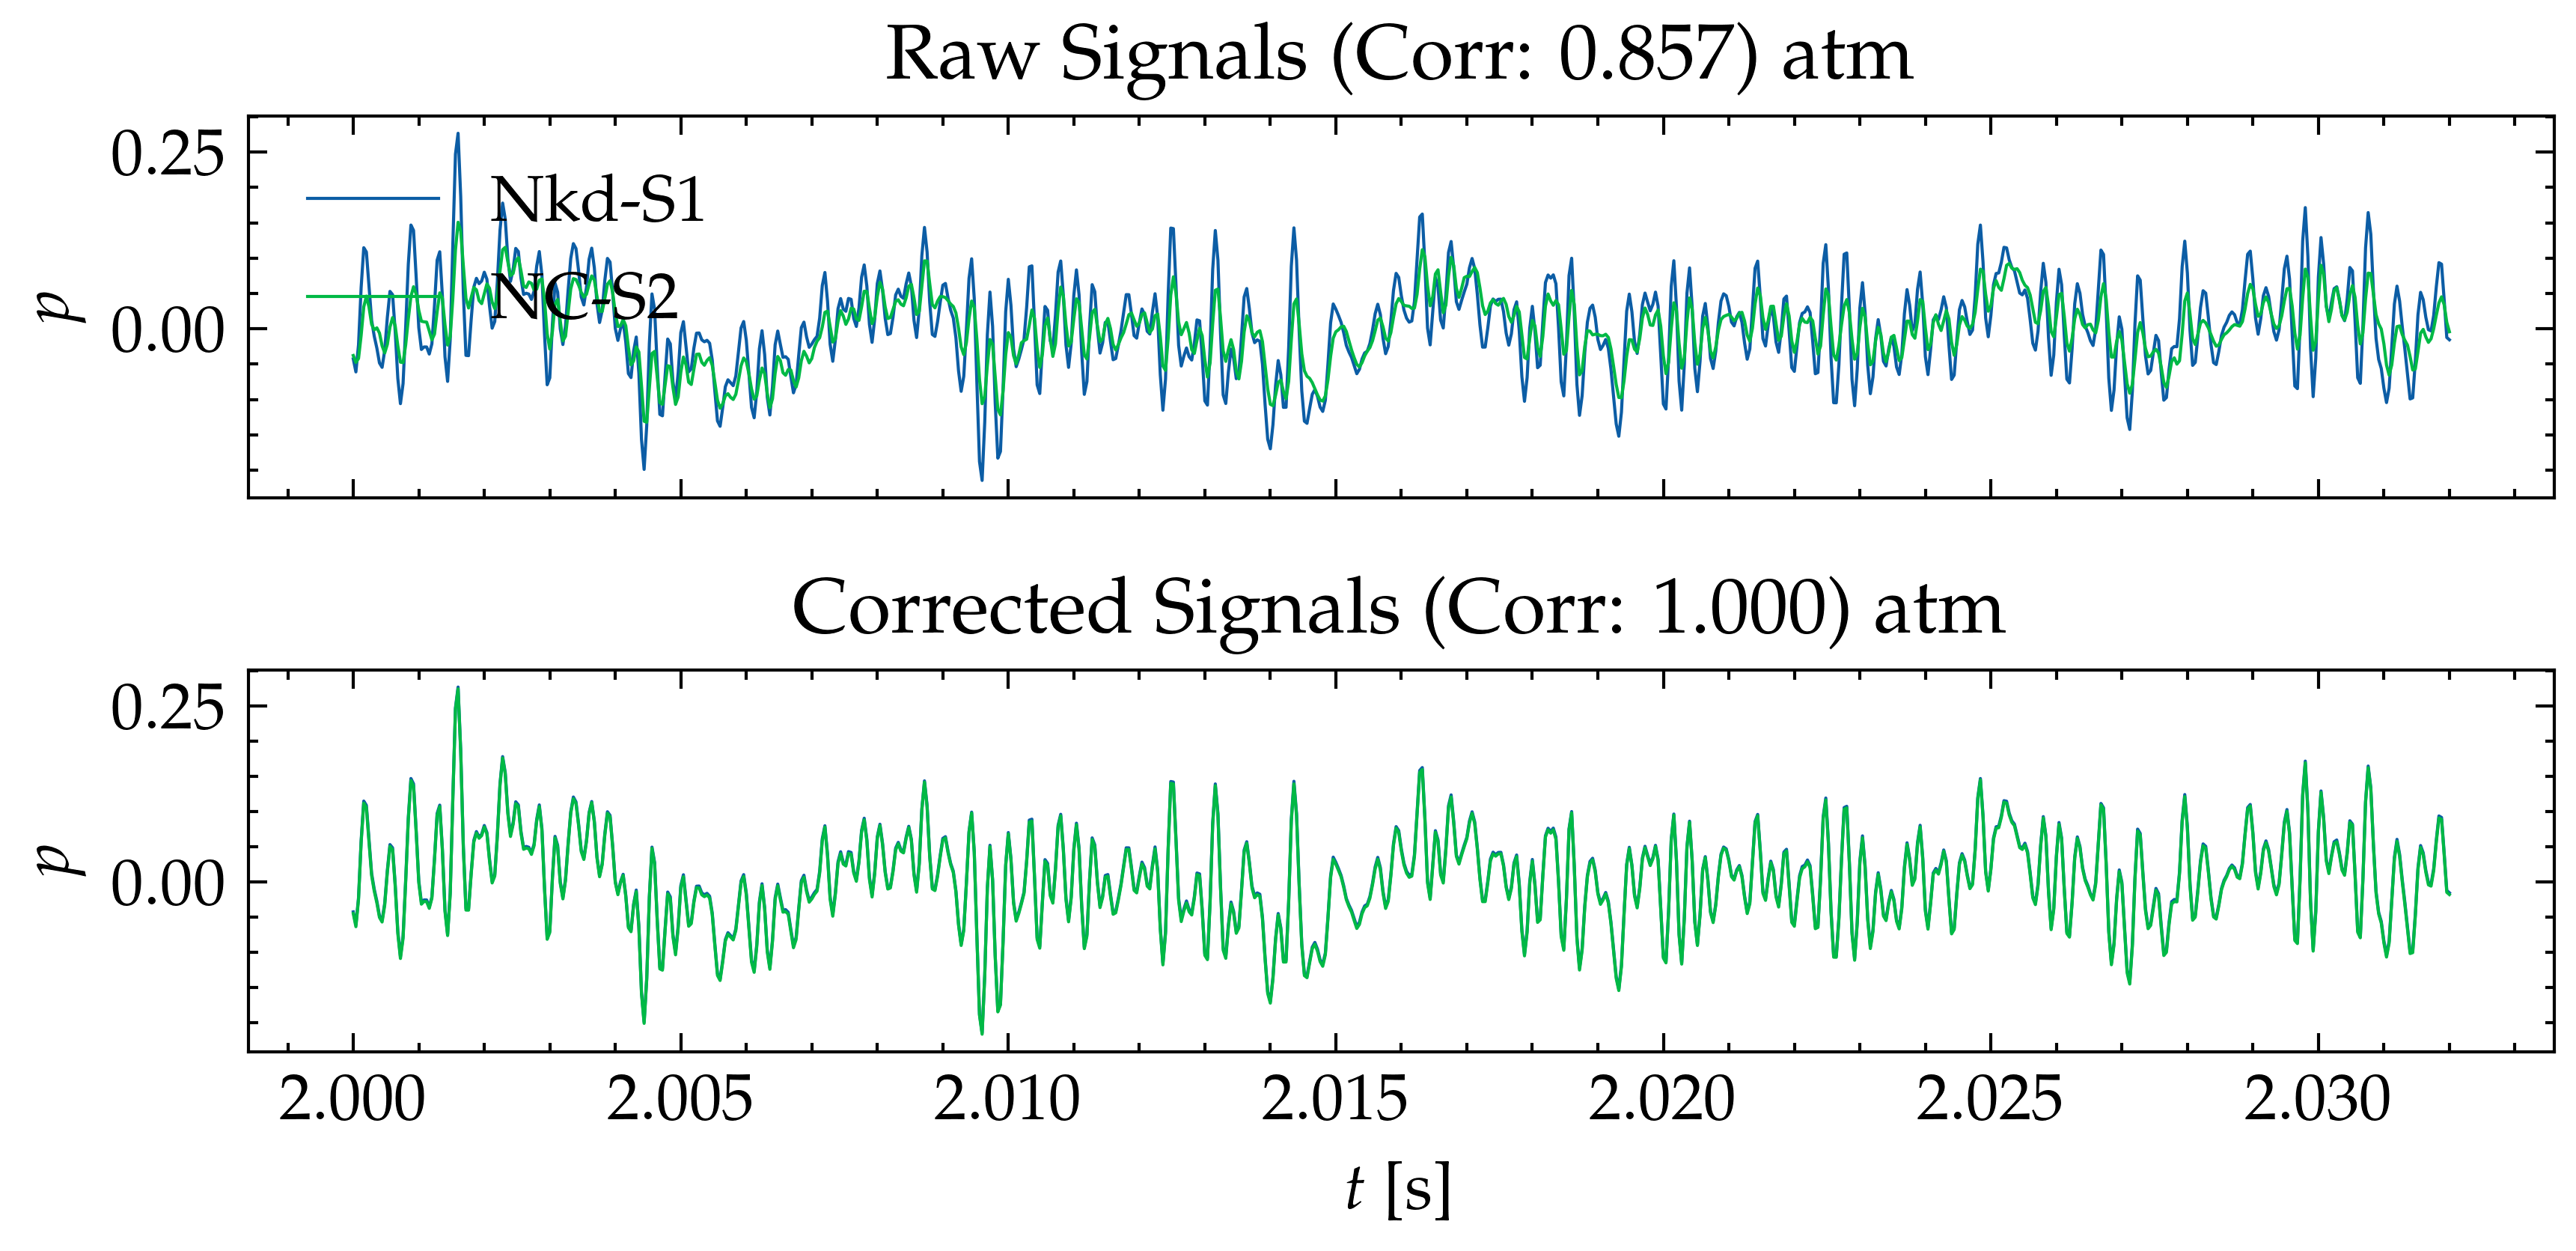
\includegraphics[width=\linewidth]{NC-NKD/y_atm.png}
            % 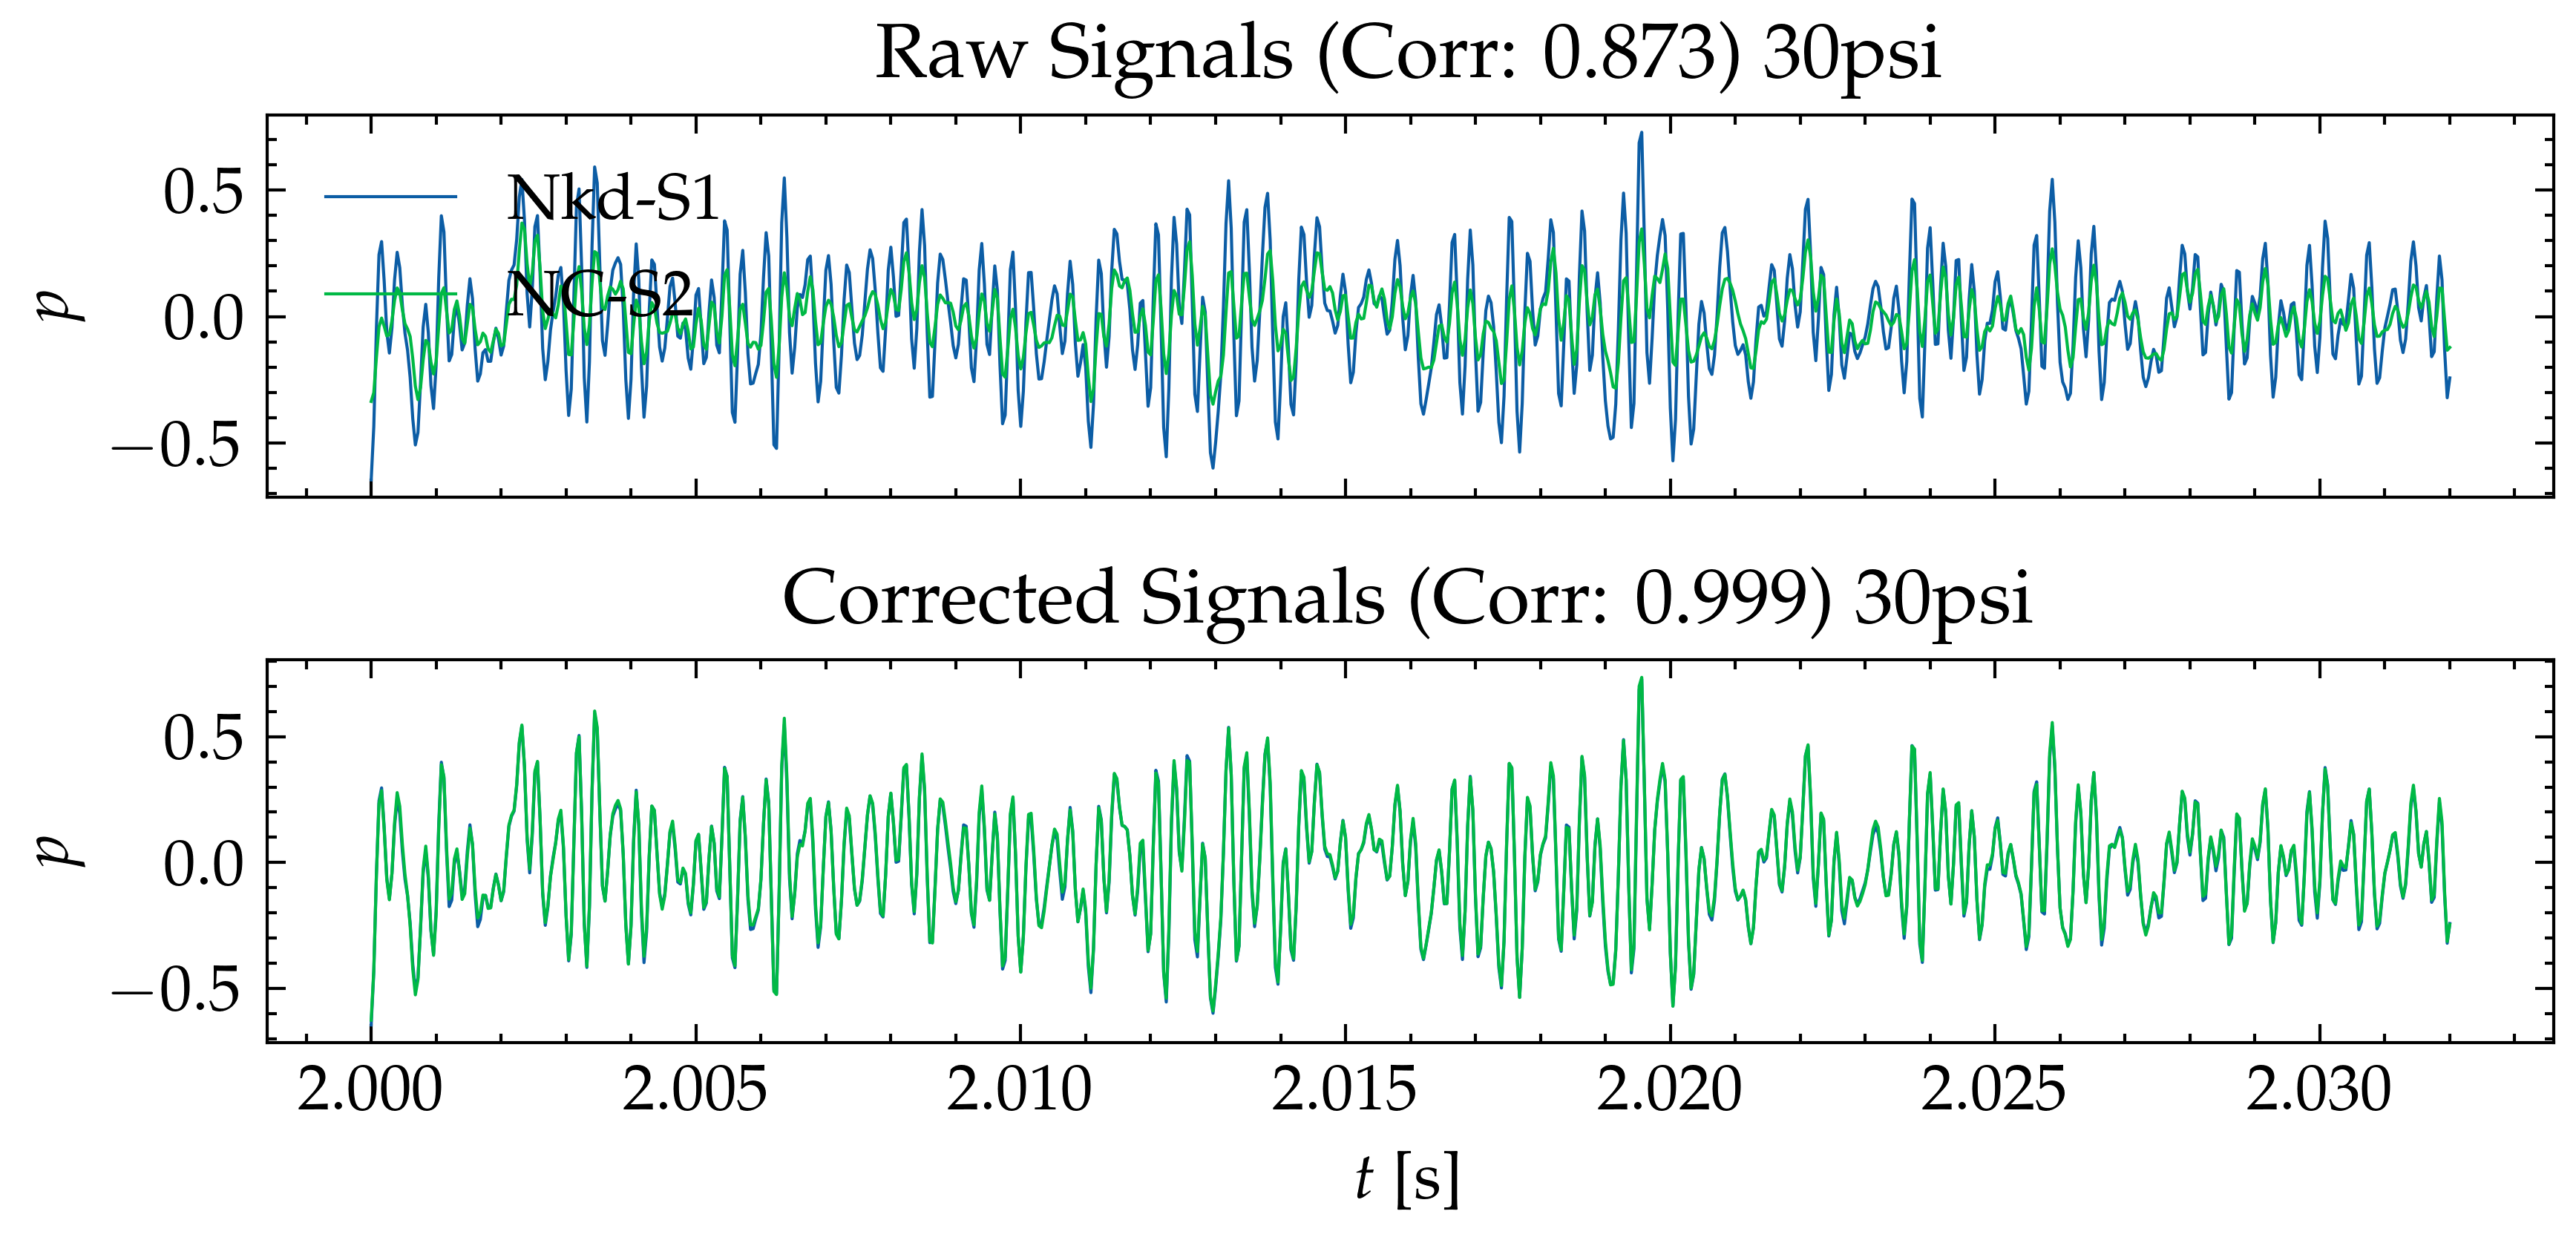
\includegraphics[width=\linewidth]{NC-NKD/y_30psi.png}
            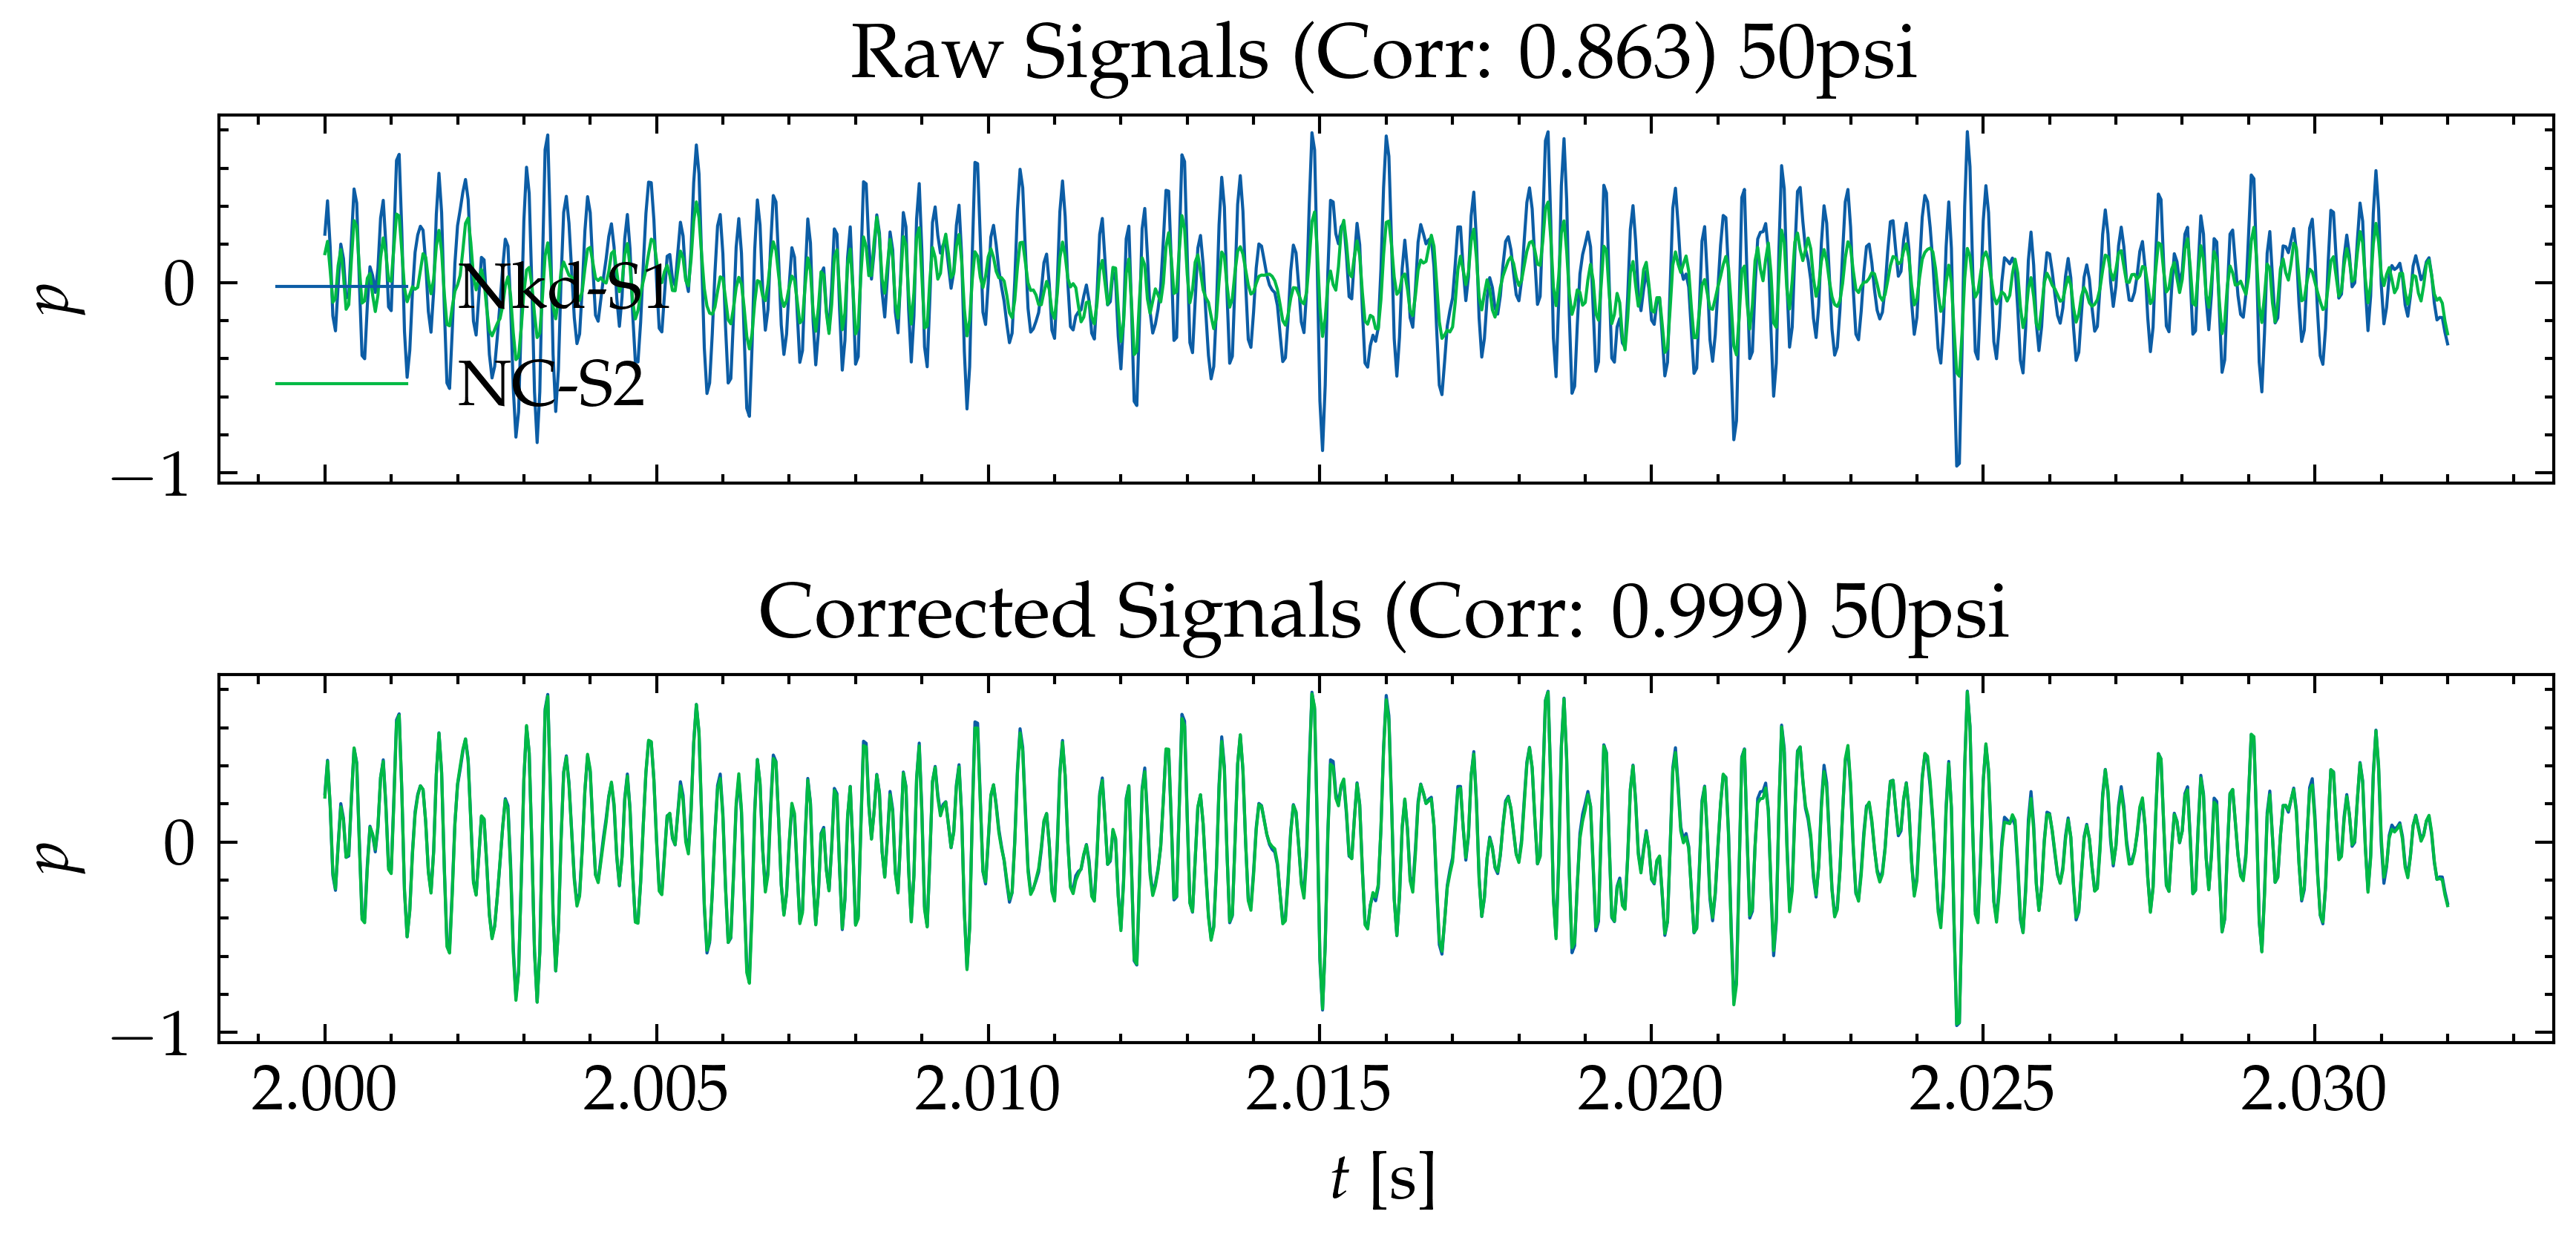
\includegraphics[width=\linewidth]{NC-NKD/y_50psi.png}
            % 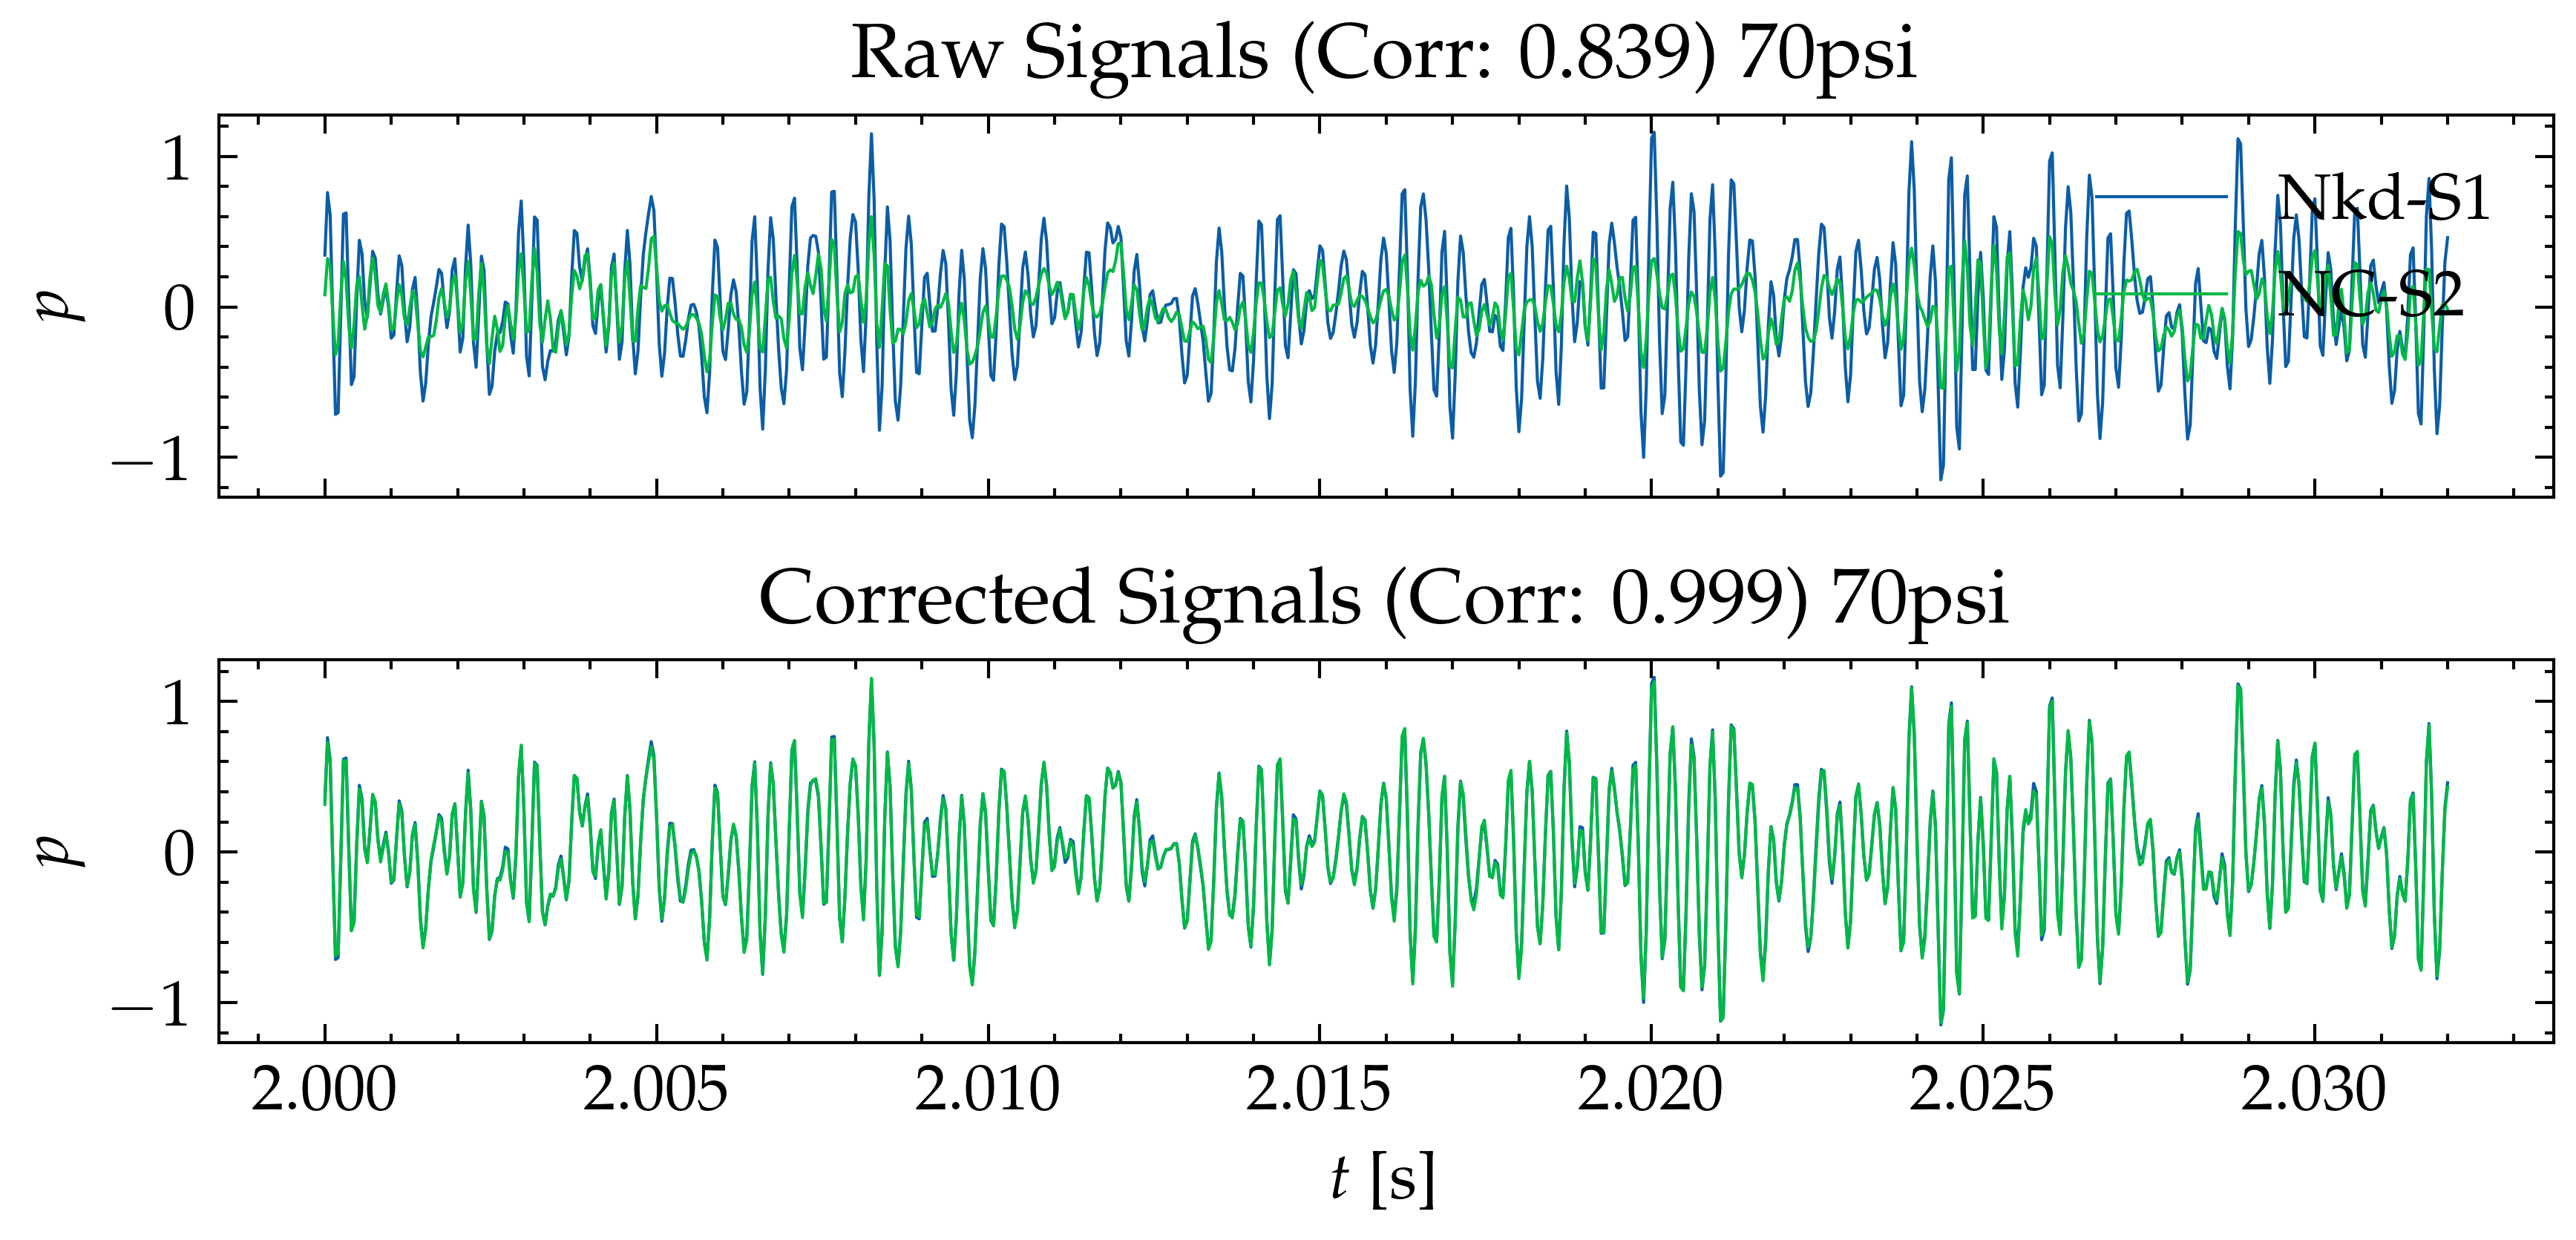
\includegraphics[width=\linewidth]{NC-NKD/y_70psi.png}
            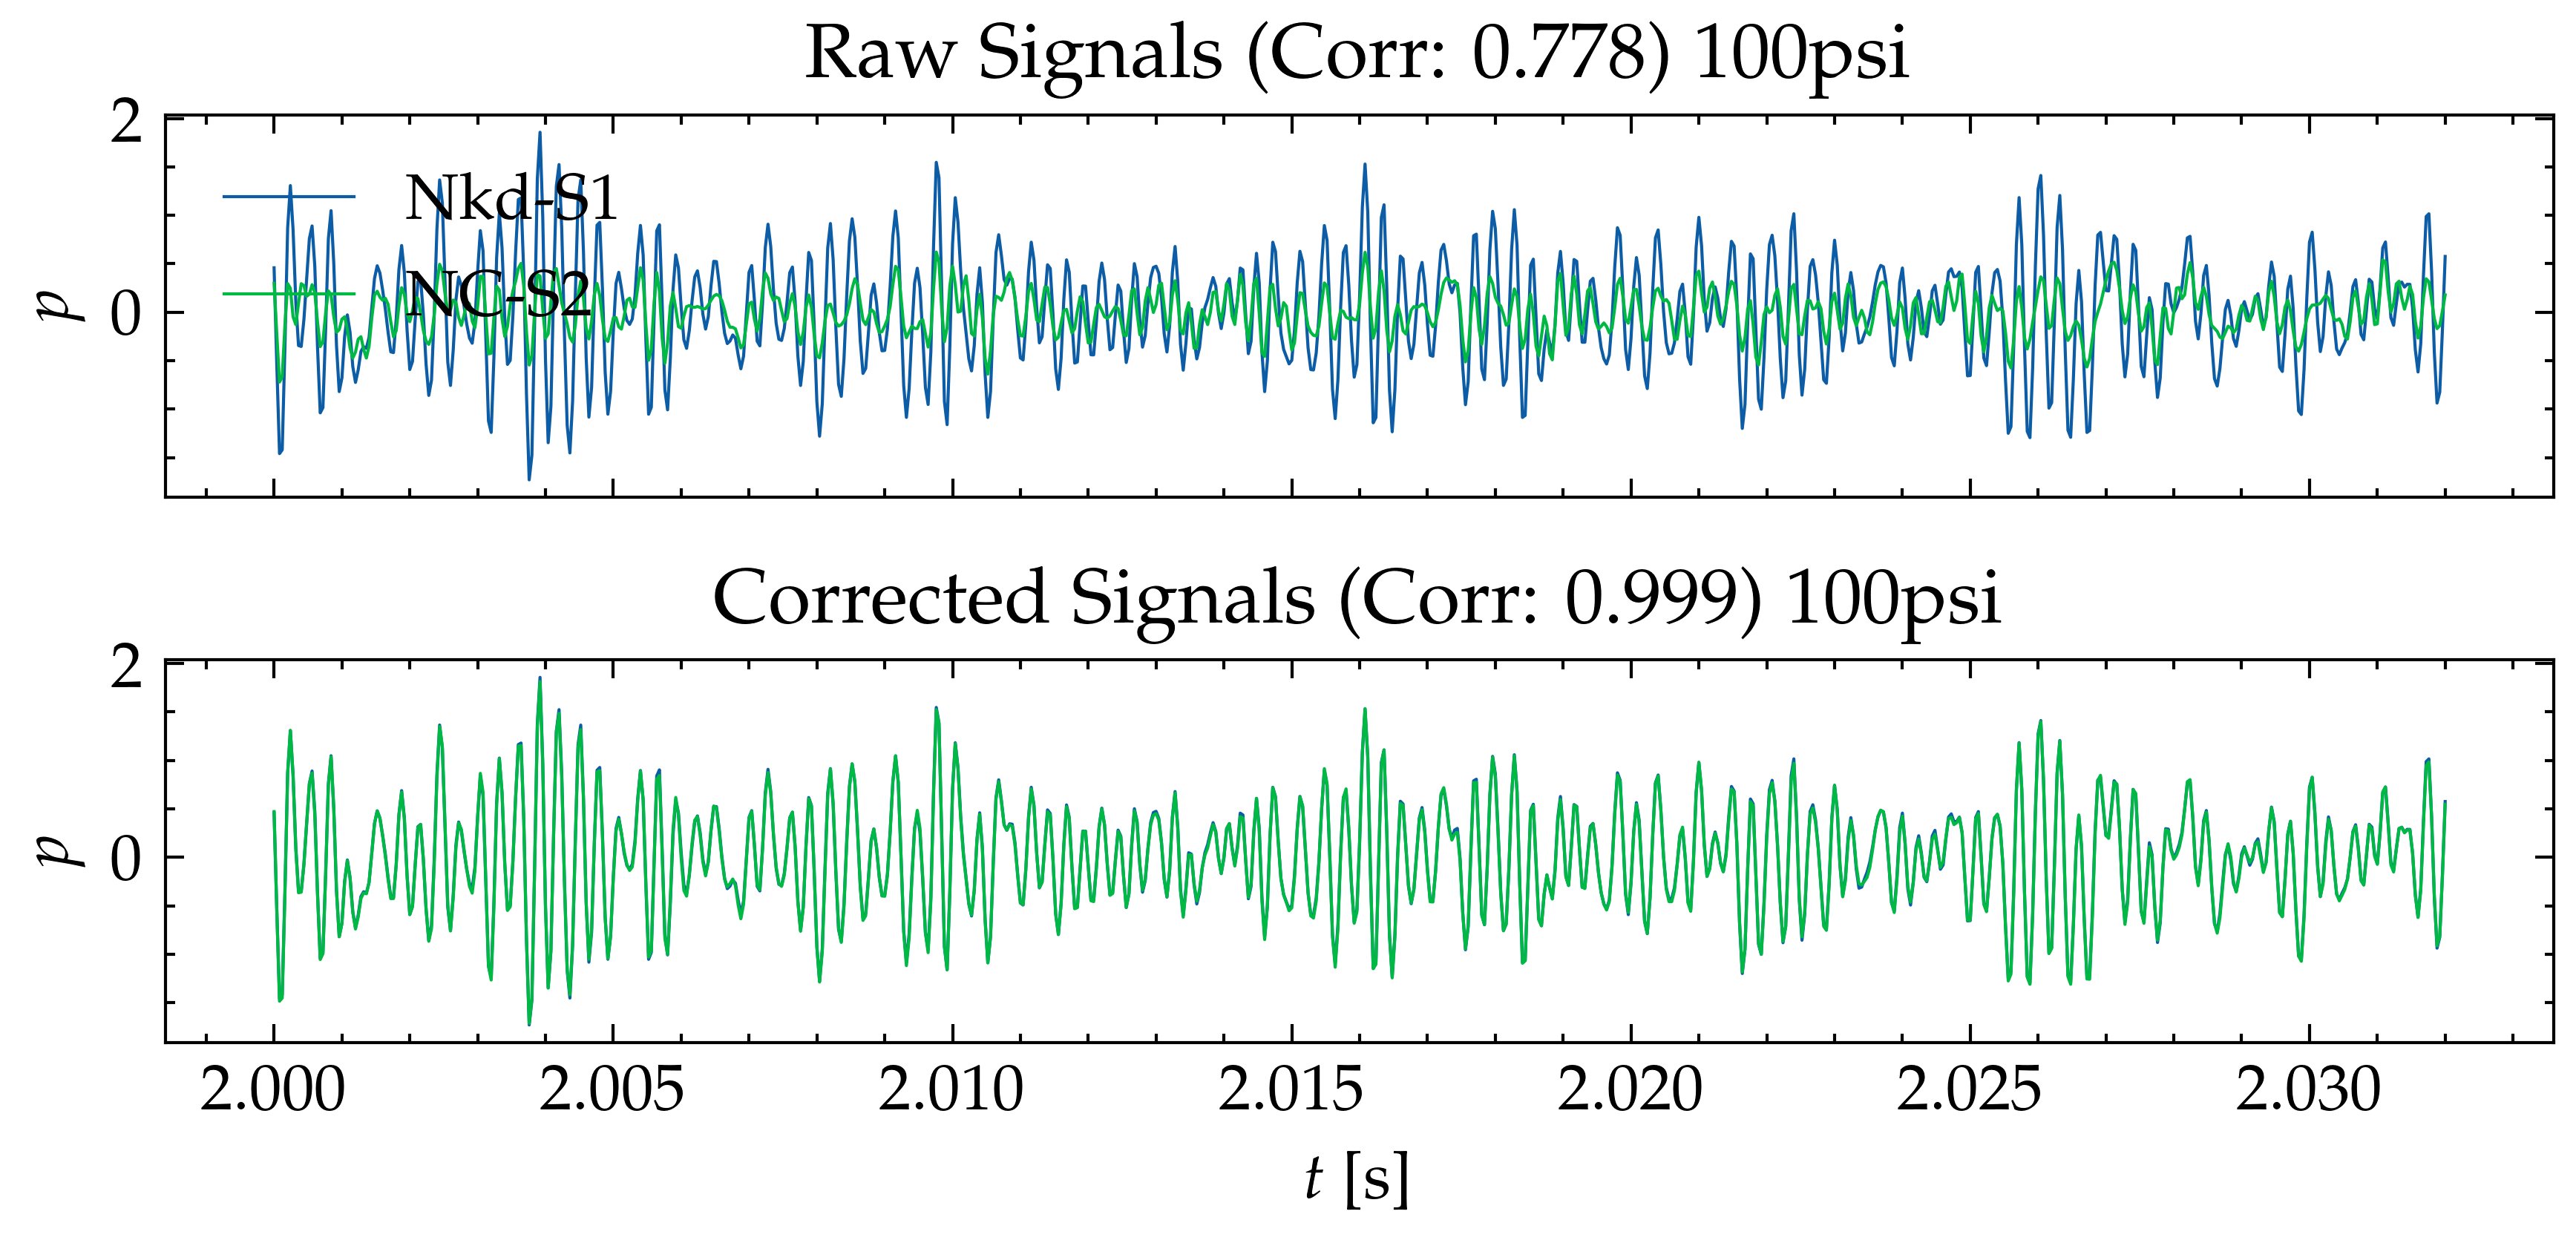
\includegraphics[width=\linewidth]{NC-NKD/y_100psi.png}
        \column{0.3\textwidth}
        \centering
            Corrected PH trace
            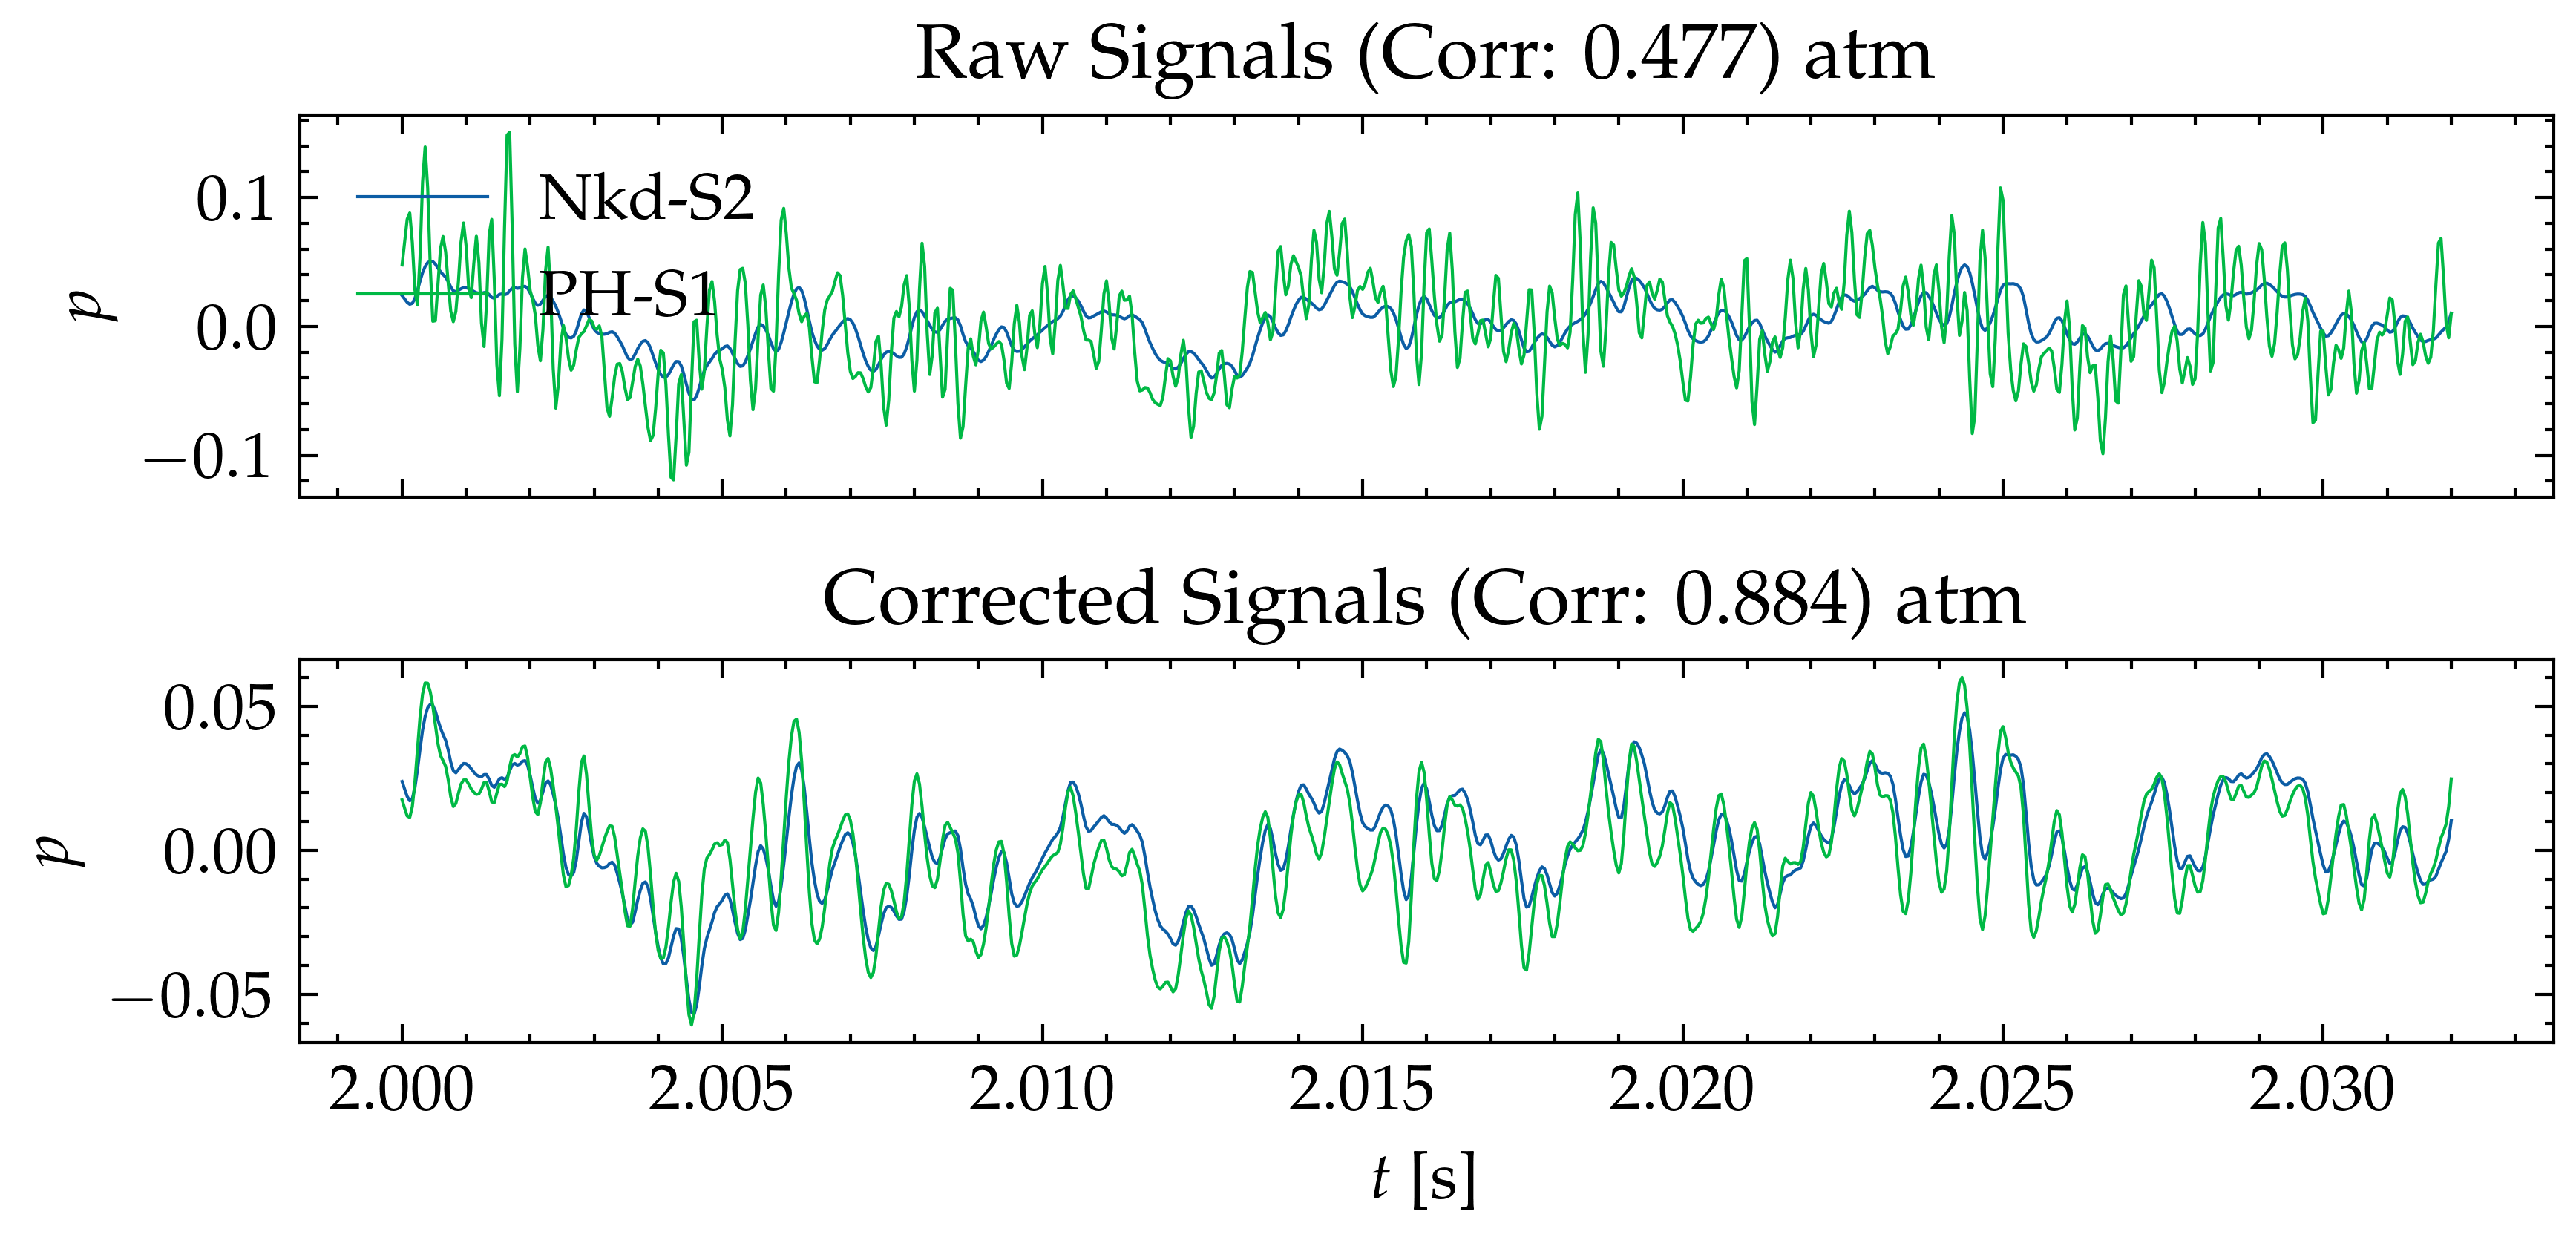
\includegraphics[width=\linewidth]{PH-NKD/y_atm.png}
            % 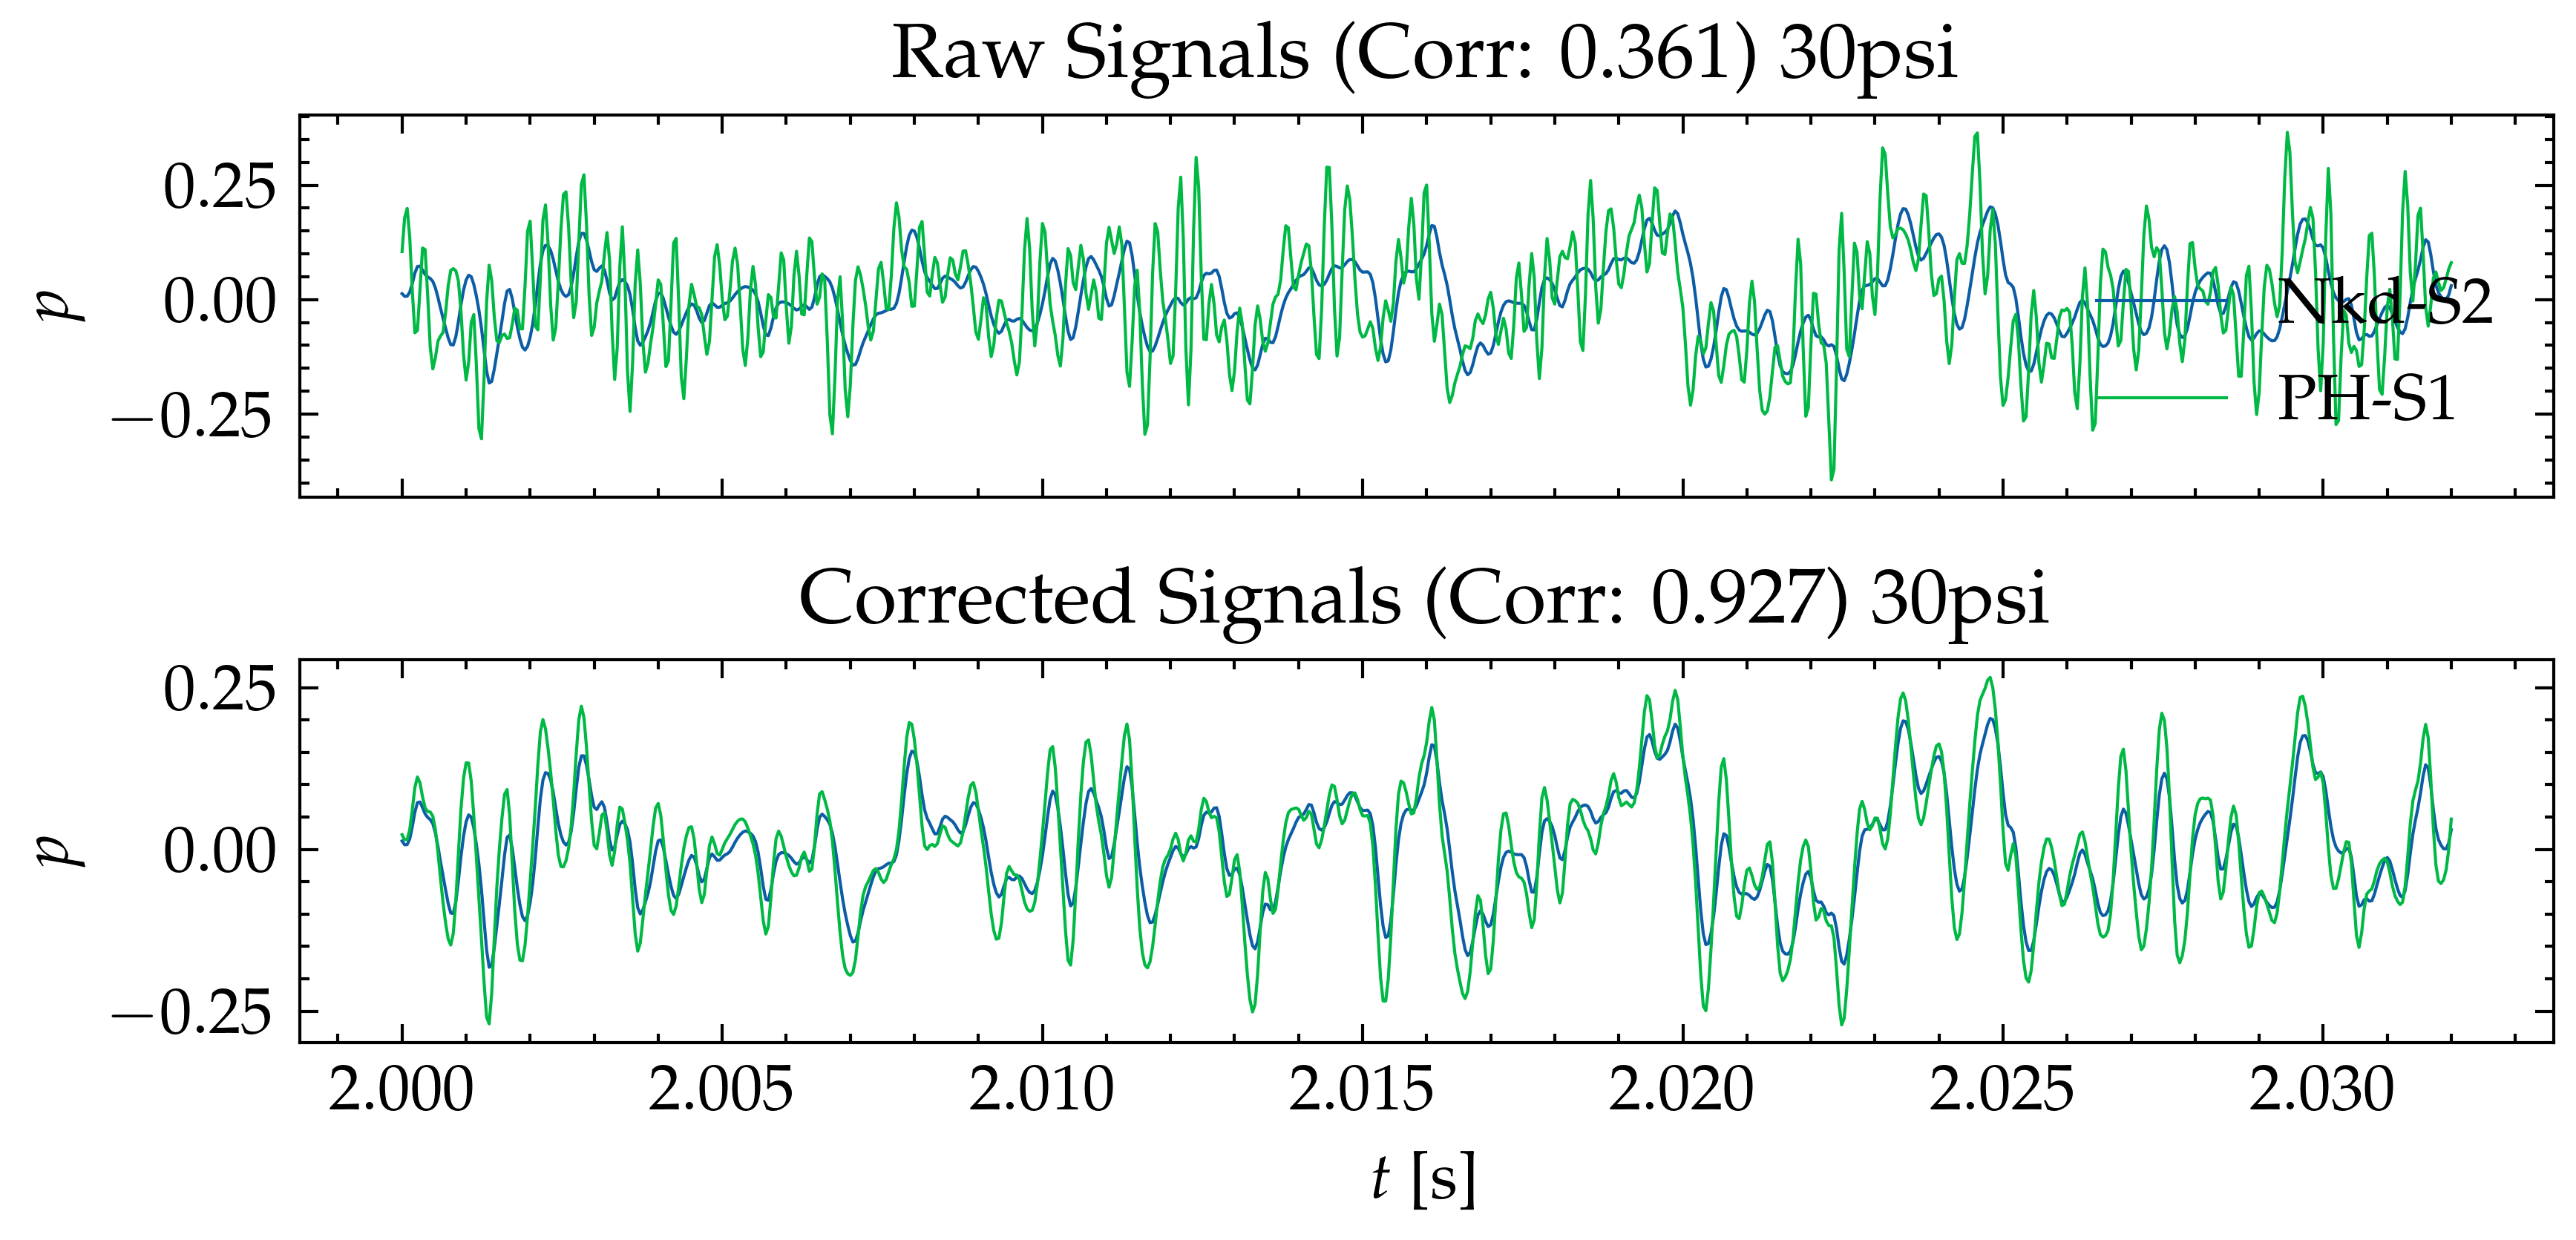
\includegraphics[width=\linewidth]{PH-NKD/y_30psi.png}
            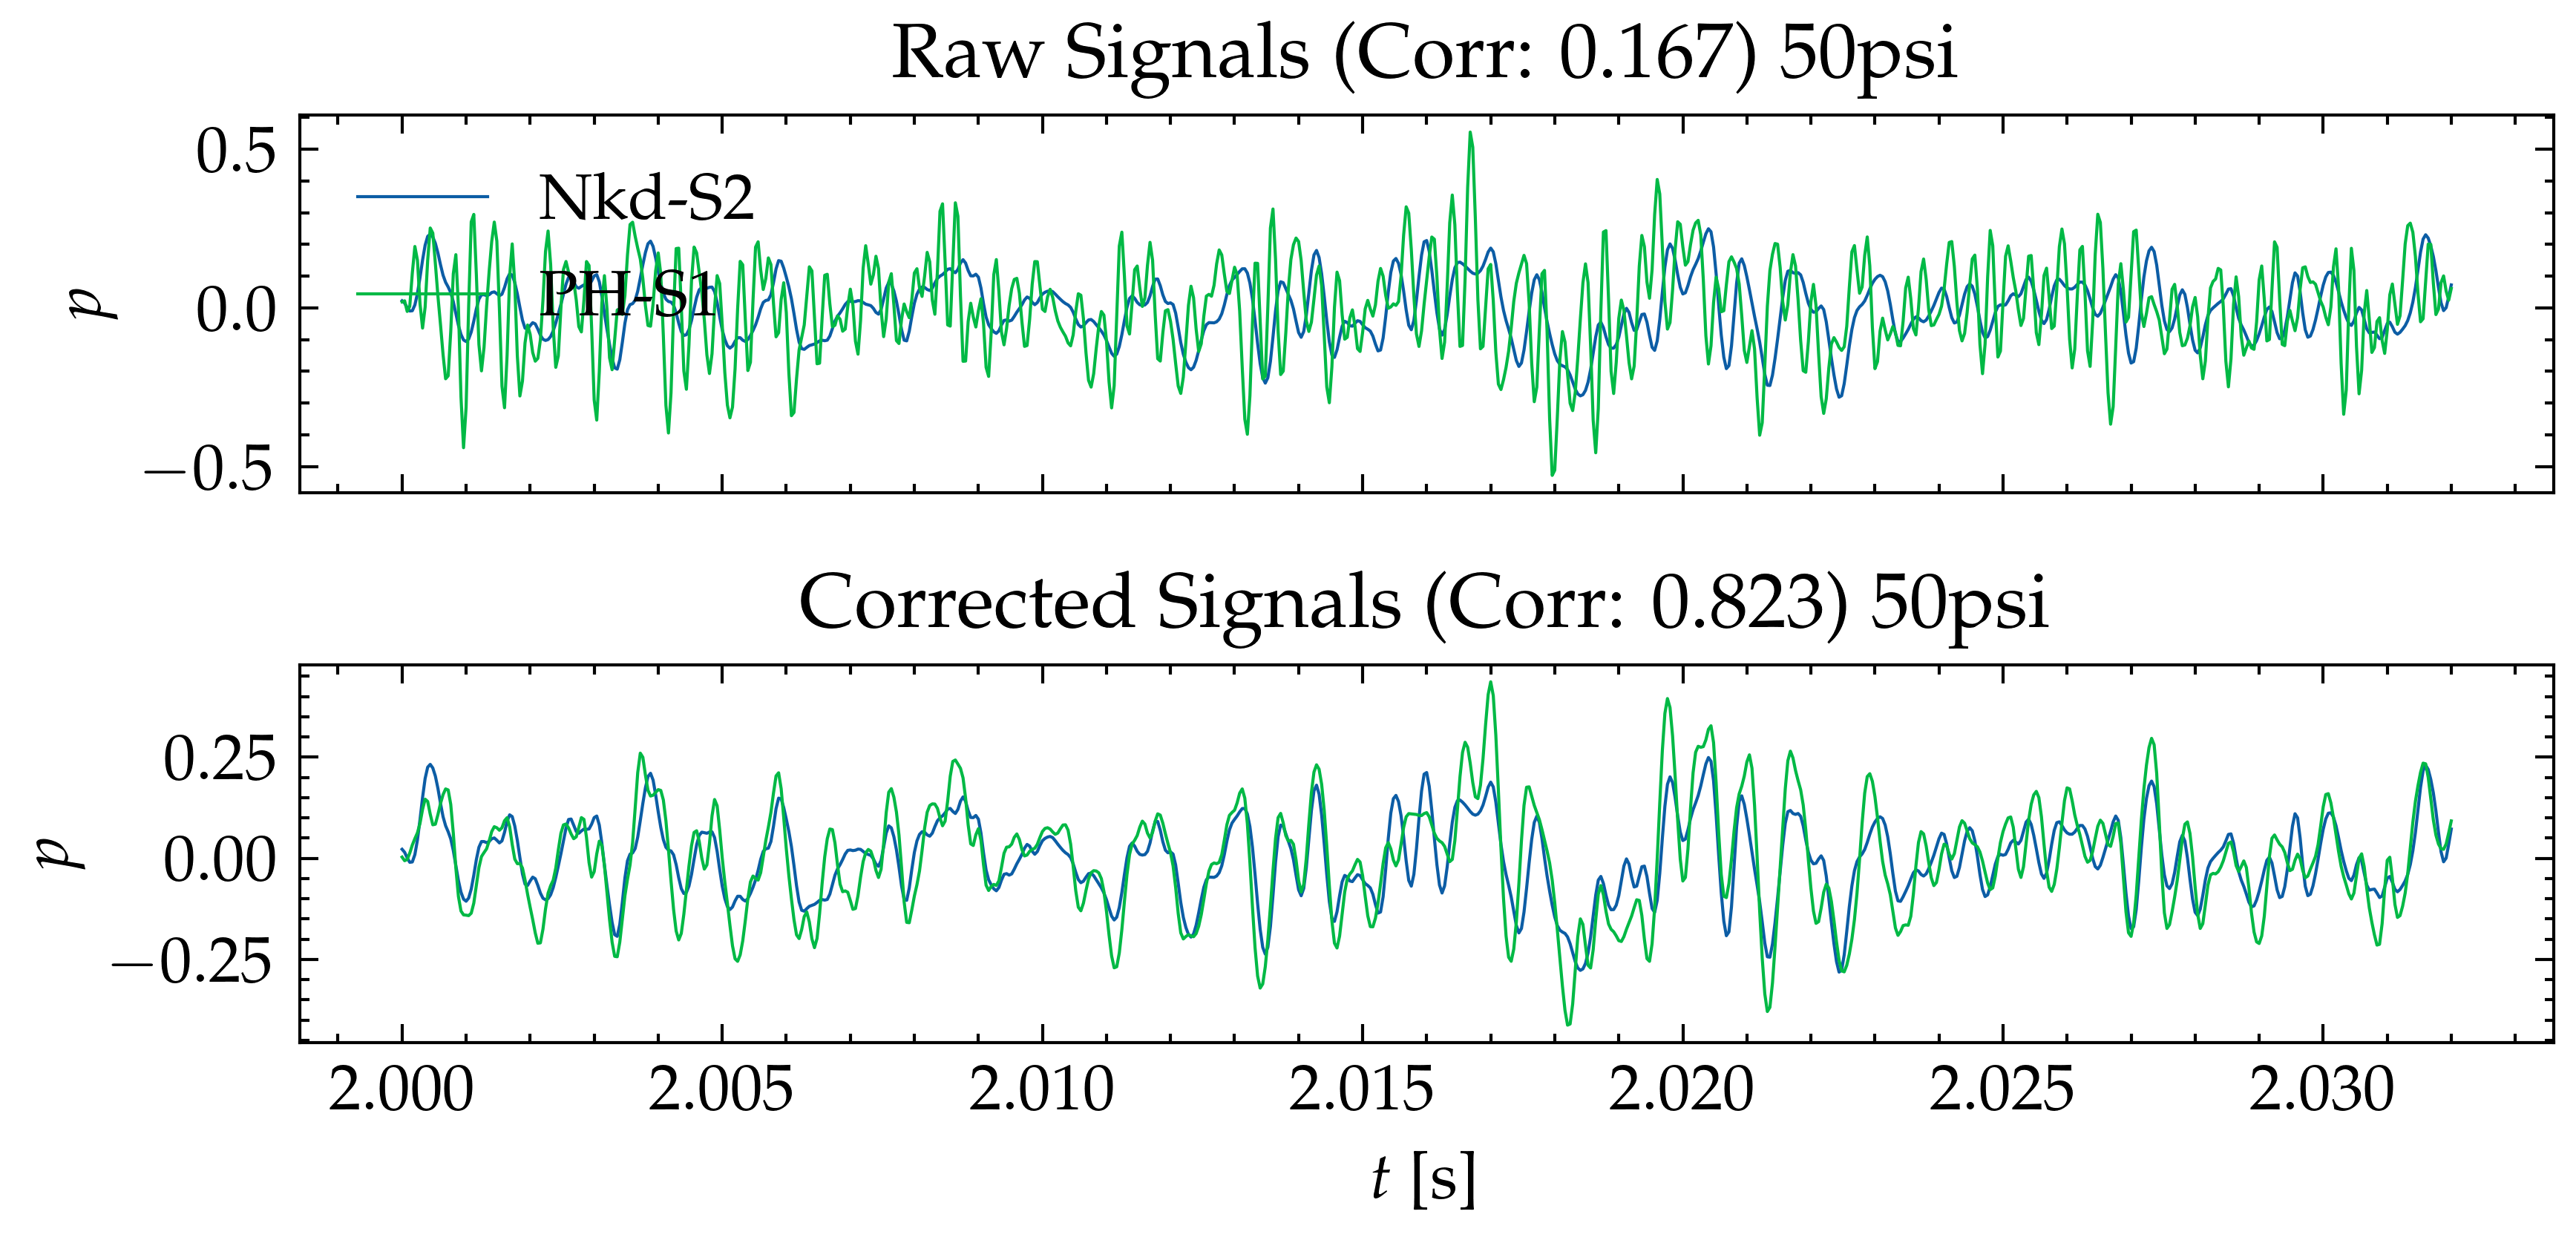
\includegraphics[width=\linewidth]{PH-NKD/y_50psi.png}
            % 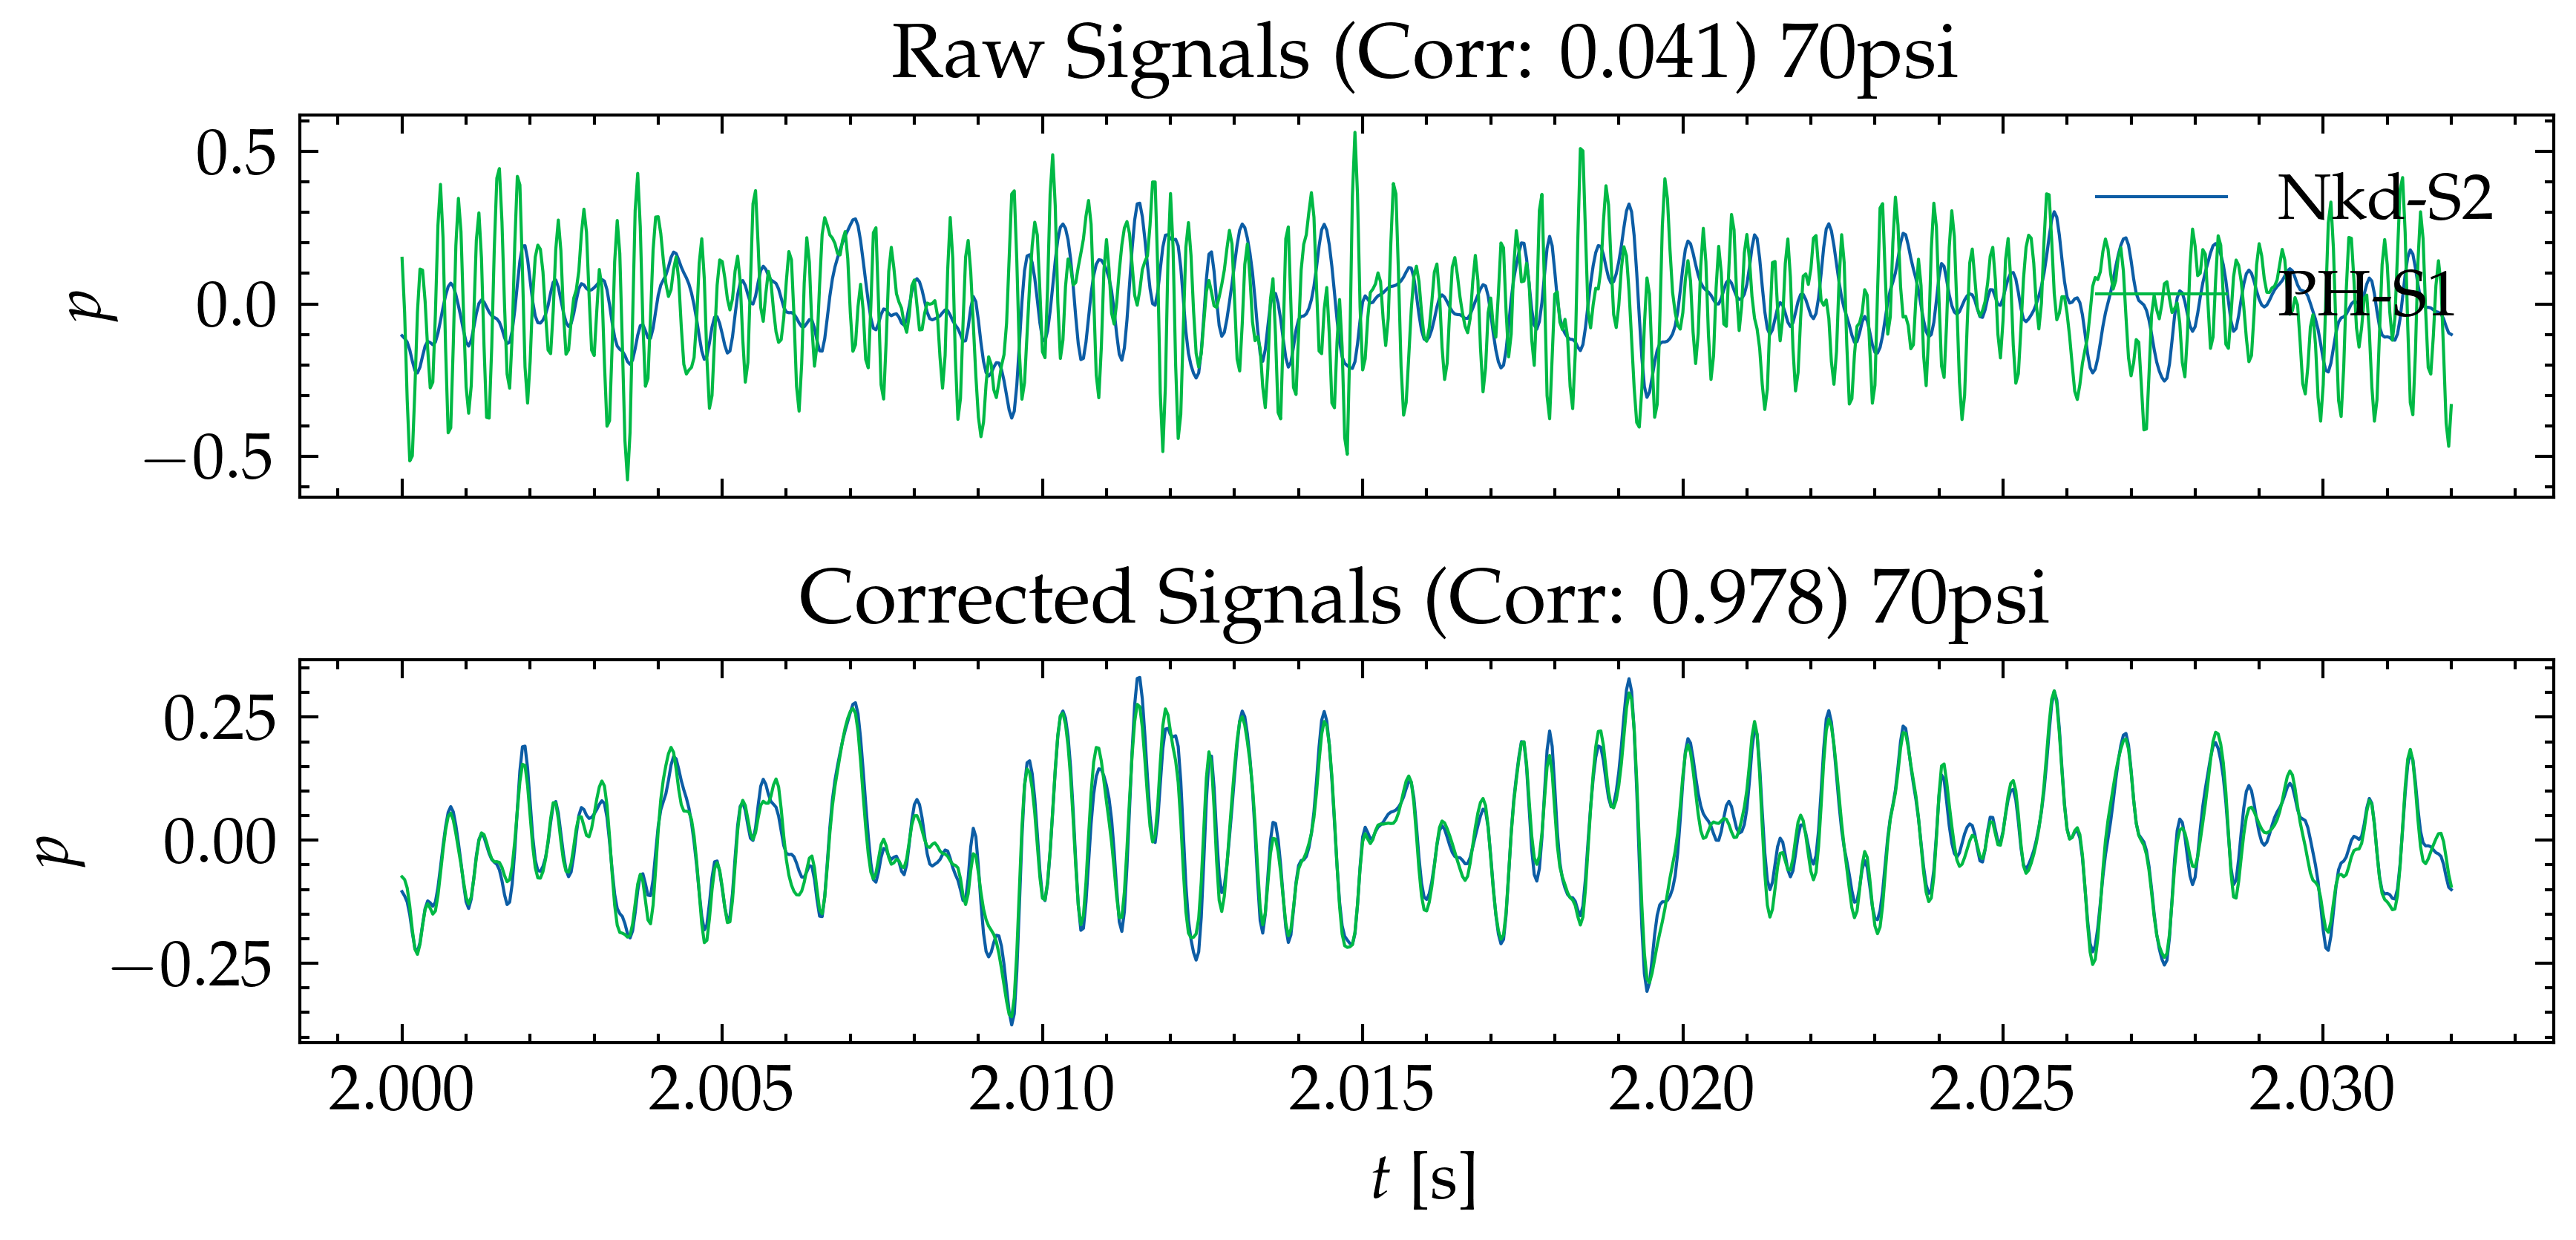
\includegraphics[width=\linewidth]{PH-NKD/y_70psi.png}
            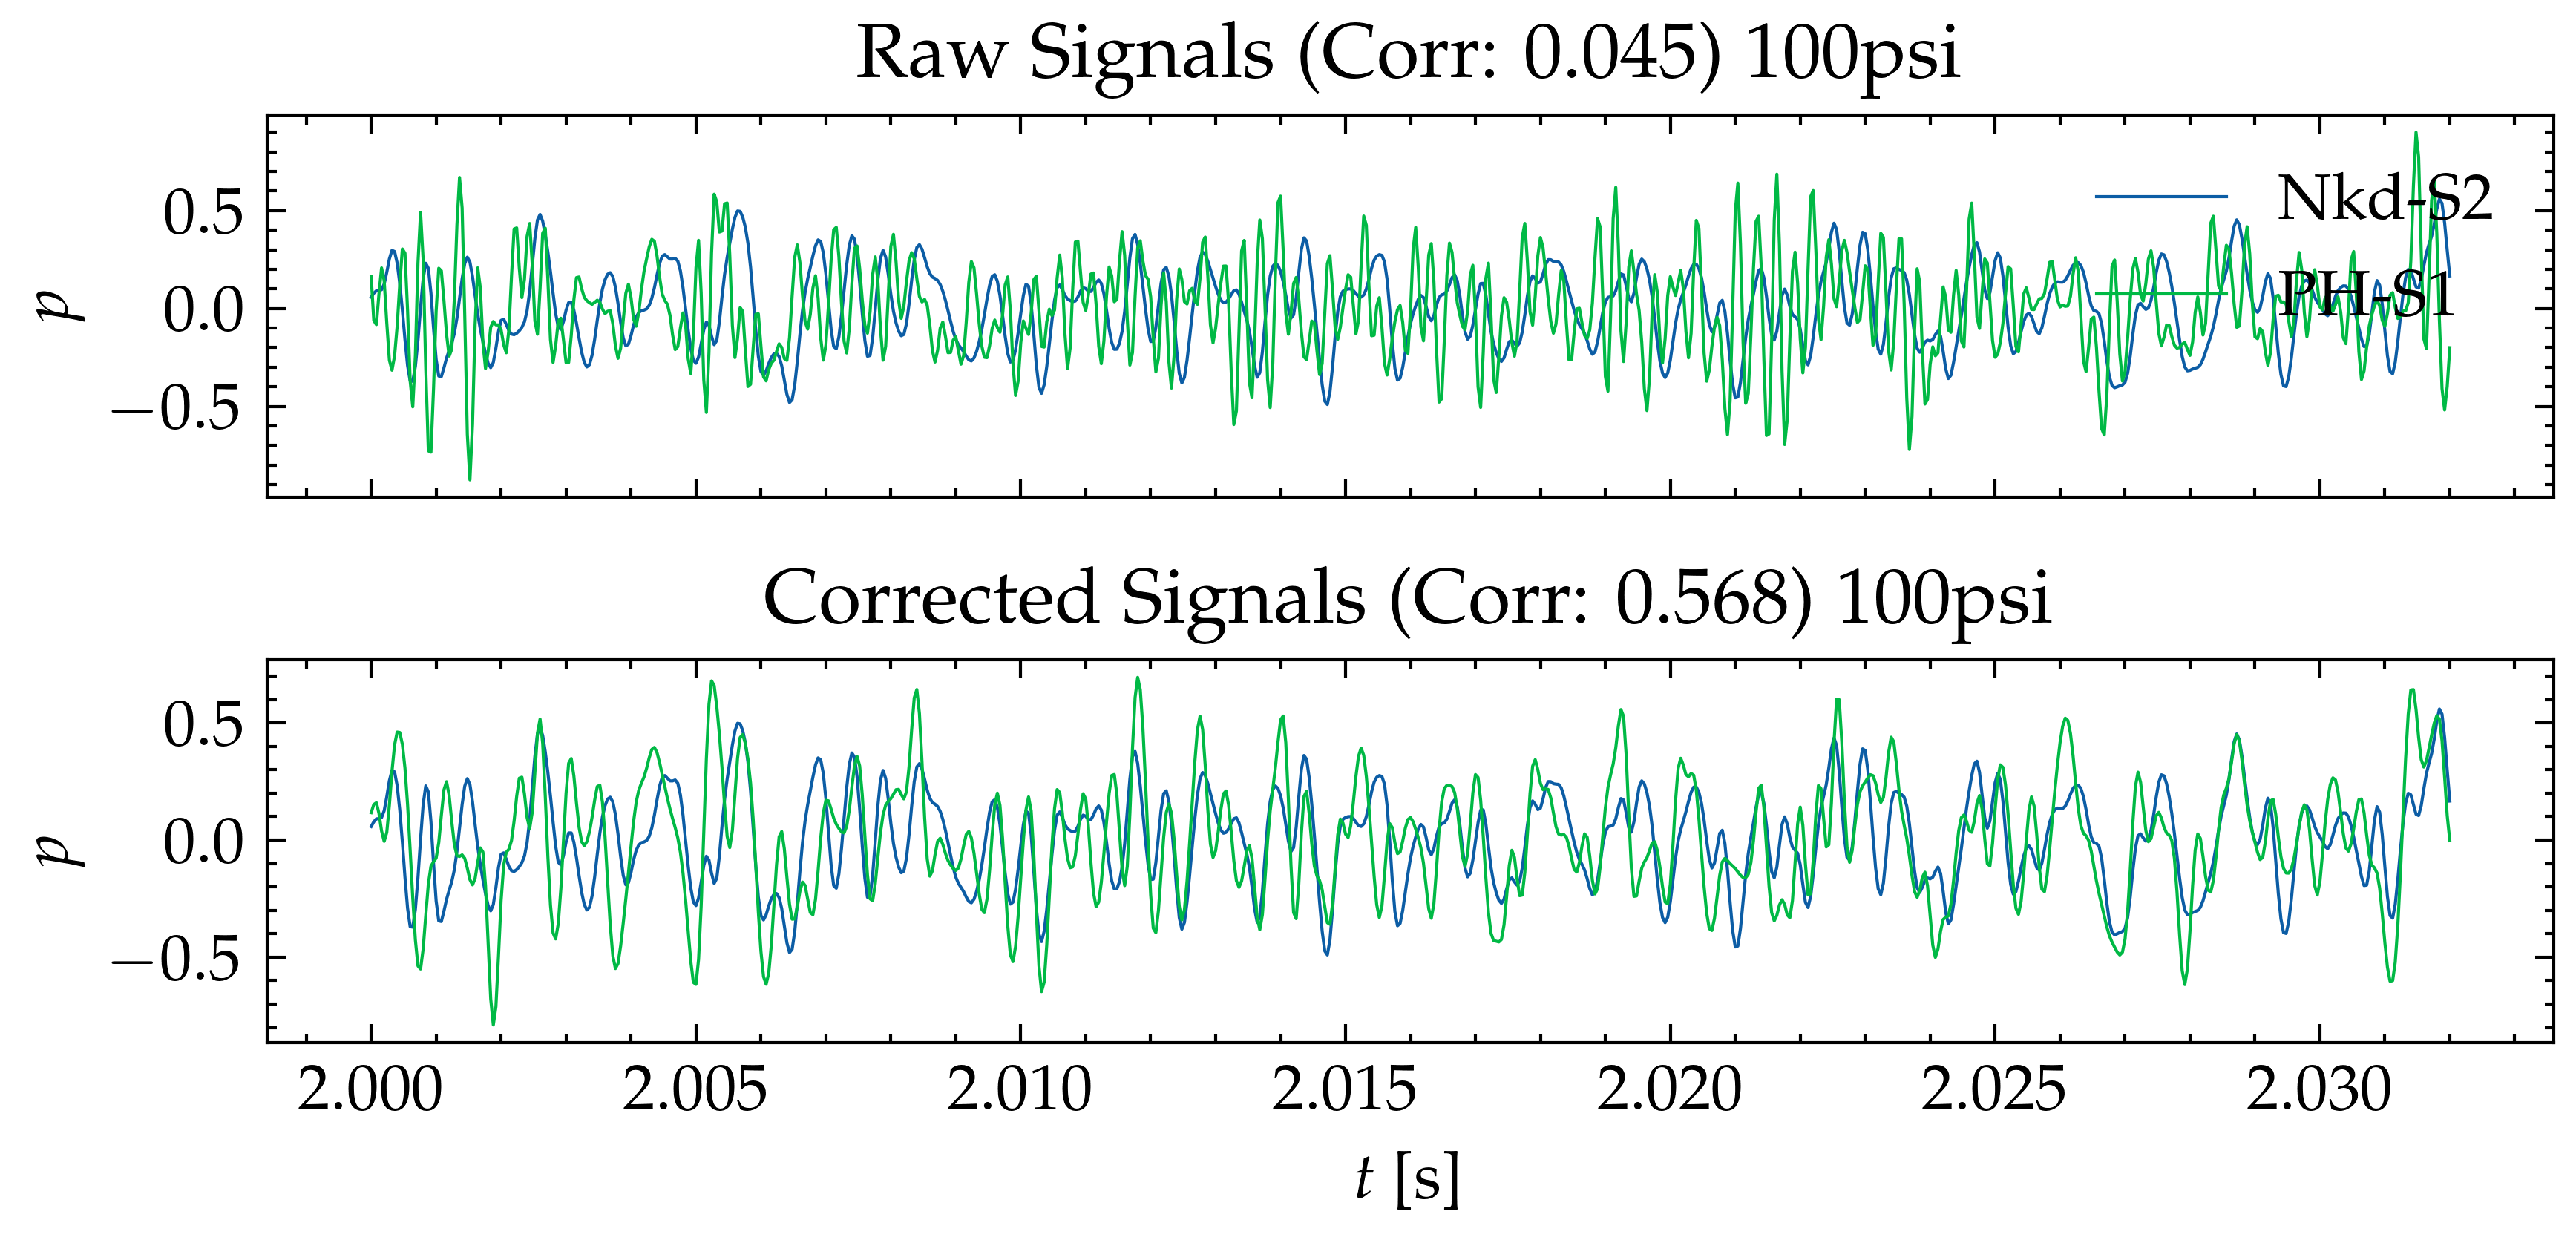
\includegraphics[width=\linewidth]{PH-NKD/y_100psi.png}
    \end{columns}
\end{frame}

\begin{frame}
    \frametitle{Raw vs corrected}
    \centering
    Corrected NC trace
    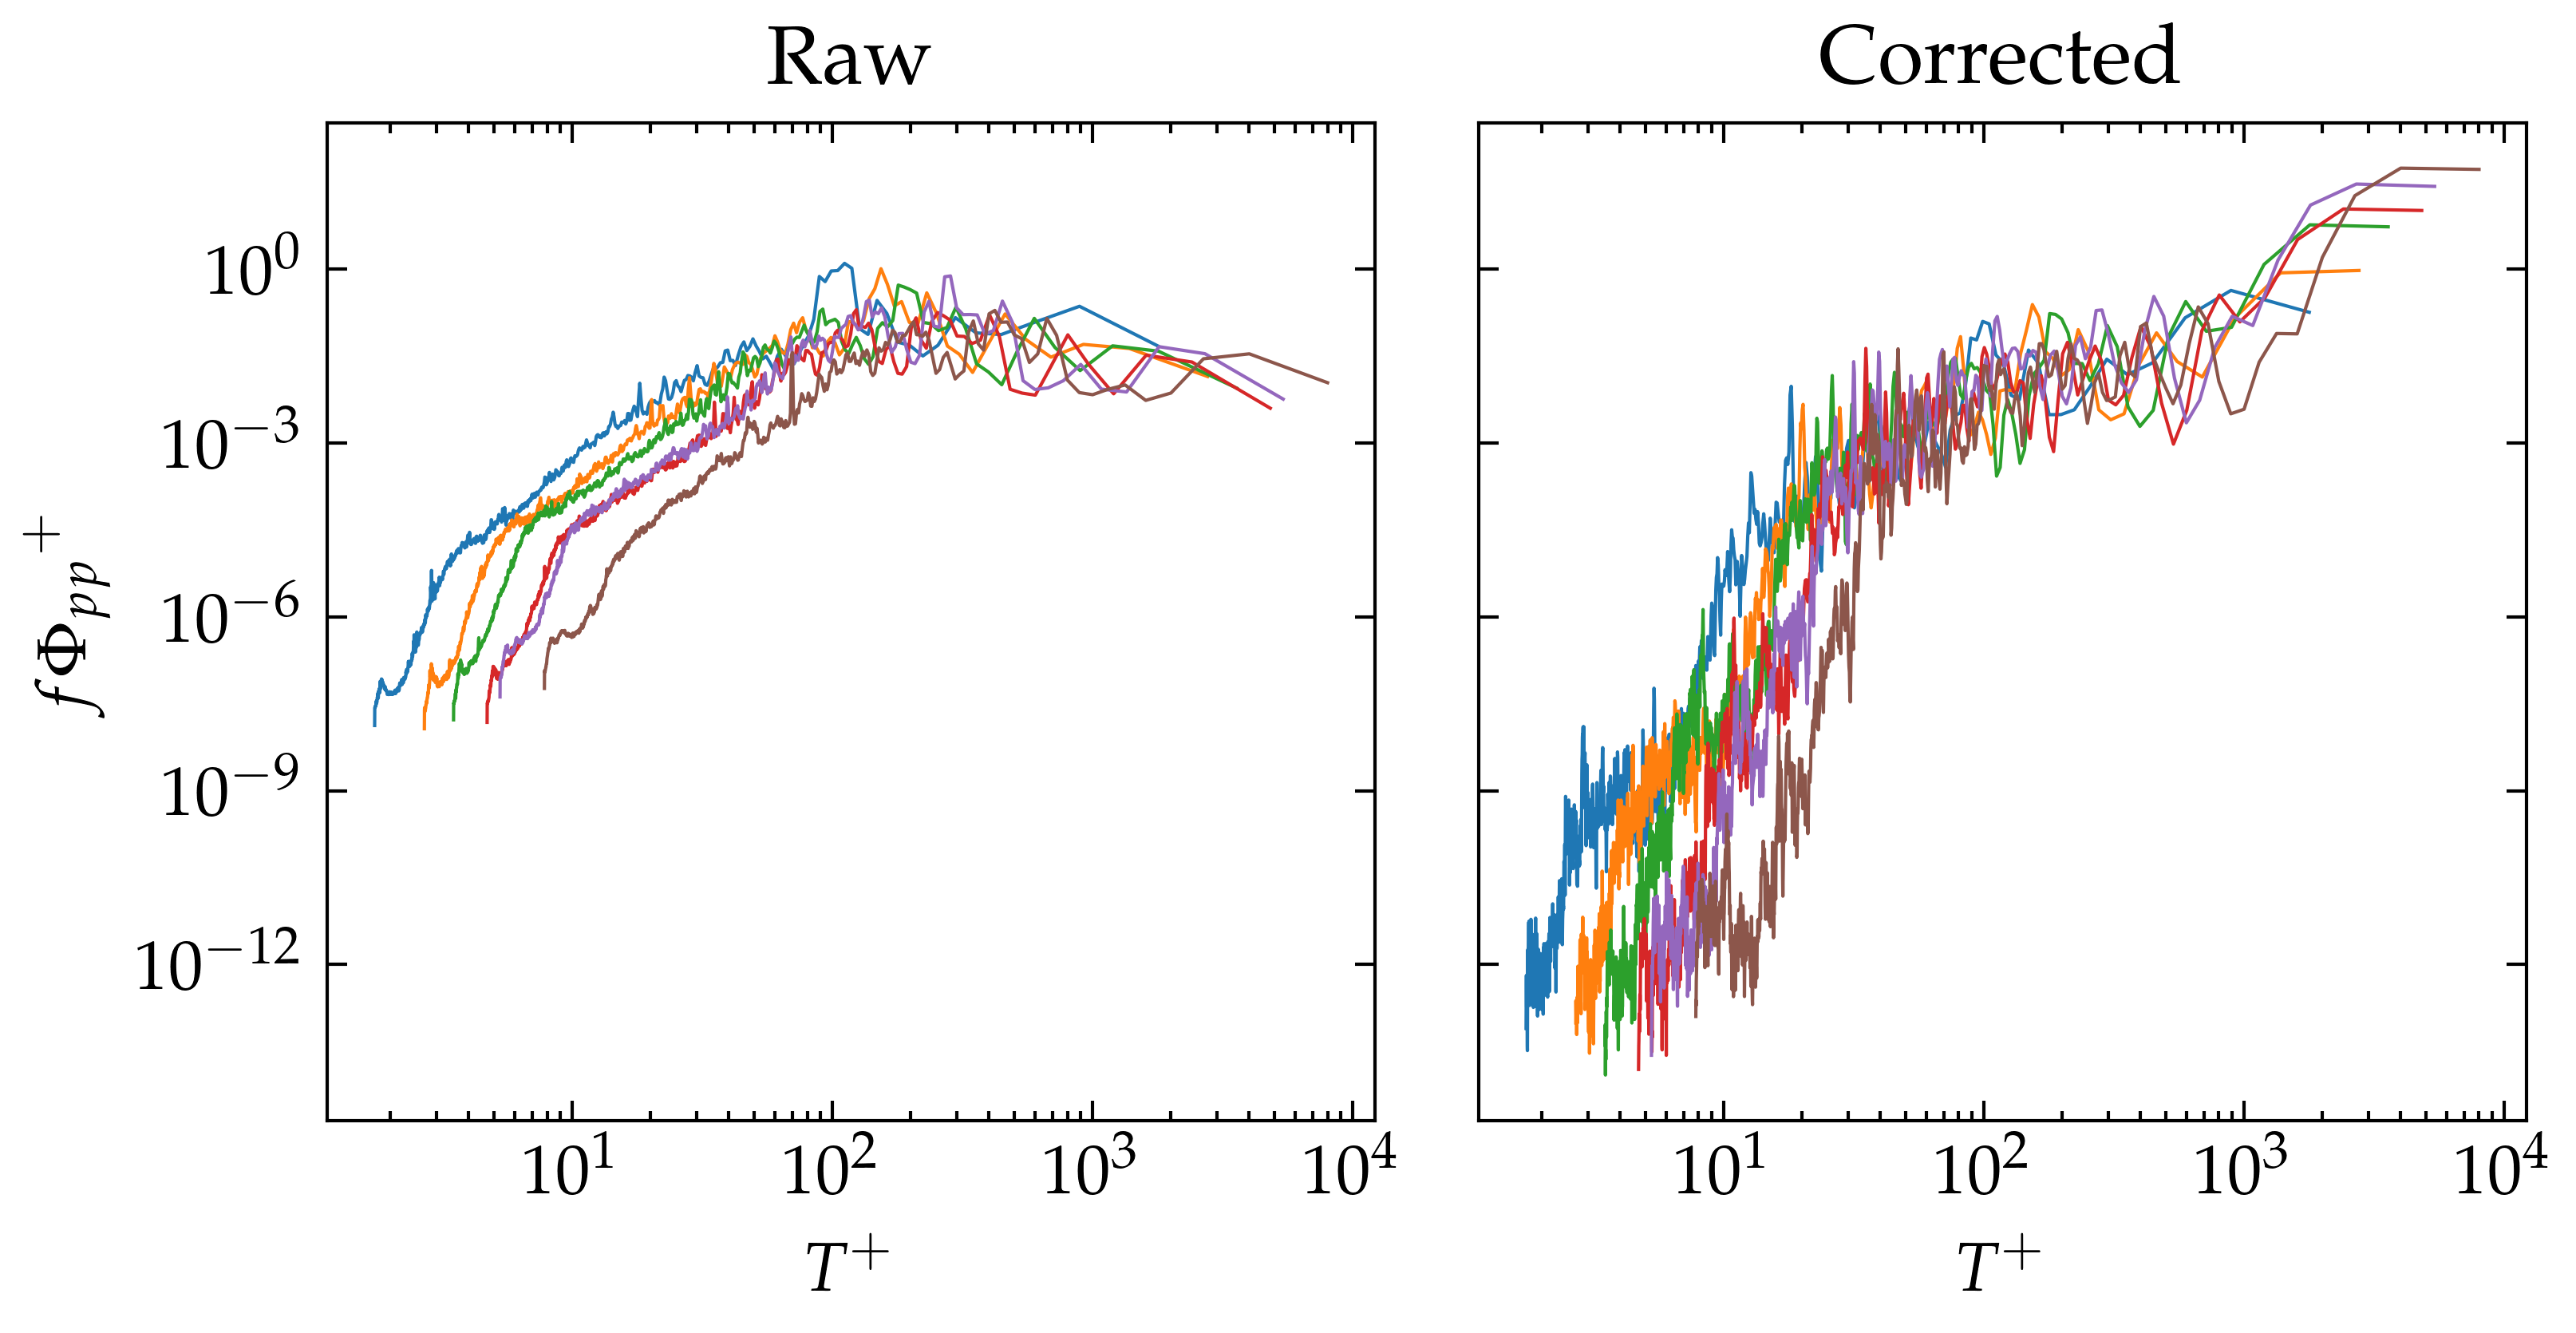
\includegraphics[width=\linewidth]{real/spectra/Pyy_log.png}
            
\end{frame}

\begin{frame}
  \frametitle{Calibration algos}
\begin{columns}[c]
\column{0.48\textwidth}
    \begin{algorithm}[H] % <-- H prevents floating inside columns
        \footnotesize
        \caption{$H$ Transfer-Function Estimation}\label{alg:H}
        \begin{algorithmic}[1]
            \Require $x[n]$ (ref), $y[n]$ (treated), $f_s$, Welch $(N_{\mathrm{seg}},N_{\mathrm{ov}},w)$
            \Ensure $f[k]$, $H[k]$, $\gamma^2[k]$
            \State Compute $S_{xx}[k],S_{yy}[k]$ (Welch)
            \State Compute $S_{xy}[k]$ (same settings)
            \State $H[k]\gets S_{xy}[k]/S_{xx}[k]$
            \State $\gamma^2[k]\gets |S_{xy}[k]|^2/(S_{xx}[k]S_{yy}[k])$
            \State \Return $(f[k],H[k],\gamma^2[k])$
        \end{algorithmic}
    \end{algorithm}
    \column{0.48\textwidth}
        \begin{algorithm}[H]
            \footnotesize
            \caption{Coherence-weighted Wiener inverse}\label{alg:inv}
            \begin{algorithmic}[1]
                \Require $y_r$, $f_s$, grid $f$, $H(f)$, $\gamma^2(f)$
                \Ensure $y$
                \State $y_r \leftarrow y_r - \mathrm{mean}(y_r)$
                \State $\hat{y}_r\gets\mathcal{F}(y_r,N_{\mathrm{fft}})$
                \State $m\gets|H|$, $\ \phi\gets\mathrm{unwrap}(\angle H)$
                \State Interp $m,\phi,\gamma^2$ to FFT grid $\Rightarrow m_i,\phi_i,\gamma_i^2$
                \State $H_i\gets m_i\,e^{j\phi_i}$;\ \ $\varepsilon\gets$ machine epsilon
                \State $H_{\!inv}\gets \gamma_i^2\,H_i^{\!*}/\max(m_i^2,\varepsilon)$
                \State $H_{\!inv}[0]\gets 0$ \quad(\& Nyquist if present)
                \State $y\gets \Re\!\left\{\mathcal{F}^{-1}\!\big(\hat{y}_r\cdot H_{\!inv}\big)[0{:}N]\right\}$
                \State \Return $y$
            \end{algorithmic}
        \end{algorithm}

  \end{columns}
\end{frame}


% \begin{frame}[noframenumbering,allowframebreaks]
%     \frametitle{References}
%     \bibliographystyle{jfm}
%     \bibliography{refs}
% \end{frame}

\end{document}
